\documentclass[runningheads]{llncs}
\usepackage[T1]{fontenc}
\usepackage{amsmath,amssymb,amsfonts}
\allowdisplaybreaks[1]
\usepackage{mathtools}
\usepackage{enumitem}
\setlist[enumerate]{topsep=0pt,itemsep=1ex,partopsep=0ex,parsep=0.5ex}
\usepackage{thmtools, thm-restate}
\usepackage{caption}

\usepackage{algorithm}
\usepackage{algpseudocode}
\usepackage{needspace}
\usepackage[section]{placeins}

\usepackage{graphicx}
\usepackage{tikz}
\usetikzlibrary{arrows,calc,positioning}
\usepackage{booktabs, multirow, makecell, array}

\DeclarePairedDelimiter\ceil{\lceil}{\rceil}
\DeclarePairedDelimiter\floor{\lfloor}{\rfloor}

\setcounter{secnumdepth}{3}

\usepackage{etoolbox}
\usepackage{xcolor}
\patchcmd{\paragraph}{\itshape}{\bfseries}{}{}

\usepackage[hidelinks, colorlinks=true, linkcolor=blue, citecolor=blue, urlcolor=blue, hyperfootnotes=true, bookmarksdepth=2]{hyperref}
\AddToHook{cmd/appendix/before}{%
  \gdef\theHsection{app.\Alph{section}}%
  \gdef\theHsubsection{app.\Alph{section}.\arabic{subsection}}%
  \gdef\theHsubsubsection{app.\Alph{section}.\arabic{subsection}.\arabic{subsubsection}}%
}

\usepackage{booktabs}
\usepackage{longtable}
\usepackage{array}
\usepackage{listings}
\lstdefinestyle{llncs}{
  basicstyle=\ttfamily\footnotesize,
  columns=fullflexible,
  numbers=left, numberstyle=\tiny, numbersep=6pt,
  frame=single,
  breaklines=true, breakatwhitespace=true,
  tabsize=2,
  showstringspaces=false,
  captionpos=b,
  mathescape=false, texcl=false
}
\lstset{style=llncs}


\newcommand{\FlatEnv}[1]{%
  \AtBeginEnvironment{#1}{\par\noindent\setlength{\parindent}{0pt}}%
}
\FlatEnv{theorem}
\FlatEnv{lemma}
\FlatEnv{proposition}
\FlatEnv{corollary}
\FlatEnv{definition}
\FlatEnv{claim}
\FlatEnv{proof}
% \FlatEnv{Heuristic}
\AtBeginEnvironment{proof}{\par\noindent\setlength{\parindent}{0pt}}
\AtEndEnvironment{proof}{\hfill\qed\par}
\providecommand{\qed}{\hfill\ensuremath{\square}}

\floatname{algorithm}{Algorithm}
\renewcommand{\thealgorithm}{\arabic{algorithm}}

\usepackage{chngcntr}
\counterwithout{algorithm}{section}
\usepackage[nocompress]{cite}

\spnewtheorem{heuristic}{Heuristic}{\bfseries}{\itshape}

\usepackage{listings}
\usepackage{xcolor}
\definecolor{codegreen}{rgb}{0,0.6,0}
\definecolor{codegray}{rgb}{0.5,0.5,0.5}
\definecolor{codepurple}{rgb}{0.58,0,0.82}
\definecolor{backcolour}{rgb}{0.98,0.98,0.98}
\lstdefinelanguage{Sage}[]{Python}{
  morekeywords={True, False, sage, ZZ, QQ, GF, EllipticCurve, isogeny, is_supersingular, order, random_element},
  sensitive=true
}
\lstdefinestyle{sagestyle}{
    backgroundcolor=\color{backcolour},   
    commentstyle=\color{codegreen}\itshape,
    keywordstyle=\color{blue}\bfseries,
    numberstyle=\tiny\color{codegray},
    stringstyle=\color{codepurple},
    basicstyle=\ttfamily\footnotesize,
    breakatwhitespace=false,         
    breaklines=true,             
    captionpos=b,                     
    keepspaces=true,                 
    numbers=left,           
    numbersep=5pt,                  
    showspaces=false,                
    showstringspaces=false,
    showtabs=false,                  
    tabsize=4,
    frame=lines             
}

\usepackage[most]{tcolorbox}
\newtcolorbox{algobox}{
    enhanced,
    breakable,
    colback=white,
    colframe=black,
    boxrule=0.8pt,
    arc=2pt,
    left=6pt,
    right=6pt,
    top=6pt,
    bottom=6pt
}
% \newcommand{\algoboxstart}{%
%   \par\medskip
%   \noindent\hrule height 0.4pt
%   \vspace{0.35em}
%   \noindent\ignorespaces
% }

% \newcommand{\algoboxend}{%
%   \par\vspace{0.25em}
%   \noindent\hrule height 0.4pt
%   \medskip
% }

\newcommand{\redstrike}[1]{%
  \tikz[baseline=(txt.base)]{
    \node[inner sep=0pt, outer sep=0pt, anchor=base] (txt) {#1};
    \draw[red, line width=1pt]
      ($(txt.south west)+(0,0.9ex)$) -- ($(txt.south east)+(0,0.9ex)$);
  }%
}
\newcommand{\replacebelow}[2]{%
  \begingroup
  \setbox0=\hbox{#1}%
  \leavevmode
  \makebox[\wd0][l]{%
    \rlap{\raisebox{-1.05em}[0pt][1.15em]{\textcolor{blue}{#2}}}%
    #1%
  }%
  \endgroup
}


% ==================================================
% Macros
% ==================================================

\newcommand{\Q}{\mathbb{Q}}
\newcommand{\Z}{\mathbb{Z}}
\newcommand{\N}{\mathbb{N}}
\newcommand{\R}{\mathbb{R}}
\newcommand{\C}{\mathbb{C}}
\newcommand{\F}{\mathbb{F}}
\newcommand{\Fp}{\mathbb{F}_p}
\newcommand{\Fpp}{\mathbb{F}_{p^2}}
\newcommand{\lcm}{\mathrm{lcm}}

\newcommand{\End}{\mathrm{End}}
\newcommand{\Hom}{\mathrm{Hom}}

\newcommand{\calO}{\mathcal{O}}
\newcommand{\Bp}{B_{p,\infty}}
\newcommand{\trd}{\mathrm{trd}}
\newcommand{\nrd}{\mathrm{nrd}}

\newcommand{\rad}{\operatorname{rad}}
\newcommand{\radinf}{\operatorname{rad}_{\infty}}
\newcommand{\midpoint}{\operatorname{mid}}
\newcommand{\adj}{\operatorname{adj}}

\newcommand{\pp}{\mathsf{pp}}
\newcommand{\pk}{\mathsf{pk}}
\newcommand{\sk}{\mathsf{sk}}

\newcommand{\KeyGen}{\mathsf{KeyGen}}
\newcommand{\Sign}{\mathsf{Sign}}
\newcommand{\Verify}{\mathsf{Verify}}

\newcommand{\sample}{\xleftarrow{\$}}

\newcommand{\Dmix}{D_\text{mix}}
\newcommand{\Drsp}{D_\text{rsp}}
\newcommand{\qrsp}{q_\text{rsp}}
\newcommand{\ersp}{e_\text{rsp}}
\newcommand{\coeffbound}{\text{QUAT\_equiv\_bound\_coeff}}
\newcommand{\Isk}{I_\text{sk}}
\newcommand{\Icom}{I_\text{com}}
\newcommand{\Ichl}{I_\text{chl}}
\newcommand{\Icomrsp}{I_\text{com,rsp}}
\newcommand{\Iaux}{I_\text{aux}}

\title{Compact Quaternion Algorithms for SQIsign}
\author{Anonymous}
\institute{Anonymous}
\authorrunning{Anonymous}

\begin{document}

\maketitle

\begin{abstract}
SQIsign is an isogeny-based post-quantum signature scheme whose public keys and signatures are remarkably compact.
% Its practical efficiency, however, relies on arithmetic in quaternion algebras over the rational field.
% This quaternionic representation makes fixed-precision implementation difficult, since intermediate integer coefficients can grow much larger than the final cryptographic objects.
However, since SQIsign relies on arithmetic in quaternion algebras over the rational field, there was no fixed-precision integer arithmetic of SQIsign, hindering constant-time and implementation on memory-constrained devices.
Recent work by Kim et al. instantiated SQIsign implementation with fixed-precision integer arithmetic, by deriving uniform worst-case bounds for the quaternion algorithms used in key generation and signing.
Nevertheless, the resulting precision budget remains large, exceeding 13~times of the public key size.
Hence it forces implementations to reserve wide integer buffers throughout the computation.
This increases the memory footprint and weakens the suitability of fixed-precision SQIsign for constrained platforms.

In this work, we present compact quaternion algorithms that substantially reduce the fixed-precision memory requirement of SQIsign.
First, we modify and analyze quaternion algorithms in SQIsign, which need intermediate integer values with large sizes.
Then, we derive the improved uniform worst-case size bound of integers. during the key generation and signing procedures.
As a result, we reduces the required fixed-precision sizes from 7026/10713/14150 bits to 1774/2696/3555 bits respectively, for NIST-I/III/V security levels, corresponding to the improvement of $74.75\%$, $74.83\%$, and $74.88\%$.
\end{abstract}
\keywords{SQIsign \and Quaternion algebras \and Fixed-precision integer arithmetic}

\section{Introduction}
\label{sec:introduction}

The National Institute of Standards and Technology (NIST) initiated the Post-Quantum Cryptography (PQC) standardization process in response to the threat that quantum computers pose to widely used public-key systems.
NIST standardizes ML-DSA~\cite{MLDSA}, Falcon~\cite{PFH+20}, and SLH-DSA~\cite{SLHDSA} to provide the foundation for most post-quantum signature deployments,
but its ongoing additional-signatures process also makes clear that algorithmic diversity and compact artifacts remain important design goals.
Compactness of public keys and signatures matters in practice because they are carried in certificates, network-protocol handshakes, software-signing metadata, and secure-boot manifests, so their size directly affects bandwidth, storage, and latency.
% This is particularly relevant for post-quantum deployment: the current NIST post-quantum signature standards use ML-DSA public keys of 1312--2592 bytes and signatures of 2420--4627 bytes, while SLH-DSA signatures begin at 7856 bytes;
% thus, for standardized PQ signatures, data including public keys and signatures would exceed the IPv6 minimum MTU of 1280 bytes and frequently span multiple packets once protocol framing is included.
In particular, NIST has explicitly sought candidates beyond structured lattices, as well as schemes with short signatures and fast verification.
In this setting, SQIsign~\cite{DKL+20} is especially compelling: as an isogeny-based Round-2 candidate~\cite{AAA+25},
it offers far smaller public keys and signature than the signatures of current post-quantum standards and leading candidates, which are often measured in kilobytes.

\begin{table}
\centering
\setlength{\tabcolsep}{6pt}
\renewcommand{\arraystretch}{1.1}

\begin{tabular}{|l|c|c|c|c|c|c|}
\hline
\multicolumn{1}{|c|}{\multirow[c]{2}{*}{Scheme}}
& \multicolumn{3}{c|}{PK (bytes)}
& \multicolumn{3}{c|}{Sig (bytes)} \\
\cline{2-7}
& I & III & V & I & III & V \\
\hline
\textbf{SQIsign}        & 65   & 97    & 129   & 148   & 224    & 292   \\
ML-DSA (Dilithium)      & 1312 & 1952  & 2592  & 2420  & 3309   & 4627  \\
Falcon                  & 897  & --    & 1793  & 666   & --     & 1280  \\
SLH-DSA (SPHINCS+)      & 32   & 48    & 64    & 7856  & 16224  & 29792 \\
\hline
\end{tabular}
\caption{Public key (PK) and signature (Sig) sizes in bytes at NIST security levels I/III/V. Falcon defines parameter sets at levels I and V only.}
\label{tab:pq-sig-sizes}
\end{table}

Fixed-precision integer arithmetic~\cite{Yat09} is one of the key requirement for practical cryptographic implementations:
when all operands have statically bounded sizes, arithmetic routines can be implemented by not a dynamic memory allocation but a predictable control flow.
It is essential for constant-time implementation~\cite{ABB+16} and for deployment on resource-constrained devices such as Cortex-M.
This requirement was particularly challenging for SQIsign, whose key generation and signing algorithms involve arithmetic on quaternion algebra over rational field; intermediate size growth of integers representing quaternion elements is difficult to bound tightly.
Consequently, existing SQIsign implementations have traditionally relied on multi-precision integer arithmetic, such as GMP, which complicates constant-time hardening and low-end-device deployment.
Recent work~\cite{KLKL25} has overcome this obstacle by proving explicit coefficient-growth bounds for SQIsign and using them to realize fixed-precision integer arithmetic, making a more portable and implementation-friendly SQIsign possible~\cite{BHJ+25}.

However, existing fixed-precision approach requires static precision remains quite large~\cite{KLKL25,BHJ+25,Ler26}, when computing the Hermite normal form (HNF) on integer matrices that SQIsign uses on its quaternion side.
% In particular, HNF is applied repeatedly in the operations of ideals, and ideal operations are realized by taking the HNF of generators of the result ideal.
Consequently, the global precision budget is driven not by the typical operand sizes arising in most routines, but by rare HNF intermediates whose coefficients can grow much larger than the input generators;
this overprovisioning is undesirable in practice.
More concretely, the precision size covering the uniform worst-case bound of every quaternion algorithm for SQIsign, is as large as about 13.5~times of the public key and as about 6~times of the signature size, for each NIST security level.
More generally, for the security parameter $\lambda$ and the base prime $p\approx2^{2\lambda}$, previous KeyGen bound is $2^{68}p^9$ and previous Sign bound is $2^{16}p^{28}$ so quaternion operations need much more memory than operations in the finite field $\Fpp$, whose intermediate value sizes are at most $p^4$.
It forces the implementation to carry unnecessarily wide integers throughout arithmetic, slowing down basic arithmetic such as additions, multiplications, and reductions.
It also increases the memory footprint and thereby making the design less suitable for low-end or memory-constrained devices.

\subsection{Our contributions}
\label{subsec:contribution}

In this work, our contributions are as follows:
\begin{itemize}
    \item \textbf{Improved fixed-precision}: By modifying some quaternion algorithms and analyzing existing algorithms tightly, we derive the improved fixed-precision compared to the previous work~\cite{KLKL25}. Our improvement is shown in Table~\ref{tab:comparebound}.
\begin{table}
\centering
\caption{Comparison of fixed-precision bit sizes.}
\label{tab:comparebound}
\setlength{\tabcolsep}{8pt}
\renewcommand{\arraystretch}{1.1}
\begin{tabular}{c@{\hspace{10pt}}|@{\hspace{10pt}}c@{\hspace{15pt}}c@{\hspace{10pt}}|@{\hspace{10pt}}c}
\hline
\textbf{Security Level} & \textbf{Previous Work~\cite{KLKL25}} & \textbf{Ours} & \textbf{Improvement} \\
\hline
NIST-I   & 7,026  & 1,774 & 74.75\% \\
NIST-III & 10,713 & 2,696 & 74.83\% \\
NIST-V   & 14,150 & 3,555 & 74.88\% \\
General  & $\log_2\left(2^{16}p^{28}\right)$ & $\log_2\left(2^{21}p^7\right)$ & $\log_2\left(2^{-5}p^{21}\right)$ \\
\hline
\end{tabular}
\end{table}

Public key sizes are $520 / 776 / 1032$ bits and signature sizes are $1184 / 1792 / 2336$ bits for NIST-I/III/V security level, respectively.
Comparing with public key sizes, previous work achieves around $13.51 / 13.81 / 13.71$ times while ours achieves around $3.41 / 3.47 / 3.44$ times, respectively.
Comparing with signature sizes, previous work achieves $5.93 / 5.98 / 6.06$ times while ours achieves around $1.50 / 1.50 / 1.52$ times, respectively.

\medskip

% \begin{table}
% \centering
% \caption{Comparison of fixed-precision bit sizes.}
% % \label{tab:comparebound}
% \setlength{\tabcolsep}{6pt}
% \renewcommand{\arraystretch}{1.15}
% \begin{tabular}{c|c|c|c|c|c}
% \hline
% \textbf{Security Level}
% & \multicolumn{2}{c|}{\textbf{Previous Work~\cite{KLKL25}}}
% & \multicolumn{2}{c|}{\textbf{Ours}}
% & \textbf{Improvement} \\
% \cline{2-5}
% & \textbf{Precision}
% & \shortstack{$\frac{\mathbf{Precision}}{\mathbf{Public\ key}}$}
% & \textbf{Precision}
% & \shortstack{$\frac{\mathbf{Precision}}{\mathbf{Public\ key}}$}
% & \\
% \hline
% NIST-I   & 7,026  & 13.51 & 1,774 & 3.41 & 74.75\% \\
% NIST-III & 10,713 & 13.81 & 2,696 & 3.47 & 74.83\% \\
% NIST-V   & 14,150 & 13.71 & 3,555 & 3.44 & 74.88\% \\
% General
% & $\log_2\left(2^{16}p^{28}\right)$
% & --
% & $\log_2\left(2^{21}p^7\right)$
% & --
% & $\log_2\left(2^{-5}p^{21}\right)$ \\
% \hline
% \end{tabular}
% \end{table}

    \item \textbf{Performance enhancement of the fixed-precision implementation}:
\end{itemize}

% More generally, for the security parameter $\lambda$ and the base prime $p\approx2^{2\lambda}$, previous KeyGen bound is $2^{68}p^9$ and previous Sign bound is $2^{16}p^{28}$ so quaternion operations need much more memory than operations in the finite field $\Fpp$.
% Our improved KeyGen bound is $2^{16}p^4$ and improved Sign bound is $2^{21}p^7$, much more closer to the necessary memory for operations in the finite field $\Fpp$, $p^4$.

% \subsection{Related work}
% \label{subsec:related-work}

% Now we briefly introduce the related work of this paper necessary to understand the background of this work.

% \paragraph{SQIsign with Fixed-Precision Integer Arithmetic~\cite{KLKL25}}

% Kim et al. gave the first fixed-precision integer-arithmetic implementation of SQIsign by deriving uniform worst-case bounds for the quaternion algorithms used in the Round-2 KeyGen and Sign
% procedures.
% They analyzed all intermate values of quaternion algorithms used in the Round-2 KeyGen and Sign procedures of SQIsign, with respect to input values of the algorithms.
% They further improved the bound by modifying ideal multiplication:
% instead of using the oversized determinant modulus employed in the original modular HNF computation, they proved a tighter modulus based on the reduced norms of the input ideals.

% Nevertheless, the resulting fixed-precision approach remains costly for practical deployment.
% Even after the improvement, the required precision is still approximately $7026$, $10713$, and $14150$ bits for NIST levels I, III, and V, respectively, corresponding to $110$, $168$, and $222$ 64-bit limbs.
% The main bottleneck is the ideal-multiplication routine, especially the HNF computation over large integer moduli, which forces very large intermediate representations.
% As a result, although fixed-precision SQIsign is an important step toward GMP-free and potentially constant-time implementations, its current precision requirements make it inefficient for real-world constrained platforms.

% \paragraph{Modified LLL Algorithm~\cite{Poh87}}


\subsection{Technical overview}
\label{subsec:technical-overview}

The goal of this work is to reduce the static precision required by fixed-precision integer arithmetic in SQIsign.
Since the precision must cover every intermediate integer, it is determined by the largest size among the all values inside quaternion algorithms used during key generation and signing procedures.
We therefore identify the routines that dominate this intermediate growth, modify them, and otherwise give tighter size analyses for the existing procedures as follows:
\begin{itemize}
    \item Replacing the subroutine HNF algorithm with modified LLL algorithm for ideal operations to reduce the maximum size of intermediate values
    \item Modifying \textsf{RandomIdealGivenNorm} algorithm with smaller intermediate integer sizes while remaining the distribution of output ideals
    \item Giving tighter bound on the reduced norm of output ideals of \textsf{RandomEquivalentPrimeIdeal} algorithm
\end{itemize}
The result is then propagated through the full SQIsign key generation and signing algorithms to obtain improved uniform worst-case bounds, which directly translate into a smaller fixed-precision memory requirement.

\paragraph{Replacing HNF with MLLL.}
The main bottleneck of precision growth in the previous fixed-precision analysis is the use of HNF algorithm as the subroutine of quaternion ideal multiplication, which we call \textsf{IdealMultiplication}.
% In particular, ideal multiplication first generates a lattice for the product ideal and then computes an HNF basis of the corresponding integer matrix.
% The HNF algorithm creates intermediate coefficients at most the square of determinant of the lattice, which can be much larger than the size of input values.
To adress this bottleneck, we replace HNF with the variant algorithm~\cite{NS09} of modified LLL~(MLLL) algorithm~\cite{Poh87}, which takes a generating set of a lattice and returns an LLL-reduced basis of the same lattice.
As a high-level visualization, this replacement is shown in Figure~\ref{fig:overview-mlll}.

\begin{figure}
\centering
\begin{tcolorbox}[
  enhanced,
  width=.98\linewidth,
  colback=white,
  colframe=black,
  boxrule=0.8pt,
  arc=1mm,
  left=2mm,right=2mm,top=1.5mm,bottom=1.5mm
]
\textsf{IdealMultiplication}$(I_1,I_2)$
\vspace{0.4em}
\hrule
\vspace{0.4em}
\textbf{Input:} Two ideals $I_1 = \langle \alpha_1,\dots,\alpha_4 \rangle$, $I_2 = \langle \beta_1,\dots\beta_4 \rangle$.

\smallskip

\textbf{Output:} An ideal
$I_1I_2=\langle \gamma_1,\gamma_2,\gamma_3,\gamma_4\rangle$.

\vspace{0.4em}
\hrule
\vspace{0.4em}
\begin{tabular}{@{}r@{\hspace{0.9em}}p{0.88\linewidth}@{}}
1. &
$r_1 \gets \mathrm{lcm}(r_{\alpha_1},r_{\alpha_2},r_{\alpha_3},r_{\alpha_4}),
\quad 
r_2 \gets \mathrm{lcm}(r_{\beta_1},r_{\beta_2},r_{\beta_3},r_{\beta_4})$
\\[0.5em]
2. &
$\alpha_i \gets r_1\alpha_i,\quad \beta_j \gets r_2\beta_j
\qquad \text{for } 1\le i,j\le 4$
\\[0.5em]
3. &
$m \gets \mathrm{nrd}(r_1I_1)^2\,\mathrm{nrd}(r_2I_2)^2$
\\[0.5em]
4. &
\redstrike{Compute $M \gets \mathbf{HNF}(\alpha_i\beta_j)_{1\le i,j\le 4}$ over $\mathbb{Z}_m$.}
\\[-0.1em]
&
\textcolor{blue}{Compute an LLL-reduced basis $M \gets \mathbf{MLLL}\big((\alpha_i\beta_j)_{1\le i,j\le 4}\big)$.}
\\[0.5em]
5. &
\textbf{return} $\dfrac{1}{r_1r_2}M$
\end{tabular}
\end{tcolorbox}
\caption{Replacing HNF with MLLL in ideal multiplication.}
\label{fig:overview-mlll}
\end{figure}

Since usage of HNF of ideal operations is to compute a basis of the result ideal, this replacement preserves correctness while keeping the intermediate growth.
More concretely, after clearing denominators, the previous bound of \textsf{IdealMultiplication} of $I_1$ and $I_2$ from HNF is \[\nrd(I_1)^4\nrd(I_2)^4\] where $\nrd(I)$ is the reduced norm of $I$ which is in proportional to $\sqrt{\det(I)}$.
This can be reduced to \[\frac{64p^2}{\pi^4}\nrd(I_1)\nrd(I_2)\] for a SQIsign parameter $p$, deriving asymptotically $1/4$ bound when $p$ is treated as a constant.


\paragraph{Modifying \textsf{RandomIdealGivenNorm} for prime norm.}
Replacing HNF with MLLL would suggest a reduction of the dominant ideal-arithmetic bound by roughly a factor of four.
However, this improvement is not fully realized because of the algorithm \textsf{RandomIdealGivenNorm}:
for prime $N$, it samples two quaternion elements $\gamma,\beta$ with large coefficients and computes the ideal generated by $N$ and $\gamma\beta$, which needs a large coefficient to be represented.

The distribution of output ideal depends only on the residue class of a product $\gamma\beta$ modulo $N\calO_0$, where $\calO_0$ is the left order (see Section~\ref{subsec:quaternion}) of the output ideal.
We therefore modify the routine to sample $\beta$ directly modulo $N$ subject to $\operatorname{nrd}(\beta)\not\equiv 0 \pmod N$, compute
$g \equiv \gamma\beta \pmod N$, replacing the direct product $\gamma\beta$.
As a high-level visualization, this modification is shown in Figure~\ref{fig:overview-sampling}.
% Since the rejection condition is equivalent to the original one for prime $N$, and replacing $\gamma\beta$ by any congruent representative modulo $NO_0$ gives the same left ideal, 
\begin{figure}
\centering
\begin{tcolorbox}[
  enhanced,
  width=.98\linewidth,
  colback=white,
  colframe=black,
  boxrule=0.8pt,
  arc=1mm,
  left=2mm,right=2mm,top=1.5mm,bottom=1.5mm
]
\textsf{RandomIdealGivenNorm}$(N)$

\vspace{0.4em}
\hrule
\vspace{0.4em}

\textbf{Input:} A prime $N$.

\smallskip

\textbf{Output:} An uniformly random left $\calO_0$-ideal $J'$.

\vspace{0.4em}
\hrule
\vspace{0.4em}

\begin{tabular}{@{}r@{\hspace{0.9em}}p{0.88\linewidth}@{}}
1. &
\textbf{while} $\gcd\!\left(\nrd(\gamma),N^2\right)=N$ \textbf{do}
\\[0.2em]
2. &
\qquad Sample integers $g_1,g_2,g_3 \sample [0,N-1]$ uniformly
\\[0.2em]
3. &
\qquad $\gamma \gets g_1 i + g_2 j + g_3 ij$
\\[0.2em]
4. &
\qquad \textbf{if} $\bigl(-\nrd(\gamma):N\bigr)=1$ \textbf{then}
\\[0.2em]
5. &
\qquad\qquad $\gamma \gets \gamma + \left(\sqrt{-\mathrm{nrd}(\gamma)} \bmod N\right)$
\\[0.2em]
6. &
Sample integers $a,b,c,d \sample [0,N-1]$ such that
$a^2+b^2+p(c^2+d^2)\not\equiv 0 \pmod N$ uniformly
\\[0.5em]
7. &
$\beta \gets a+bi+cj+dk$
\\[0.5em]
8. &
\textbf{return} $J' \gets$ the left $\mathcal{O}_0$-ideal generated by
\replacebelow{\redstrike{$\gamma\beta$}}{$\gamma\beta \bmod N\mathcal{O}_0$}
and $N$
\end{tabular}
\end{tcolorbox}
\caption{Modification of \textsf{RandomIdealGivenNorm} algorithm.}
\label{fig:overview-sampling}
\end{figure}

The modified algorithm preserves the original uniform output distribution while requiring a smaller fixed-precision bound.
More concretely, with an input $N$, the original algorithm requires the integer size $O(N^4)$, while the modified one requires  $O(N^2)$.

\paragraph{Tighter bound on \textsf{RandomEquivalentPrimeIdeal}.}
The algorithm \textsf{RandomEquivalentPrimeIdeal} takes an input ideal $I=\langle \alpha_1,\dots,\alpha_4 \rangle$ then outputs an equivalent ideal $J$ with prime reduced norm.
It computes $\beta=\sum_{i=1}^4 c_i\alpha_i$ with random coefficients $c_i$ then compute the ideal $J = \frac{\bar{\beta}}{\nrd(I)}I$ until its reduced norm is prime.

The previous analysis used a coarse bound on the reduced norm of the ideal returned by the algorithm \textsf{RandomEquivalentPrimeIdeal};
the output norm was treated as being bounded by $p$.
This is overly pessimistic, since the observed output norms are typically of size $O(\sqrt{p})$~\cite{KLPT14}.
To justify a tighter bound, we use transference theorem~(Lemma~\ref{lem:transference}), together with a heuristic lower bound on the shortest norm in the dual lattice of input ideals;
we obtain
\[
    \frac{\operatorname{nrd}(\alpha_4)}{\operatorname{nrd}(I)}
    = O(\sqrt{p}),
\]
where $(\alpha_1,\dots,\alpha_4)$ is an LLL-reduced basis of $I$.
% Let
% \[
%   \beta=\sum_{i=1}^{4} c_i\alpha_i,\quad |c_i|\le \coeffbound.
% \]
% where $\alpha_1,\ldots,\alpha_4$ is the LLL-reduced basis of the ideal lattice $I$.
Since the reduced norm is a positive definite quadratic form, the triangle inequality gives
\[
  \sqrt{\nrd(\beta)}
  \leq \sum_{i=1}^{4} |c_i|\sqrt{\nrd(\alpha_i)}
  \leq \coeffbound\sum_{i=1}^{4}\sqrt{\nrd(\alpha_i)},
\]
for some constant $\coeffbound$.
Thus, for $J=\chi_I(\beta)$, one obtains the rough bound
\[
  \nrd(J)
  = \frac{\nrd(\beta)}{\nrd(I)}
  \leq
  \frac{\coeffbound^2}{\nrd(I)}
  \left(\sum_{i=1}^{4}\sqrt{\nrd(\alpha_i)}\right)^2
  = O(\sqrt{p}).
\]
This implies that by our tight analysis on $\nrd(\alpha_4)$, the reduced norm of the prime ideal returned by \textsf{RandomEquivalentPrimeIdeal} is also tightly bounded by $O(\sqrt{p})$.
This tighter estimate realizes the tighter bound on the key generation and signing procedures of SQIsign.
% This tighter estimate removes another source of overestimation.

% \paragraph{Deriving the uniform bound on key generation and signing algorithms.}
% Finally, we propagate the above improvements through the SQIsign key generation and signing procedures.
% For key generation, the compact prime-norm sampling routine, the tighter bound for \textsf{RandomEquivalentPrimeIdeal}, and the refined analysis of \textsf{IdealToIsogeny} give a uniform worst-case integer bound of less than $16p^4$.
% For signing, the same improvements apply to commitment sampling, challenge-ideal computation, response sampling, and the auxiliary ideal-intersection step; the resulting uniform worst-case bound is less
% than $2^{21}p^7$.
% Instantiating these bounds for NIST security levels I, III, and V yields fixed-precision sizes as shown in Table~\ref{tab:comparebound}.
% % of $1774$, $2696$, and $3555$ bits, respectively.
% % Compared with the previous bounds of $7026$, $10713$, and $14150$ bits, this corresponds to reductions of $74.75\%$, $74.83\%$, and $74.88\%$.
\section{Preliminaries}
\label{sec:preliminaries}

In this section, we recall background to understand the paper.
We give notation used throughout the paper as shown in Table~\ref{tab:notation}.

{\footnotesize
\setlength{\tabcolsep}{4pt}
\renewcommand{\arraystretch}{1.12}
\begin{longtable}{@{}>{\raggedright\arraybackslash}p{0.27\linewidth}
                  >{\raggedright\arraybackslash}p{0.67\linewidth}@{}}
\caption{Notation used throughout the paper.}
\label{tab:notation}\\
\toprule
\textbf{Notation} & \textbf{Meaning} \\
\midrule
\endfirsthead

\toprule
\textbf{Notation} & \textbf{Meaning} \\
\midrule
\endhead

\midrule
\multicolumn{2}{r@{}}{\emph{Continued on the next page}}\\
\endfoot

\bottomrule
\endlastfoot

\multicolumn{2}{@{}l}{\textbf{Basic parameters and finite fields}}\\
\midrule
\(\lambda\) & Security parameter. \\
\(p\) & Prime $p=c\cdot 2^f-1$ where $p\approx2^{2\lambda}$ and $c$ is the smallest cofactor. \\
\(\Fp, \Fpp\) & Finite fields with \(p\) and \(p^2\) elements, respectively. \\
\(K, \overline{K}\) & A finite field \(K\), and its algebraic closure. \\
% \(\Z,\Q,\N\) & The set of integers, rational numbers, and positive integers. \\
\((a:N)\) & Legendre symbol \(\left(\frac{a}{N}\right)\) modulo the odd prime \(N\). \\
% \(a\equiv b \pmod I\) & Congruence modulo the lattice \(I\). \\
% In algorithms, reduction modulo \(N\) is taken coefficient-wise in the fixed \(\calO_0\)-basis. \\

\addlinespace[3pt]
\multicolumn{2}{@{}l}{\textbf{Elliptic curves and isogenies}}\\
\midrule
% \(E,E',E''\) & Supersingular elliptic curves over \(\Fpp\). \\
\(E_0\) & Supersingular elliptic curve \(E_0:y^2=x^3+x\). \\
\(0_E\) & Identity point of the elliptic curve \(E\). \\
\([n]\) & Multiplication-by-\(n\) map on an elliptic curve. \\
% \(E[n]\) & \(n\)-torsion subgroup of \(E\). \\
% \(\varphi,\psi,\phi\) & Isogenies between elliptic curves. \\
% \(\ker(\varphi)\) & Kernel of the isogeny \(\varphi\). \\
% \(\deg(\varphi)\) & Degree of the isogeny \(\varphi\). \\
% \(\widehat{\varphi}\) & Dual isogeny of \(\varphi\). \\
% \(\End(E)\) & Endomorphism ring of \(E\). \\
% \(\Hom(E,E')\) & Group of isogenies from \(E\) to \(E'\), together with the zero map. \\
% \(j(E)\) & \(j\)-invariant of \(E\). \\
% \(e_m(P,Q)\) & Weil pairing on \(m\)-torsion points. \\
% \(P_0,Q_0\) & Fixed torsion basis on the reference curve \(E_0\). \\
% \(P_\star,Q_\star\) & Torsion basis on the curve \(E_\star\), where \(\star\in\{\mathsf{pk},\mathsf{com},\mathsf{chl},\mathsf{aux}\}\). \\
% \(E_{\mathsf{pk}}\) & Public-key curve. \\
% \(E_{\mathsf{com}}\) & Commitment curve. \\
% \(E_{\mathsf{chl}}\) & Challenge curve. \\
% \(E_{\mathsf{aux}}\) & Auxiliary curve appearing in the response computation. \\
% \(\phi_{\mathsf{sk}}\) & Secret-key isogeny \(E_0\to E_{\mathsf{pk}}\). \\
% \(\phi_{\mathsf{com}}\) & Commitment isogeny \(E_0\to E_{\mathsf{com}}\). \\
% \(\phi_{\mathsf{chl}}\) & Challenge isogeny \(E_{\mathsf{pk}}\to E_{\mathsf{chl}}\). \\
% \(\phi_{\mathsf{rsp}}\) & Response isogeny \(E_{\mathsf{com}}\to E_{\mathsf{chl}}\). \\

\addlinespace[3pt]
\multicolumn{2}{@{}l}{\textbf{Quaternion algebra, orders, and ideals}}\\
\midrule
% \(\Bp\) & Quaternion algebra over \(\Q\) ramified exactly at \(p\) and at infinity. \\
% \(i,j,k\) & Standard generators of \(\Bp\), with
% \(i^2=-1\), \(j^2=-p\), \(ij=-ji\), and \(k=ij\). \\
% % \(\alpha=a+bi+cj+dk\) & General element of \(\Bp\), with \(a,b,c,d\in\Q\). \\
% \(\overline{\alpha}\) & Quaternion conjugate of \(\alpha\). \\
% \(\trd(\alpha)\) & Reduced trace of \(\alpha\). \\
% \(\nrd(\alpha)\) & Reduced norm of \(\alpha\). \\
% \(\calO\) & A quaternion order in \(\Bp\). \\
\(\calO_0\) & The maximal order $\calO_0=\Z\Big\langle 1,\ i,\ \frac{i+j}{2},\ \frac{1+k}{2} \Big\rangle.$ in $\Bp$
\\
% \(\calO_L(I)\) & Left order of \(I\), namely
% \(\{\alpha\in\Bp:\alpha I\subseteq I\}\). \\
% \(\calO_R(I)\) & Right order of \(I\), namely
% \(\{\alpha\in\Bp:I\alpha\subseteq I\}\). \\
% \(\overline{I}\) & Conjugate ideal \(\{\overline{\alpha}:\alpha\in I\}\). \\
% \(\nrd(I)\) & Reduced norm of the ideal \(I\). \\
% \(I\sim J\) & Ideal equivalence; \(I\sim J\) if \(J=I\beta\) for some \(\beta\in\Bp^\times\). \\
% \(I^{-1}\) & Inverse ideal.\\
% ; for an integral invertible ideal, \(I^{-1}=\overline{I}/\nrd(I)\). \\
% \(I_\varphi\) & Connecting ideal associated with a separable isogeny \(\varphi:E\to E'\). \\
% \(E_0[I]\) & Kernel subgroup associated with a left \(\calO_0\)-ideal \(I\). \\
% \(\rho_0\) & Embedding
% \(\Bp\to \End(E_0)\otimes_{\Z}\Q\) sending \(i\mapsto\iota\), \(j\mapsto\pi\). \\
\(\iota,\pi\) & Endomorphisms satisfying \(\iota^2=[-1]\), and \(\pi^2=[-p]\). \\
\(\alpha(P)\) & Action of the endomorphism corresponding to \(\alpha\) on the point \(P\).\\
% \(q_I(\alpha)\) & \[\frac{\nrd(\alpha)}{\nrd(I)}.\]
\(r_\alpha\) & $\min\{r\in\Z_{>0}:r\alpha\in\Z+\Z i+\Z j+\Z k\}$.
\\
\(\chi_I(\beta)\) & An ideal $\frac{\bar{\beta}}{\nrd(I)}I$ equivalent to $I$.
\\

\addlinespace[3pt]
\multicolumn{2}{@{}l}{\textbf{Lattices and reduction}}\\
\midrule
% \(\Lambda\) & Full-rank Euclidean lattice. In the quaternion setting,
% \(\Lambda=\Z\alpha_1+\cdots+\Z\alpha_4\subset\Bp\). \\
% \(\langle x,y\rangle\) & Positive definite bilinear form.
% For quaternions,
% \[
% \langle \alpha,\beta\rangle=\trd(\alpha\overline{\beta}).
% \]
% \\
% \(\|x\|\) & Euclidean norm induced by the bilinear form. For quaternions,
% \(\|\alpha\|^2=2\nrd(\alpha)\). \\
% \(\|\cdot\|_{\nrd}\) & Norm induced by reduced norm, i.e.,
% \(\|\alpha\|_{\nrd}^2=\nrd(\alpha)\). \\
\(\|\cdot\|_\infty\) & Maximum absolute coordinate norm. \\
% \(G_\Lambda\) & Gram matrix of \(\Lambda\). \\
% \(\det(\Lambda)\) & Lattice determinant, equivalently covolume. \\
% \(\det(I)\) & Determinant of the ideal lattice \(I\). \\
% \(\operatorname{covol}_{\nrd}(I)\) & Covolume of \(I\) with respect to the reduced-norm Euclidean structure. \\
% \(\Lambda^\ast\) & Dual lattice of \(\Lambda\) with respect to \(\langle\cdot,\cdot\rangle\). \\
% \(I^\#\) & Trace-dual lattice of a quaternion ideal $I$
% \[
% I^\#=\{\beta\in\Bp:\trd(\alpha\overline{\beta})\in\Z
% \text{ for all } \alpha\in I\}.
% \]
% \\
% \(B_R\) & Euclidean ball of radius \(R\). \\
% \(\lambda_i(\Lambda)\) & \(i\)-th successive minimum of \(\Lambda\). \\
% \(\mu(\Lambda)\) & Covering radius of \(\Lambda\). \\
% \(b_i^\star\) & \(i\)-th Gram--Schmidt vector of an ordered lattice basis. \\
% \(\mu_{i,j}\) & Gram--Schmidt coefficient. \\
% \(\delta\) & LLL reduction parameter; the standard value used here is \(\delta=3/4\). \\
% \(\textsf{LLL}\) & LLL basis-reduction algorithm. \\
% \(\textsf{MLLL}\) & Modified LLL algorithm, which takes a possibly redundant generating set and outputs an LLL-reduced basis of the generated lattice. \\
% \(\textsf{HNF}\) & Hermite normal form, used in previous ideal-normalization routines. \\
\(\lfloor x\rceil\) & Nearest integer to \(x\). \\
$\diamond(x)$ & Nearest fixed-point value to $x$. \\

% \addlinespace[3pt]
% \multicolumn{2}{@{}l}{\textbf{Coordinate matrices and dual computations}}\\
% \midrule
% \(M_I\) & Coordinate matrix of an ideal basis with respect to the ambient basis \((1,i,j,k)\). \\
% \(A_I/r_I\) & Rational coordinate matrix of \(I\), where \(A_I\in\Z^{4\times 4}\) and \(r_I>0\). \\
% \(M/r\) & General numerator-denominator representation of a rational coordinate matrix. \\
% \(r_I\) & Common denominator of the coordinate matrix of \(I\). \\
% \(r_k\) & Denominator-clearing factor for \(I_k\), typically
% \(r_k=\operatorname{lcm}_i r_{\alpha_i}\). \\
% \(M^\#, r^\#\) & Numerator and denominator output by \textsf{LatticeDual}; columns of \(M^\#/r^\#\) generate the dual lattice. \\
% \(\adj(M)\) & Adjugate matrix of \(M\). \\
% \(\Delta\) & Determinant of \(M\), usually \(\Delta=\det(M)\). \\
% \(G_0\) & Gram matrix of \(\nrd\) in the ambient basis \((1,i,j,k)\). \\
% \(\lambda_0\) & Minimum eigenvalue of \(G_0\). \\
% \(C_0\) & Constant in the adjugate bound,
% \(C_0=8\sqrt{\det(G_0)}/\lambda_0^{3/2}=8p\). \\
% \(D_k,s_k\) & Numerator and denominator of the dual basis computed from \(I_k\). \\
% \(s\) & Common denominator, typically \(s=\operatorname{lcm}(s_1,s_2)\). \\
% \(C\) & Concatenated matrix used to generate \(I_1^\#+I_2^\#\). \\
% \(H\) & Matrix output by \textsf{MLLL} from \(C\), so that \(H/s\) generates \(I_1^\#+I_2^\#\). \\
% \(I_\Sigma\) & Sum of trace-dual lattices:
% \[
% I_\Sigma=I_1^\#+I_2^\#.
% \]
% \\
% \(B_\cap\) & Explicit integer-size bound for the compact lattice-intersection algorithm. \\

% \addlinespace[3pt]
% \multicolumn{2}{@{}l}{\textbf{SQIsign keys, signatures, and protocol notation}}\\
% \midrule
% \(\mathsf{pp}\) & Public parameters of SQIsign. \\
% \(\mathsf{pk},\mathsf{sk}\) & Public key and secret key. \\
% % \(\mathsf{msg}\) & Message to be signed. \\
% % \(\sigma\) & Signature. \\
% % \(c\) & Fiat--Shamir challenge. \\
% \(\textsf{HASH}\) & Hash function. \\
% \(\mathsf{hint}_{\mathsf{pk}}\) & Public-key torsion-basis hint. \\
% \(\mathsf{hint}_{\mathsf{aux}},\mathsf{hint}_{\mathsf{chl}}\) & Auxiliary and challenge hints in the signature. \\
% % \(M_{\mathsf{sk}}\) & Secret change-of-basis matrix used in signing. \\
% % \(M_{\mathsf{chl}}\) & Challenge-side change-of-basis matrix included in the signature. \\
% % \(M_\alpha\) & Matrix describing the action of a quaternion element \(\alpha\) on the relevant torsion basis. \\
% % \(I_{\mathsf{sk}}\) & Secret ideal corresponding to the secret-key isogeny. \\
% % \(I_{\mathsf{com}}\) & Commitment ideal. \\
% % \(I'_{\mathsf{chl}}\) & Ideal obtained from the decomposed challenge kernel. \\
% % \(I_{\mathsf{chl}}\) & Challenge ideal transported through the secret ideal. \\
% % \(I_{\mathsf{aux}}\) & Auxiliary ideal used in the response computation. \\
% % \(I_{\mathsf{com,rsp}}\) & Ideal corresponding to the composed commitment-response path. \\
% % \([I_{\mathsf{sk}}]^\ast I'_{\mathsf{chl}}\) & Pullback of the challenge ideal through the secret ideal. \\

\addlinespace[3pt]
\multicolumn{2}{@{}l}{\textbf{Sampling and algorithmic parameters}}\\
\midrule
\(D_{\mathsf{mix}}\) & The smallest prime larger than $2^{4\lambda}$. \\
\(D_{\mathsf{rsp}}\) & SQIsign parameter $2^{\lceil\log_2(\sqrt{p})\rceil}$. \\
\(\mathtt{QUAT\_equiv\_bound\_coeff}\) & \qquad SQIsign parameter $64$. \\
\(\nu_2(x)\) & Dyadic valuation of \(x\). \\
% \(u,v\) & Positive integers used in \textsf{SuitableIdeals}, satisfying a Bezout-type relation. \\
% \(d_1,d_2\) & Normalized norms of the two sampled elements in \textsf{SuitableIdeals}. \\
% \(e,f\) & Two-power exponents appearing in \textsf{SuitableIdeals} and \textsf{IdealToIsogeny}. \\
% \(s,t\) & Indices of the auxiliary parameter ideals \(J_s,J_t\). \\
% \(J_s,J_t\) & SQIsign parameter ideals used inside \textsf{IdealToIsogeny}. \\
% \(B_j\) & Sampling bound for the \(j\)-th coefficient in \textsf{SuitableIdeals}. \\
% \(L\) & List of sampled coefficient vectors in \textsf{SuitableIdeals}. \\

% \addlinespace[3pt]
% \multicolumn{2}{@{}l}{\textbf{Experimental quantities}}\\
% \midrule
% \(R(I)\) & Basis-norm ratio used in the ideal-multiplication experiment:
% \[
% R(I)=\frac{\max_i \nrd(\alpha_i)}{\nrd(I)}.
% \]
% \\
% \(\alpha_1^\#\) & Shortest nonzero vector of the trace-dual lattice \(I^\#\). \\
% \((\alpha_1^\#,\ldots,\alpha_4^\#)\) & Minkowski-reduced basis of \(I^\#\). \\
% \(Y(I)\) & Normalized dual-shortest-vector quantity:
% \[
% Y(I)=\log_2\bigl(N\cdot\nrd(\alpha_1^\#)\bigr).
% \]
% \\
% \(Y_{\min}\) & Minimum of \(Y(I)\) over the experimental samples. \\
\end{longtable}
}

% We denote $r_\alpha:=\min\{r\in\Z : r\alpha\in\Z+\Z i+\Z j+\Z k\}$ for any $\alpha\in\Bp$.

\subsection{Elliptic curves and isogenies}
\label{subsec:isogeny}

We recall the elliptic-curve notions needed to relate the quaternion algorithms used in SQIsign to their geometric meaning.
For more details, see~\cite{Sil09,De17}.
Throughout this subsection, let \(K=\mathbb{F}_{p^2}\), where \(p>3\), and let \(\overline{K}\) denote an algebraic closure of \(K\).
An elliptic curve over \(K\) is a smooth projective curve of genus one with a distinguished point \(0_E\).
When a short Weierstrass model is used, we write
\[
    E : y^2 = x^3 + ax + b,
    \qquad 4a^3+27b^2 \neq 0.
\]
The points of \(E\) form an abelian group with identity \(0_E\).
For an integer \(n\geq 1\), the \(n\)-torsion subgroup is
\[
    E[n] := \{P\in E(\overline{K}) : [n]P = 0_E\}.
\]
If \(\gcd(n,p)=1\), then \(E[n]\cong (\mathbb{Z}/n\mathbb{Z})^2\).
% In SQIsign, torsion bases are used to encode kernels and images of the isogenies appearing in key generation, commitment, challenge, and response computations.

An isogeny \(\phi:E\rightarrow E'\) is a non-constant morphism of elliptic
curves satisfying \(\phi(0_E)=0_{E'}\); equivalently, it is a group homomorphism
with finite kernel. Its degree is denoted by \(\deg(\phi)\), and degrees are
multiplicative under composition. If \(\phi\) is separable, then
\[
    \deg(\phi)=\#\ker(\phi).
\]
Conversely, for every finite subgroup \(G\subset E(\overline{K})\), there is a
quotient curve \(E/G\) and a separable isogeny
\[
    \phi_G:E\longrightarrow E/G
\]
with kernel \(G\). Hence a separable isogeny can be specified by its kernel,
and explicit equations for \(\phi_G\) can be obtained using V\'elu's formulas~\cite{Velu71}. The dual isogeny
\(\widehat{\phi}:E'\rightarrow E\) satisfies
\[
    \widehat{\phi}\circ \phi = [\deg(\phi)]
    \quad\text{and}\quad
    \phi\circ \widehat{\phi} = [\deg(\phi)].
\]

The endomorphism ring of \(E\), denoted \(\operatorname{End}(E)\), is the ring
of isogenies from \(E\) to itself together with the zero map, where addition is
defined pointwise and multiplication is composition. An elliptic curve in
characteristic \(p\) is supersingular if
\[
    \operatorname{End}(E)\otimes_{\mathbb{Z}}\mathbb{Q}
    \cong B_{p,\infty},
\]
where \(B_{p,\infty}\) is the quaternion algebra over \(\mathbb{Q}\) ramified
exactly at \(p\) and at infinity.
% In the SQIsign setting, one fixes a
% supersingular reference curve \(E_0/K\) together with a known maximal order
% \[
%     O_0 \cong \operatorname{End}(E_0)
% \]
% inside \(B_{p,\infty}\). This identification is what allows geometric
% operations on supersingular elliptic curves to be represented by arithmetic
% operations on quaternion orders and ideals.

% We use the following form of the Deuring correspondence. Let \(I\) be an
% integral left \(O_0\)-ideal of reduced norm \(N=\operatorname{nrd}(I)\), with
% \(\gcd(N,p)=1\). It defines a finite subgroup
% \[
%     E_0[I]
%     =
%     \{P\in E_0[N] : \alpha(P)=0_E \text{ for all } \alpha\in I\},
% \]
% and therefore a separable isogeny
% \[
%     \phi_I : E_0 \longrightarrow E_I := E_0/E_0[I]
% \]
% of degree \(N\). The right order
% \[
%     O_R(I)=\{\beta\in B_{p,\infty}: I\beta\subseteq I\}
% \]
% corresponds to the endomorphism ring of the codomain curve \(E_I\). Equivalent
% left ideals define isomorphic codomain curves, while multiplication of
% composable ideals corresponds to composition of the associated isogenies, up to
% the chosen left/right convention \cite{Kohel1996,DLLW2023}.

% This dictionary explains why the algorithms analyzed in this paper can be
% studied on the quaternion side. The routine
% \textsf{RandomIdealGivenNorm} samples ideals representing isogenies of prescribed
% degree, \textsf{RandomEquivalentPrimeIdeal} replaces an ideal by an equivalent
% one with smaller prime norm, and \textsf{IdealToIsogeny} translates the resulting
% ideal data back into curve and torsion-point data. Consequently, bounding the
% integer coefficients that occur in quaternion ideal arithmetic gives a
% fixed-precision bound for the key-generation and signing isogenies used in
% SQIsign \cite{SQISign2020,DLLW2023}.

\subsection{Lattices}
\label{subsec:lattice}

We recall only the lattice notions used in our setting.  Let \(V\) be an
\(n\)-dimensional real vector space equipped with a positive definite
symmetric bilinear form \(\langle \cdot,\cdot\rangle\), and write
\(\|x\|=\sqrt{\langle x,x\rangle}\).  A full-rank lattice in \(V\) is a
discrete subgroup
\[
    \Lambda=\mathbb Z b_1+\cdots+\mathbb Z b_n
\]
generated by an \(\mathbb R\)-basis \(b_1,\ldots,b_n\) of \(V\).  Its Gram
matrix is
\[
    G_\Lambda:=(\langle b_i,b_j\rangle)_{1\le i,j\le n},
\]
and its covolume, or determinant, is
\[
    \det(\Lambda):=\sqrt{\det(G_\Lambda)}.
\]
Equivalently, if \(x=(x_1,\ldots,x_n)^T\in \mathbb Z^n\), then the squared
length of the lattice vector \(\sum_i x_i b_i\) is \(x^TG_\Lambda x\).

The dual lattice of \(\Lambda\), with respect to the same bilinear form, is
\[
    \Lambda^\ast
    =
    \{\, y\in V : \langle x,y\rangle\in \mathbb Z
        \text{ for all } x\in \Lambda \,\}.
:\]
If \(b_1^\ast,\ldots,b_n^\ast\) denotes the basis dual to
\(b_1,\ldots,b_n\), i.e. \(\langle b_i,b_j^\ast\rangle=\delta_{ij}\), then
\(\Lambda^\ast=\mathbb Z b_1^\ast+\cdots+\mathbb Z b_n^\ast\) and
\(\det(\Lambda^\ast)=\det(\Lambda)^{-1}\).

For \(r>0\), let $B_r=\{x\in V:\|x\|\le r\}$.
The \(i\)-th successive minimum of \(\Lambda\) is
\[
    \lambda_i(\Lambda)
    :=
    \inf\{\, r>0 :
    \dim_{\mathbb R}\operatorname{span}_{\mathbb R}(\Lambda\cap B_r)
    \ge i \,\},
    \qquad 1\le i\le n.
\]
Thus \(\lambda_1(\Lambda)\) is the length of a shortest nonzero vector of
\(\Lambda\), and
\[
    0<\lambda_1(\Lambda)\le \cdots \le \lambda_n(\Lambda).
\]
% The covering radius of \(\Lambda\) is
% \[
%     \mu(\Lambda)
%     =
%     \sup_{t\in V}\operatorname{dist}(t,\Lambda),
%     \qquad
%     \operatorname{dist}(t,\Lambda)=\inf_{x\in\Lambda}\|t-x\|.
% \]
% In algorithmic terms, short-vector enumeration with bound \(R\) asks for the
% set \(\Lambda\cap B_R\), while a closest vector to a target \(t\in V\) is an
% element \(x\in\Lambda\) satisfying
% \[
%     \|t-x\|=\operatorname{dist}(t,\Lambda).
% \]

\begin{lemma}[Transference theorem~{\cite[Theorem~2.1]{Ban93}}]
\label{lem:transference}
Let \(\Lambda\subset V\) be a full-rank lattice of rank \(n\).  Then, for
every \(1\le i\le n\),
\[
    1
    \le
    \lambda_i(\Lambda)\lambda_{n-i+1}(\Lambda^\ast)
    \le
    n.
\]
Moreover,
\[
    \frac12
    \le
    \mu(\Lambda)\lambda_1(\Lambda^\ast)
    \le
    \frac n2.
\]
\end{lemma}

The theorem relates the geometry of a lattice to that of its dual: a lattice
cannot have many short independent vectors while its dual also has many short
independent vectors in complementary directions.  In the rank-four lattices
arising from quaternion ideals, the first bound specializes to
\[
    1
    \le
    \lambda_i(\Lambda)\lambda_{5-i}(\Lambda^\ast)
    \le
    4,
    \qquad 1\le i\le 4.
\]

\paragraph{Basis reduction}

We also use LLL-reduced bases~\cite{LLL82}.
Let \(B=(b_1,\ldots,b_n)\) be an ordered basis of a lattice \(\Lambda\), and let
\(b_1^\star,\ldots,b_n^\star\) and \(\mu_{i,j}\) be its Gram--Schmidt
orthogonalization, so that
\[
    b_i=b_i^\star+\sum_{j<i}\mu_{i,j}b_j^\star .
\]
The basis \(B\) is LLL-reduced, with the standard parameter
\(\delta=3/4\), if it is size-reduced,
\[
    |\mu_{i,j}|\le \frac12
    \qquad (1\le j<i\le n),
\]
and satisfies the Lovász condition
\[
    \|b_i^\star+\mu_{i,i-1}b_{i-1}^\star\|^2
    \ge
    \frac34\|b_{i-1}^\star\|^2
    \qquad (2\le i\le n).
\]
% Equivalently,
% \[
%     \|b_i^\star\|^2
%     \ge
%     \Bigl(\frac34-\mu_{i,i-1}^2\Bigr)
%     \|b_{i-1}^\star\|^2 .
% \]
Such a basis is short and nearly orthogonal in a quantitative sense:
\begin{lemma}[LLL basis and successive minima~{\cite[Proposition~1.6]{LLL82}}]
\label{lem:lll-successive-minima}
Let \(\Lambda\) be a rank-\(n\) Euclidean lattice, and let
\(\lambda_i(\Lambda)\) denote its \(i\)-th successive minimum with respect
to the Euclidean norm.  Let
\[
    B=(b_1,\ldots,b_n)
\]
be an LLL-reduced basis of \(\Lambda\). Then, for every \(1\le i\le n\),
\[
    2^{\frac{1-i}{2}}
    \lambda_i(\Lambda)
    \le
    \|b_i\|
    \le
    2^{\frac{n-1}{2}}
    \lambda_i(\Lambda).
\]
% In particular,
% \[
%     \|b_1\|
%     \le
%     2^{\frac{n-1}{2}}\lambda_1(\Lambda)
%     =
%     (\sqrt{2})^{\,n-1}\lambda_1(\Lambda).
% \]
\end{lemma}
% \begin{lemma}[LLL basis and successive minima~{\cite[Proposition~1.6]{LLL82}}]
% \label{lem:lll-successive-minima}
% Let \(\Lambda\) be a rank-\(n\) Euclidean lattice, and let
% \(\lambda_i(\Lambda)\) denote its \(i\)-th successive minimum with respect
% to the Euclidean norm.  Let
% \[
%     B=(b_1,\ldots,b_n)
% \]
% be a \(\delta\)-LLL-reduced basis of \(\Lambda\), where
% \(1/4<\delta\le 1\).
% % Put
% % \[
% %     \alpha_\delta
% %     :=
% %     \frac{1}{\delta-\frac14}
% %     =
% %     \frac{4}{4\delta-1}.
% % \]
% Then, for every \(1\le i\le n\),
% % \[
% %     \alpha_\delta^{(1-i)/2}\lambda_i(\Lambda)
% %     \le
% %     \|b_i\|
% %     \le
% %     \alpha_\delta^{(n-1)/2}\lambda_i(\Lambda).
% % \]
% % Equivalently,
% \[
%     \left(\delta-\frac14\right)^{\frac{i-1}{2}}
%     \lambda_i(\Lambda)
%     \le
%     \|b_i\|
%     \le
%     \left(\frac{1}{\delta-\frac14}\right)^{\frac{n-1}{2}}
%     \lambda_i(\Lambda).
% \]
% In particular,
% \[
%     \|b_1\|
%     \le
%     \alpha_\delta^{(n-1)/2}\lambda_1(\Lambda)
%     =
%     \left(\frac{2}{\sqrt{4\delta-1}}\right)^{n-1}
%     \lambda_1(\Lambda).
% \]
% \end{lemma}


\subsection{Quaternion algebras and Deuring correspondence}
\label{subsec:quaternion}

We recall the quaternion algebras used to represent supersingular isogenies
in SQIsign.
For more details, see~\cite{Voi21, Ler22}.

% We use the quaternion algebra
% \[
%     B_{p,\infty}=\mathbb Q+\mathbb Q i+\mathbb Q j+\mathbb Q ij,
%     \qquad
%     i^2=-1,\quad j^2=-p,\quad ij=-ji,
% \]
% and we also write \(k=ij\). For
% \(\alpha=a+bi+cj+dk\in \Bp\), quaternion conjugation is
% \[
%     \overline{\alpha}=a-bi-cj-dk,
% \]
% and the reduced trace and reduced norm are
% \[
%     \operatorname{trd}(\alpha)=\alpha+\overline{\alpha},
%     \qquad
%     \operatorname{nrd}(\alpha)=\alpha\overline{\alpha}.
% \]
% An order \(\mathcal O\subset \Bp\) is a rank-four \(\mathbb Z\)-lattice that is
% also a subring containing \(1\), and it is maximal if it is not properly contained
% in any larger order. A left \(\mathcal O\)-ideal is a finitely generated
% \(\mathbb Z\)-lattice \(I\subset \Bp\) satisfying \(\mathcal O I\subseteq I\).
% Its right order is
% \[
%     O_R(I)=\{\beta\in \Bp : I\beta\subseteq I\}.
% \]
% For an invertible integral left \(\mathcal O\)-ideal \(I\), the reduced norm
% \(\operatorname{nrd}(I)\) is the positive integer satisfying
% \[
%     I\overline{I}=\operatorname{nrd}(I)\mathcal O.
% \]
% Two left ideals \(I\) and \(J\) are equivalent if \(J=I\gamma\) for some
% \(\gamma\in \Bp^\times\).

% \paragraph{Deuring correspondence.}
% For a supersingular elliptic curve \(E\) defined over \(\Fpp\), the
% endomorphism ring \(\operatorname{End}(E)\) is isomorphic to a maximal order
% in \(B_{p,\infty}\)~\cite{Deu41}. Conversely, every maximal order in
% \(B_{p,\infty}\) occurs as the endomorphism ring of some supersingular
% elliptic curve. Thus, on objects, the Deuring correspondence identifies
% supersingular elliptic curves with maximal orders in \(B_{p,\infty}\), up to
% the usual isomorphism or type-class equivalence.

% The correspondence also relates isogenies to connecting ideals. Let
% \[
%     \varphi:E\longrightarrow E'
% \]
% be a separable isogeny, and set
% \[
%     \calO=\operatorname{End}(E),
%     \qquad
%     \calO'=\operatorname{End}(E').
% \]
% After identifying \(\calO\) and \(\calO'\) with maximal orders in
% \(B_{p,\infty}\), the isogeny \(\varphi\) determines a connecting ideal
% \[
%     I_\varphi
%     :=
%     \{\alpha\circ\varphi:\alpha\in \operatorname{Hom}(E',E)\}.
% \]
% This ideal has reduced norm equal to the degree of the isogeny:
% \[
%     \operatorname{nrd}(I_\varphi)=\deg(\varphi).
% \]
% Equivalent isogenies give equivalent ideals, the dual isogeny corresponds to
% the conjugate ideal,
% \[
%     I_{\widehat{\varphi}}=\overline{I_\varphi},
% \]
% and, with the convention used here, for composable isogenies
% \(\varphi:E\to E'\) and \(\psi:E'\to E''\), one has
% \[
%     I_{\psi\circ\varphi}=I_\varphi I_\psi.
% \]

% For the reference curve used in SQIsign, let
% \[
%     E_0: y^2=x^3+x
% \]
% over \(\Fpp\), with \(p\equiv 3 \pmod 4\). Choose
% \(\sqrt{-1}\in\mathbb F_{p^2}\) such that \((\sqrt{-1})^2=-1\), and define
% endomorphisms of \(E_0\) by
% \[
%     \iota(x,y):=(-x,\sqrt{-1}y),
%     \qquad
%     \pi(x,y):=(x^p,y^p).
% \]
% Then
% \[
%     \iota^2=[-1],
%     \qquad
%     \pi^2=[-p],
%     \qquad
%     \iota\pi=-\pi\iota.
% \]
% Hence the map
% \[
%     \rho_0:
%     B_{p,\infty}
%     \longrightarrow
%     \operatorname{End}(E_0)\otimes_{\mathbb Z}\mathbb Q,
%     \qquad
%     i\mapsto \iota,\quad
%     j\mapsto \pi,\quad
%     k=ij\mapsto \iota\pi,
% \]
% restricts to an isomorphism~\cite{Ibu82}
% \[
%     \rho_0|_{\calO_0}:
%     \calO_0:=
%     \mathbb Z\Big\langle
%         1,\,
%         i,\,
%         \frac{i+j}{2},\,
%         \frac{1+k}{2}
%     \Big\rangle
%     \xrightarrow{\sim}
%     \operatorname{End}(E_0).
% \]
% Thus a left \(\calO_0\)-ideal \(I\) of norm \(N\), with \(\gcd(N,p)=1\),
% defines the subgroup
% \[
%     E_0[I]
%     =
%     \{P\in E_0[N]:
%       \alpha(P)=0 \text{ for all } \alpha\in I\},
% \]
% and therefore a separable isogeny
% \[
%     \phi_I:E_0\longrightarrow E_0/E_0[I]
% \]
% of degree \(N=\operatorname{nrd}(I)\). Moreover, the endomorphism ring of the
% codomain is isomorphic to the right order \(O_R(I)\). This is the direction of
% the correspondence used by the ideal-to-isogeny translation routines in
% SQIsign.

% The following table summarizes the dictionary used throughout the paper.

% \begin{center}
% \begin{tabular}{@{}ll@{}}
% \toprule
% \textbf{Elliptic-curve world} & \textbf{Quaternion-algebra world} \\
% \midrule
% Supersingular elliptic curve \(E\) &
% \(\calO=\operatorname{End}(E)\subset B_{p,\infty}\) \\[2pt]
% Separable isogeny \(\varphi:E\to E'\) &
% \(I_\varphi\), a \(\calO,\calO'\)-connecting ideal \\[2pt]
% \(\deg(\varphi)\) &
% \(\operatorname{nrd}(I_\varphi)\) \\[2pt]
% Equivalent isogenies &
% Equivalent ideals \(I_\varphi\sim I_\psi\) \\[2pt]
% Dual isogeny \(\widehat{\varphi}:E'\to E\) &
% Conjugate ideal \(I_{\widehat{\varphi}}=\overline{I_\varphi}\) \\[2pt]
% Composition \(\psi\circ\varphi\) &
% Ideal product \(I_\varphi I_\psi\) \\
% \bottomrule
% \end{tabular}
% \end{center}

\paragraph{Quaternion algebras}

Let $B_{p, \infty}$ denote a quaternion algebra over $\Q$
% ramified at $p$ and $\infty$.
% That is, at a place $v$ of $\Q$, $B_{p,\infty} \otimes_\Q \Q_v$ is not isomorphic to $M_{2\times 2}(\Q)$.
whose $\Q$-basis is $\{1, i, j, k:=ij\}$ with $i^2=-1, j^2=-p, ij=-ji$;
% We use the representation $B_{p,\infty} \cong \Q\langle{i,j}\rangle$ where $i^2 = -1$ and $j^2 = -p$.
every quaternion element can be represented by $\alpha = a + b i +cj+dk \in B_{p,\infty}$ for some $a,b,c,d \in \Q$.
The canonical conjugate $\bar{\alpha}$ is defined as $a- bi-cj-dk$.
The reduced trace and reduced norm are defined by
$$
    \mathrm{trd}(\alpha):=\alpha + \bar{\alpha}, \; \mathrm{nrd}(\alpha):=\alpha \bar{\alpha} = \bar{\alpha}\alpha \in \Q.
$$
A \textit{fractional ideal} in $B_{p,\infty}$ is a $\Z$-submodule of rank 4.
An \textit{order} $\calO$ is a fractional ideal that is also a subring of $\Bp$.
An order $\calO$ is \textit{maximal} if it is not properly contained in any other order. A fractional ideal $I$ is called a left $\calO$-ideal if $\alpha I \subseteq I$ for all $\alpha \in \calO$. It is called a right $\calO$-ideal if $I \alpha \subseteq I$ for all $\alpha \in \calO$.
For a fractional ideal \(I\), its left and right orders are defined by
\[
O_L(I):=\{\alpha\in B_{p,\infty}:\alpha I\subseteq I\},
\qquad
O_R(I):=\{\alpha\in B_{p,\infty}:I\alpha\subseteq I\}.
\]
Its conjugate is defined by $\bar{I} := \{\bar{\alpha} : \alpha\in I\}$ and its reduced norm is defined by $\nrd(I) := \gcd\{\nrd(\alpha) : \alpha\in I\}$.
Also, its inverse ideal is defined by $I^{-1}:=\{x\in B_{p,\infty}: Ix\subseteq O_L(I)\}$, which satisfies $I^{-1}=\frac{\bar{I}}{\nrd(I)}$ if $O_L(I)$ is maximal (or, equivalently, $O_R(I)$ is).

We say that $I$ is integral if it is contained in its left order (or, equivalently, to its right order).
Moreover, $I$ is said to be cyclic if for all prime $\ell$ we have that $I\not\subset\ell O_L(I)$.
Two left \(\calO\)-ideals \(I\) and \(J\) are said to be \emph{equivalent}, written
\(I\sim J\), if there exists \(\beta\in B_{p,\infty}^{\times}\) such that $J=I\beta$.
In this case,
\[
O_L(J)=O_L(I)
\qquad\text{and}\qquad
O_R(J)=\beta^{-1}O_R(I)\beta.
\]
The corresponding equivalence classes form the \emph{left ideal class set} of \(\calO\),
which is the object that appears on the quaternionic side of the Deuring correspondence.

\paragraph{Deuring correspondence.}

For a supersingular elliptic curve \(E\) defined over $\Fpp$, the endomorphism ring
\(\operatorname{End}(E)\) is isomorphic to a maximal order in \(B_{p,\infty}\)~\cite{Deu41}.
Conversely, every maximal order in \(B_{p,\infty}\) occurs as
\(\operatorname{End}(E)\) for some supersingular elliptic curve \(E\).
Thus, on objects, the Deuring correspondence identifies isomorphism classes of supersingular elliptic curves with isomorphism classes of maximal orders in \(B_{p,\infty}\).

For a separable isogeny
\(\varphi:E\to E'\), we define the associated connecting ideal by
\[
I_\varphi:=\{\alpha\circ\varphi:\alpha\in \operatorname{Hom}(E',E)\}.
\]
% viewed inside \(B_{p,\infty}\) via \(\rho\).
% Then
% % \(I_\varphi\) is a left
% % \(\mathcal O\)-ideal and a right \(\mathcal O'\)-ideal, and
% \[
% \operatorname{nrd}(I_\varphi)=\deg(\varphi).
% \]
% Equivalent isogenies give equivalent ideals, the dual isogeny corresponds to the
% conjugate ideal,
% \[
% I_{\widehat{\varphi}}=\overline{I_\varphi},
% \]
% and for composable isogenies \(\varphi:E\to E'\) and \(\psi:E'\to E''\),
% \[
% I_{\psi\circ\varphi}=I_\varphi I_\psi.
% \]

Choose \(\sqrt{-1}\in\mathbb{F}_{p^2}\) such
that \(\sqrt{-1}^2=-1\), and define endomorphisms in $\End(E_0)$
\[
\iota(x,y):=(-x,\sqrt{-1} y),
\qquad
\pi(x,y):=(x^p,y^p).
\]
Then \(\iota^2=[-1]\), \(\pi^2=[-p]\), and \(\iota\pi=-\pi\iota\). The map
\[
\rho_0:\ B_{p,\infty}\longrightarrow
\operatorname{End}(E_0)\otimes_{\mathbb{Z}}\mathbb{Q},
\qquad
i\mapsto \iota,\quad j\mapsto \pi,\quad k=ij\mapsto \iota\pi,
\]
restricts to an isomorphism~\cite{Ibu82}
\[
\rho_0|_{\calO_0}:\ \mathcal O_0:=
\mathbb{Z}\Big\langle 1,\, i,\, \frac{i+j}{2},\, \frac{1+k}{2}\Big\rangle
\xrightarrow{\sim} \operatorname{End}(E_0).
\]

We give a table which summarizes the Deuring correspondence, the correspondence between objects of elliptic curves and objects of quaternion algebras.

\begin{center}
\begin{tabular}{@{}l@{\hspace{15pt}}l@{}}
\toprule
\textbf{Elliptic-curve world} & \textbf{Quaternion-algebra world} \\
\midrule
Supersingular elliptic curve \(E\) & \(\mathcal O=\operatorname{End}(E)\subset B_{p,\infty}\) \\[2pt]
\(\varphi:E\to E'\) & \(I_\varphi\), a \(\mathcal O\),\(\mathcal O'=\operatorname{End}(E')\)-connecting ideal \\[2pt]
\(\deg(\varphi)\) & \(\operatorname{nrd}(I_\varphi)\) \\[2pt]
\(\varphi,\psi:E\to E'\) & \(I_\varphi\sim I_\psi\) \\[2pt]
\(\widehat{\varphi}:E'\to E\) & \(I_{\widehat{\varphi}}=\overline{I_\varphi}\) \\[2pt]
\(\psi\circ\varphi\) & \(I_\varphi\cdot I_\psi\) \\
\bottomrule
\end{tabular}
\end{center}

\paragraph{Quaternion lattices.}

For fixed-precision analysis, these ideals are viewed as rank-four Euclidean
lattices. The trace pairing
\[
    \langle \alpha,\beta\rangle
    =
    \operatorname{trd}(\alpha\overline{\beta})
\]
is positive definite on \(B_{p,\infty}\otimes_{\mathbb Q}\mathbb R\), and
\[
    \|\alpha\|^2
    :=
    \langle \alpha,\alpha\rangle
    =
    2\operatorname{nrd}(\alpha).
\]
Hence a quaternion lattice $\Lambda
    = \mathbb Z\alpha_1+\mathbb Z\alpha_2
    +\mathbb Z\alpha_3+\mathbb Z\alpha_4$
with \(\mathbb Q\)-linearly independent \(\alpha_i\in B_{p,\infty}\) is a
rank-four Euclidean lattice with Gram matrix
\[
    G_\Lambda
    =
    \bigl(\operatorname{trd}(\alpha_i\overline{\alpha_j})\bigr)_{1\le i,j\le 4}\enspace.
\]
Thus, for \(x=(x_1,\ldots,x_4)^T\in\mathbb Z^4\),
\[
    \left\|\sum_{i=1}^4 x_i\alpha_i\right\|^2
    =
    x^TG_\Lambda x.
\]
Consequently, enumerating or sampling quaternion elements of bounded reduced
norm is equivalent to enumerating or sampling vectors in this positive
definite lattice with respect to the quadratic form \(x^TG_\Lambda x\).

Throughout this paper, a quaternion ideal is represented by a coordinate
matrix with respect to the fixed ambient basis \((1,i,j,k)\) of
\(B_{p,\infty}\). More precisely, for a basis $I=\mathbb Z\alpha_1+\mathbb Z\alpha_2+\mathbb Z\alpha_3+\mathbb Z\alpha_4$,
we write each basis element as
\[
    \alpha_\ell
    =
    M_{1,\ell}
    +M_{2,\ell}i
    +M_{3,\ell}j
    +M_{4,\ell}k
    \qquad (1\leq \ell\leq 4),
\]
and define its coordinate matrix by
\[
    M_I:=(M_{m,\ell})_{1\leq m,\ell\leq 4}.
\]
Thus the \(\ell\)-th column of \(M_I\) is the coordinate vector of
\(\alpha_\ell\), and
\[
    (\alpha_1,\alpha_2,\alpha_3,\alpha_4)
    =
    (1,i,j,k)M_I.
\]
When the coefficients are rational, we write \(M_I=A_I/r_I\), where
\(A_I\in\mathbb Z^{4\times 4}\) and \(r_I>0\), so that
\[
    (\alpha_1,\alpha_2,\alpha_3,\alpha_4)
    =
    (1,i,j,k)\frac{A_I}{r_I}.
\]

We also define the trace-dual lattice
\[
    I^\#
    :=
    \{\beta\in \Bp :
      \operatorname{trd}(\alpha\overline{\beta})\in\mathbb Z
      \text{ for all } \alpha\in I\},
\]
which is the dual lattice of \(I\) with respect to the trace pairing.

For any maximal order $\calO$ in $\Bp$ and any left $\calO$-ideal $I$, we define \[q_I: I \to \Z,\ \alpha\mapsto\frac{\nrd(\alpha)}{\nrd(I)}.\]

% \begin{lemma}[{\cite[Lemma~48]{DLRW24}}]
% \label{lem:minkowski-norm}
% Let $I$ be a left-ideal of a maximal order $\calO$ in $\Bp$ and $(b_1,\dots,b_4)$ be a Minkowski-reduced basis of $I$. Then,
% \[ q_I(b_4) \le \frac{8p}{\pi^2}. \]
% \end{lemma}
Now we state some lemmas used repeatedly in the later fixed-precision analysis.

\begin{lemma}
\label{lem:lll-norm}
Let $I$ be a left-ideal of a maximal order $\calO$ in $\Bp$, and $(b_1,\dots,b_4)$ be its LLL-reduced basis. Then,
\[ \|b_i\|^2 \le \frac{64p}{\pi^2}\nrd(I). \]
\end{lemma}

\begin{proof}
Let $(b_1^\star,\dots,b_4^\star)$ be a Minkowski-reduced basis of $I$, and $\lambda_i$ be its $i$-th successive minima for each $i$.
Then, as a well-known fact from~\cite{WL56}, we have
\[ \|b_i^\star\| = \lambda_i. \quad(1\le i\le4) \]
By applying this equality and~\cite[Lemma~48]{DLRW24} to Lemma~\ref{lem:lll-successive-minima} with $n=4$, we conclude the statement.\\
\end{proof}

\begin{lemma}[{\cite[Lemma~5]{KLKL25}}]
\label{lem:denombound}
Let $\mathcal{O}$ be a maximal order in $B_{p,\infty}$ with a $\mathcal{O}_0,\mathcal{O}$-connecting ideal $I$ s.t. $\mathrm{nrd}(I) = N$. Then, for any $\alpha \in \mathcal{O}$, $r_{\alpha} \leq 2N$.
\end{lemma}

\begin{lemma}[{\cite[Lemma~9]{KLKL25}}]
\label{lem:normintersection}
Let $\mathcal{O}$ be a maximal order in $B_{p,\infty}$ and $I_1,I_2$ be intersection of two left $\mathcal{O}$-ideals. Then,
\[ \mathrm{nrd}(I_1 \cap I_2) \leq \mathrm{nrd}(I_1)\mathrm{nrd}(I_2). \]
\end{lemma}

\begin{lemma}[{\cite[Lemma~15]{KLKL25}}]
\label{lem:detnrd}
Let $I$ be a left/right-ideal of a maximal order $\mathcal{O}$ in $B_{p,\infty}$. Then,
\[ \det(I) = \det(\mathcal{O})\mathrm{nrd}(I)^2. \]
\end{lemma}

\begin{lemma}[{\cite[Lemma~16]{KLKL25}}]
\label{lem:detO0}
$\det(\mathcal{O}_0) = \frac{p}{4}$
\end{lemma}

% Lemma~\ref{lem:lll-norm} converts reduced
% ideal norms into bounds on reduced bases. Lemma~\ref{lem:denombound} controls
% the denominators of quaternion elements represented in a fixed integral basis.
% Lemma~\ref{lem:normintersection} bounds the norm growth caused by ideal
% intersection, while Lemma~\ref{lem:detnrd} and Lemma~\ref{lem:detO0} translate
% between ideal norms and lattice determinants. These conversions allow the
% integer growth of ideal multiplication, ideal intersection, random equivalent
% ideal sampling, and the ideal-to-isogeny translation to be bounded uniformly.


% \subsection{Quaternion algebras and Deuring correspondence}
% \label{subsec:quaternion}

% In SQIsign, the relevant lattices arise from quaternion orders and ideals.
% Let
% \[
%     B_{p,\infty}=\mathbb Q+\mathbb Q i+\mathbb Q j+\mathbb Q ij,
%     \qquad
%     i^2=-1,\quad j^2=-p,\quad ij=-ji,
% \]
% and let \(\overline{\alpha}\), \(\operatorname{trd}(\alpha)\), and
% \(\operatorname{nrd}(\alpha)\) denote quaternion conjugation, reduced trace,
% and reduced norm, respectively.  The form
% \[
%     \langle \alpha,\beta\rangle
%     =
%     \operatorname{trd}(\alpha\overline{\beta})
% \]
% is positive definite on \(B_{p,\infty}\otimes_{\mathbb Q}\mathbb R\), and
% \[
%     \|\alpha\|^2
%     =
%     \langle \alpha,\alpha\rangle
%     =
%     2\operatorname{nrd}(\alpha).
% \]
% Hence a quaternion lattice
% \[
%     \Lambda
%     =
%     \mathbb Z\alpha_1+\mathbb Z\alpha_2
%     +\mathbb Z\alpha_3+\mathbb Z\alpha_4
% \]
% with \(\mathbb Q\)-linearly independent \(\alpha_i\in B_{p,\infty}\) is a
% rank-four Euclidean lattice with Gram matrix
% \[
%     G_\Lambda
%     =
%     \bigl(\operatorname{trd}(\alpha_i\overline{\alpha_j})\bigr)_{1\le i,j\le 4}.
% \]
% Thus, for \(x=(x_1,\ldots,x_4)^T\in\mathbb Z^4\),
% \[
%     \left\|\sum_{i=1}^4 x_i\alpha_i\right\|^2
%     =
%     x^TG_\Lambda x.
% \]
% Consequently, enumerating or sampling quaternion elements of bounded reduced
% norm is equivalent to enumerating or sampling vectors in this positive
% definite lattice with respect to the quadratic form \(x^TG_\Lambda x\).

% For any maximal order $\calO$ in $\Bp$ and any left $\calO$-ideal $I$, we define \[q_I: I \to \Z,\ \alpha\mapsto\frac{\nrd(\alpha)}{\nrd(I)}.\]

% \begin{lemma}[{\cite[Lemma~48]{DLRW24}}]
% \label{lem:minkowski-norm}
% Let $I$ be a left-ideal of a maximal order $\calO$ in $\Bp$ and $(b_1,\dots,b_4)$ be a Minkowski-reduced basis of $I$. Then,
% \[ q_I(b_4) \le \frac{8p}{\pi^2}. \]
% \end{lemma}

% \begin{lemma}
% \label{lem:lll-norm}
% Let $I$ be a left-ideal of a maximal order $\calO$ in $\Bp$, and $(b_1,\dots,b_4)$ be its $\delta$-LLL reduced basis. Then,
% \[ \|b_i\|^2 \le \left(\frac{1}{\delta-\frac14}\right)^3\frac{8p}{\pi^2}\nrd(I). \]
% \end{lemma}

% \begin{proof}
% Let $(b_1^\star,\dots,b_4^\star)$ be a Minkowski-reduced basis of $I$, and $\lambda_i$ be its $i$-th successive minima for each $i$. Then, as a well-known fact from~\cite{WL56}, we have
% \[ \|b_i^\star\| = \lambda_i. \quad(1\le i\le4) \]
% By applying this equality and Lemma~\ref{lem:minkowski-norm} to the inequality
% \[ \|b_i\|^2 \le \left(\frac{1}{\delta-\frac14}\right)^3\lambda_i, \quad(1\le i\le4) \]
% we conclude the statement.\\
% \end{proof}

% \begin{lemma}[{\cite[Lemma~5]{KLKL25}}]
% \label{lem:denombound}
% Let $\mathcal{O}$ be a maximal order in $B_{p,\infty}$ with a $\mathcal{O}_0,\mathcal{O}$-connecting ideal $I$ s.t. $\mathrm{nrd}(I) = N$. Then, for any $\alpha \in \mathcal{O}$, $r_{\alpha} \leq 2N$.
% \end{lemma}

% \begin{lemma}[{\cite[Lemma~9]{KLKL25}}]
% \label{lem:normintersection}
% Let $\mathcal{O}$ be a maximal order in $B_{p,\infty}$ and $I_1,I_2$ be intersection of two left $\mathcal{O}$-ideals. Then,
% \[ \mathrm{nrd}(I_1 \cap I_2) \leq \mathrm{nrd}(I_1)\mathrm{nrd}(I_2). \]
% \end{lemma}

% \begin{lemma}[{\cite[Lemma~15]{KLKL25}}]
% \label{lem:detnrd}
% Let $I$ be a left/right-ideal of a maximal order $\mathcal{O}$ in $B_{p,\infty}$. Then,
% \[ \det(I) = \det(\mathcal{O})\mathrm{nrd}(I)^2. \]
% \end{lemma}

% \begin{lemma}[{\cite[Lemma~16]{KLKL25}}]
% \label{lem:detO0}
% $\det(\mathcal{O}_0) = \frac{p}{4}$
% \end{lemma}

\subsection{SQIsign}

SQIsign~\cite{DKL+20} is an isogeny-based digital signature scheme over supersingular elliptic curves.
Conceptually, it is obtained by applying the Fiat--Shamir transform to a proof of knowledge of hidden endomorphism information associated with a public supersingular curve. For more details, see~\cite{AAA+25}.
% Throughout, let \(E \to E'\) denote an isogeny between supersingular elliptic curves over \(\mathbb{F}_{p^2}\), let \(j(E)\) denote the \(j\)-invariant of \(E\), and let \(\operatorname{End}(E)\) denote the endomorphism ring of \(E\).

% \algobox{
% \textbf{Hard problem.}
% \begin{enumerate}
%   \setlength{\itemsep}{0.15em}
%   \item The underlying computational assumption is the hardness of the
%   \emph{supersingular endomorphism ring problem}: given a supersingular curve
%   \(E\), compute \(\operatorname{End}(E)\).
%   \item Equivalently at a high level, this is tied to the supersingular
%   \emph{isogeny path problem}: given two supersingular curves \(E_1,E_2\), find
%   an isogeny \(E_1\to E_2\).
%   \item SQIsign hides the endomorphism structure of the public key curve
%   \(E_{\mathsf{pk}}\). A signature is a compact non-interactive proof that the
%   signer can answer a hash-determined isogeny challenge using this hidden
%   structure.
% \end{enumerate}
% }

SQIsign is a digital signature scheme specified by four algorithms
\[
    \mathsf{SQIsign}
    =
    (\mathsf{Setup},\mathsf{KeyGen},\mathsf{Sign},\mathsf{Verify}),
\]
where \(\mathsf{Setup}\) generates public parameters, \(\mathsf{KeyGen}\) outputs a public/secret key pair, \(\mathsf{Sign}\) produces a signature on a message, and \(\mathsf{Verify}\) checks its validity.
At a high-level, each algorithm can be explained as follows:

\begin{algobox}
\underline{\textbf{\(\mathsf{Setup}(1^\lambda)\)}}
\medskip
\begin{enumerate}
  \setlength{\itemsep}{0.15em}
  \item Choose public parameters for the security level \(\lambda\), including
  a prime \(p\).
  % a fixed supersingular reference curve
  % \(E_0/\mathbb{F}_{p^2}\), and a known reference order
  % \(\operatorname{End}(E_0)\).
  \item Fix the prescribed degrees and encodings for key, commitment,
  challenge, and response isogenies, together with torsion-basis conventions.
  \item Fix a hash function \(H\), modeled as a random oracle in the
  Fiat--Shamir view, and output the public parameters \(\mathsf{pp}\).
\end{enumerate}
\end{algobox}

\begin{algobox}
\underline{\textbf{\(\mathsf{KeyGen}(\mathsf{pp})\)}}
\medskip
\begin{enumerate}
  \setlength{\itemsep}{0.15em}
  \item Sample a secret isogeny
  \[
      \varphi_{\mathsf{sk}}:E_0\longrightarrow E_{\mathsf{pk}},
  \]
  internally represented through the quaternion-ideal machinery.
  \item Set the public key to be the codomain curve, together with auxiliary
  public decoding data:
  \[
      \mathsf{pk}=(E_{\mathsf{pk}},\mathsf{hint}_{\mathsf{pk}}).
  \]
  \item Store as secret key a compact representation of
  \(\varphi_{\mathsf{sk}}\), equivalently enough information to recover the
  hidden endomorphism structure of \(E_{\mathsf{pk}}\), together with auxiliary
  basis data used for signing.
\end{enumerate}
\end{algobox}

\begin{algobox}
\underline{\textbf{\(\mathsf{Sign}(\mathsf{sk},m)\).}}
\medskip
\begin{enumerate}
  \setlength{\itemsep}{0.15em}
  \item \emph{Commitment.} Sample a fresh random commitment isogeny
  \[
      \varphi_{\mathsf{com}}:E_0\longrightarrow E_{\mathsf{com}}.
  \]
  \item \emph{Challenge.} Compute the Fiat--Shamir challenge
  \[
      c := H(\mathsf{pk}\,\|\,j(E_{\mathsf{com}})\,\|\,m),
  \]
  and interpret \(c\) as defining a challenge isogeny
  \[
      \varphi_{\mathsf{chl}}:E_{\mathsf{pk}}\longrightarrow E_{\mathsf{chl}}.
  \]
  \item \emph{Response.} Using the secret isogeny
  \(\varphi_{\mathsf{sk}}\) and the commitment data, compute a compact
  descriptor \(R\) of a response isogeny
  \[
      \varphi_{\mathsf{rsp}}:E_{\mathsf{com}}\longrightarrow E_{\mathsf{chl}},
  \]
  subject to SQIsign's no-backtracking condition.
  \item Output
  \[
      \sigma=(c,R).
  \]
  In the concrete scheme, \(R\) is encoded using auxiliary curves, small
  integers, torsion-basis hints, and change-of-basis matrices rather than by
  explicitly transmitting the full isogeny.
\end{enumerate}
\end{algobox}

\begin{algobox}
\underline{\textbf{\(\mathsf{Verify}(\mathsf{pk},m,\sigma)\)}}
\medskip
\begin{enumerate}
  \setlength{\itemsep}{0.15em}
  \item Parse \(\sigma=(c,R)\). Reject if the encoded curves, integers, hints,
  or matrices are malformed, or if the relevant curves are not supersingular.
  \item From \(\mathsf{pk}\) and \(c\), reconstruct the challenge isogeny
  \[
      \varphi_{\mathsf{chl}}:E_{\mathsf{pk}}\longrightarrow E_{\mathsf{chl}}.
  \]
  \item From the response descriptor \(R\), evaluate the claimed response
  structure and recover the corresponding commitment curve
  \(E_{\mathsf{com}}\) up to isomorphism.
  \item Check that the response data is consistent with an isogeny
  \(E_{\mathsf{com}}\to E_{\mathsf{chl}}\) and satisfies the required
  no-backtracking and kernel-validity conditions.
  \item Recompute
  \[
      c' := H(\mathsf{pk}\,\|\,j(E_{\mathsf{com}})\,\|\,m),
  \]
  and accept iff \(c'=c\) and all previous consistency checks pass.
\end{enumerate}
\end{algobox}
\section{Ideal operations without HNF}
\label{sec:ideal}

In SQIsign, a left $\mathcal O_0$-ideal is represented by a rank-$4$ $\mathbb Z$-lattice in a fixed integral basis of $\mathcal O_0$. The standard implementation performs ideal arithmetic by first producing a generating set for the resulting lattice and then normalizing it via computing its HNF. While HNF is exact and canonical, computing it is not well suited to fixed-precision arithmetic: elimination steps of HNF algorithm may create intermediate coefficients that are substantially larger than those of the input generators.

In this section, we remove this source of coefficient growth. We replace the HNF algorithm by the modified LLL algorithm~\cite{Poh87,NS09}, which also gets a generating set of the lattice as an input and then outputs its basis. This does not alter the represented ideals; rather, it produces a reduced basis of the same lattice while keeping the size of intermediate integers under significantly smaller size than HNF algorithm. We then combine these bounds with the framework of~\cite{KLKL25} to derive sufficient bit sizes for the fixed-precision integer arithmetic used in SQIsign.

% In this section, we analyze ideal operations used in SQIsign.
% Then, we propose ideal operations replacing HNF algorithm with modified LLL algorithm~\cite{Poh87}, and then we analyze the bit size necessary for the fixed-precision integer arithmetic of SQIsign, based on the results of~\cite{KLKL25}.

\subsection{Modified LLL algorithm}
\label{subsec:modifiedLLL}

The modified LLL algorithm~\cite{Poh87} is particularly convenient in our setting because it takes as input an arbitrary generating family, possibly linearly dependent, and directly outputs an LLL-reduced basis of the lattice that it spans. This matches the output of ideal operations in SQIsign, which naturally produce redundant generating sets. Hence modified LLL can be used as a direct replacement for the HNF algorithm for ideal operations.
% We briefly recall the algorithm for completeness. Let $\tilde e_i$ denote the $i$th unit vector of $\mathbb R^n$, and let $v^T$ denote the transpose of a vector $v\in\mathbb R^n$. The modified LLL algorithm is given in Algorithm~\ref{alg:MLLL}.

To reduce the size bound on the algorithm, we use the modified LLL algorithm with floating-point arithmetic~\cite{NS09}, which we call \textsf{ML2} or modified LLL algorithm, for the sake of simplicity.
We briefly recall the algorithm for completeness. The \textsf{ML2} algorithm is given in Algorithm~\ref{alg:ML2}.
We also call \textsf{LLL} as the special case of \textsf{MLLL} algorithm, when $d=4$ in Algorithm~\ref{alg:ML2}.

\begin{algorithm}
\caption{\textsf{ML2}$(b_1,\dots,b_d)$~\cite[Figure~9]{NS09}}
\label{alg:ML2}
\begin{algorithmic}[1]
  \Statex \textbf{Input:} Nonzero vectors
  $(b_1,\dots,b_d)\subset \mathbb{Z}^4$ generating a rank-$4$ lattice, and
  fp-precision $\ell+1=53$.
  \Statex \textbf{Output:} An LLL-reduced basis $(b'_1,\dots,b'_4)$.

  % \State Compute exactly $G=G(b_1,\dots,b_d)$.
  \State $\bar\delta\gets \diamond(\diamond(3/4)+1)/2,\quad
  \bar r_{1,1}\gets \diamond(\langle b_1,b_1\rangle),\quad
  \kappa\gets 2,\quad \zeta\gets 0$.
  \While{$\kappa\le d$}
    \State $(b_\kappa,G,\bar r_{\kappa,*},\bar\mu_{\kappa,*},
    \bar s^{(\kappa)}_*) \gets
    \textsf{LazySizeReduce}(\kappa,\zeta,(b_1,\dots,b_d),G_{(b_1,\dots,b_d)},\bar r,\bar\mu)$. \Comment{Algorithm~\ref{alg:lazy-size-reduction} in Appendix~\ref{subsec:ML2-bound}}
    \State $\kappa'\gets \kappa$.
    \While{$\kappa\ge \zeta+2$ \textbf{and}
    $\diamond(\bar\delta\cdot \bar r_{\kappa-1,\kappa-1})
    \ge \bar s^{(\kappa')}_{\kappa-1}$}
      \State $\kappa\gets \kappa-1$.
    \EndWhile
    \For{$i=\zeta+1$ \textbf{to} $\kappa-1$}
      \State $\bar\mu_{\kappa,i}\gets \bar\mu_{\kappa',i},\quad
      \bar r_{\kappa,i}\gets \bar r_{\kappa',i}$.
    \EndFor
    \State $\bar r_{\kappa,\kappa}\gets \bar s^{(\kappa')}_\kappa$.
    \State Insert $b_{\kappa'}$ right before $b_\kappa$ and update $G$ accordingly.
    \If{$b_\kappa=0$}
      \State $\zeta\gets \zeta+1$.
    \EndIf
    \State $\kappa\gets \max(\zeta+2,\kappa+1)$.
  \EndWhile
  \State \Return $(b_{\zeta+1},\dots,b_d)$.
\end{algorithmic}
\end{algorithm}
% Modified LLL algorithm~\cite{Poh87} is an algorithm which given a generator set of a lattice, outputs an LLL-reduced basis.

% Let $\tilde e_i$ denote the $i$th unit vector of $\R^n$, and let $v^T$ denote the transpose of the vector $v\in\R^n$. Modified LLL algorithm is as follows: (Algorithm~\ref{alg:MLLL})

% \begin{algorithm}[!t]
% \caption{MLLL($a_1,\dots,a_g$)~\cite{Poh87}}
% \label{alg:MLLL}
% \begin{algorithmic}[1]
%   \Statex \textbf{Input:} Non-zero vectors $a_1, \dots, a_g$ of a lattice $\Lambda \subset \mathbb{R}^n$.
%   \Statex \textbf{Output:} A $\frac34$-LLL-reduced basis $(b_1,\cdots,b_\rho)$ of $\Lambda$.
  
%   \State $\alpha \gets 0,\ \beta \gets 0,\ \sigma \gets 0,\ \rho \gets 0,\ \tau \gets 2$
  
%   \State $\alpha \gets \alpha+1,\ \beta \gets \beta+1,\ h_\beta \gets \tilde{e}_\alpha,\ b_\beta \gets a_\alpha$, $\mu_{\beta j} \gets b_\beta^T b_j^* / B_j \ (1 \le j \le \beta-1),\ b_\beta^* \gets b_\beta - \sum_{j=1}^{\beta-1} \mu_{\beta j} b_j^*,\ B_\beta \gets (b_\beta^*)^T b_\beta^*$
%   \State \textbf{if} $B_\beta \ne 0$ \textbf{and} $\alpha < g$ \textbf{then} \textbf{go to} line 2.
%   \State \textbf{else} \textbf{set} $m \gets \tau$, $s \gets \beta$ (if $B_\beta \ne 0$), else $s \gets \beta - 1$.
  
%   \State $l \gets m-1$
  
%   \State \textbf{for} $|\mu_{ml}| > \frac{1}{2}$
%   \State \quad $t \gets \lfloor \mu_{ml} \rceil$
%   \State \quad $b_m \gets b_m - t b_l,\ h_m \gets h_m - t h_l$
%   \State \quad $\mu_{ml} \gets \mu_{ml} - t,\ \mu_{mj} \gets \mu_{mj} - t\mu_{lj} \ (1 \le j \le l-1)$
%   \State \textbf{if} $b_m = 0$ \textbf{then} \textbf{go to} line 24.
%   \State \textbf{if} $b_m \ne 0$ \textbf{and} $l < m-1$ \textbf{then} \textbf{go to} line 13.
  
%   \State \textbf{if} $B_m < \left(\frac{3}{4} - \mu_{m,m-1}^2\right) B_{m-1}$ \textbf{then} \textbf{go to} line 16.
  
%   \State $l \gets l-1$
%   \State \textbf{if} $l > 0$ \textbf{then} \textbf{go to} line 6.
%   \State \textbf{else} $m \gets m+1$. \textbf{if} $m > \beta$ \textbf{then} \textbf{terminate}, \textbf{else} \textbf{go to} line 5.
  
%   \State $\mu \gets \mu_{m,m-1},\ B \gets B_m + \mu^2 B_{m-1}$
%   \State \textbf{if} $B = 0$ \textbf{then} \textbf{go to} line 20.
%   \State \textbf{else} $\mu_{m,m-1} \gets \mu(B_{m-1}/B),\ B_m \gets B_m(B_{m-1}/B)$
%   \State \quad $\begin{pmatrix} \mu_{i,m-1} \\ \mu_{i,m} \end{pmatrix} \gets \begin{pmatrix} 1 & \mu_{m,m-1} \\ 0 & 1 \end{pmatrix} \begin{pmatrix} 0 & 1 \\ 1 & -\mu \end{pmatrix} \begin{pmatrix} \mu_{i,m-1} \\ \mu_{i,m} \end{pmatrix} \ (m+1 \le i \le \beta)$
  
%   \State $B_{m-1} \gets B$
%   \State $\begin{pmatrix} h_{m-1} \\ h_m \end{pmatrix} \gets \begin{pmatrix} h_m \\ h_{m-1} \end{pmatrix},\ \begin{pmatrix} b_{m-1} \\ b_m \end{pmatrix} \gets \begin{pmatrix} b_m \\ b_{m-1} \end{pmatrix},\ \begin{pmatrix} \mu_{m-1,j} \\ \mu_{m,j} \end{pmatrix} \gets \begin{pmatrix} \mu_{m,j} \\ \mu_{m-1,j} \end{pmatrix} \ (1 \le j \le m-2)$
%   \State \textbf{if} $m > 2$ \textbf{then} $m \gets m-1$. \textbf{go to} line 5.
  
%   \State $\sigma \gets \sigma+1,\ \beta \gets \beta-1,\ m_\sigma \gets h_m$
%   \State $b_i \gets b_{i+1},\ h_i \gets h_{i+1} \ (m \le i \le \beta)$
%   \State \textbf{if} $\alpha \ge g$ \textbf{then} \textbf{terminate}.
%   \State \textbf{else} update $b_i^*,\ \mu_{ij},\ B_i \ (m \le i \le \beta;\ 1 \le j < i)$, \textbf{set} $\tau \gets m+1$ \textbf{and} \textbf{go to} line 2.
% \end{algorithmic}
% \end{algorithm}

First, we analyze the size bound of integers in modified LLL algorithm as follows:

\begin{lemma}
\label{lem:ML2-bound}
During the execution of Algorithm~\ref{alg:ML2}, the maximum size of integers is at most $\max_{1\le i\le d} || b_i ||^2$.
\end{lemma}

\begin{proof}
See Appendix~\ref{subsec:ML2-bound}
\end{proof}
% \begin{lemma}
% \label{lem:mlll-bound}
% During the execution of Algorithm~\ref{alg:MLLL}, the size of integers is at most
% % the square of the input size.
% $\max_{1\le i\le g} ||a_i||^2$.
% \end{lemma}

% \begin{proof}
% See Appendix~\ref{subsec:mlll-bound}.
% \end{proof}

Lemma~\ref{lem:ML2-bound} shows that modified LLL algorithm does not create integers larger than the largest squared Euclidean norm of an input generator. This is precisely the feature needed for our ideal-arithmetic routines: once a given ideal operation outputs generators with controlled norm, it preserves that control. In this sense, modified LLL replaces HNF algorithm while avoiding the coefficient growth that would otherwise dominate the precision requirements.

\begin{remark}[Floating-point storage overhead]
\label{rem:ML2-fp-overhead}
Lemma~\ref{lem:ML2-bound} bounds only the size of the exact integer objects appearing in Algorithm~\ref{alg:ML2}.
However, Algorithm~\ref{alg:ML2} also stores the floating-point quantities.
Since we use fp-precision $\ell+1=53$, each floating-point quantity must be stored with a constant-size binary floating-point word supporting a $53$-bit significand.
For instance, this is exactly the significand precision of standard double precision, whose explicit fraction field has $52$ bits.
Hence the floating-point part contributes only a constant-size storage overhead per floating-point quantity, independent of the input size, but this overhead should still be counted in a concrete implementation of Algorithm~\ref{alg:ML2}.
\end{remark}

\subsection{Ideal multiplication}
\label{subsec:idealmultiplication}

We now replace the HNF step in ideal multiplication by a reduction step based on modified LLL. In the standard approach, one forms the product lattice from the sixteen pairwise products of basis elements and then computes an HNF basis of the resulting lattice. However, ideal multiplication only requires some basis of the product lattice. This makes modified LLL a natural substitute, since it accepts a redundant generating set and returns a reduced basis of the same lattice.

We propose a new algorithm for Ideal Multiplication replacing HNF algorithm with Modified LLL algorithm. The idea of the algorithm is as follows:
\begin{itemize}
\item We first clear denominators so that all generators lie in the ambient integral lattice,
\item then shorten the two input bases by LLL reduction,
\item form the sixteen products $\alpha_i\beta_j$,
\item and finally apply modified LLL to these generators. The output basis is then rescaled by the common denominator $r_1r_2$.
\end{itemize}
Our compact ideal multiplication algorithm is given in Algorithm~\ref{alg:IdealMultiplication}.

\begin{algorithm}
\caption{CompactIdealMultiplication($I_1,I_2$)}
\label{alg:IdealMultiplication}
\begin{algorithmic}[1]
  \Statex \textbf{Input:} A left $\mathcal{O}_1$-ideal $I_1 = \langle \alpha_1,\alpha_2,\alpha_3,\alpha_4 \rangle$ and a left $\mathcal{O}_2$-ideal $I_2 = \langle \beta_1,\beta_2,\beta_3,\beta_4 \rangle$ with LLL-reduced bases, such that $O_R(I_1)=O_L(I_2)$.
  \Statex \textbf{Output:} A left $\mathcal{O}_1$-ideal $I_1I_2 = \langle \gamma_1,\gamma_2,\gamma_3,\gamma_4 \rangle$.
  \State $r_1 \gets \lcm(r_{\alpha_1},r_{\alpha_2},r_{\alpha_3},r_{\alpha_4}),\
         r_2 \gets \lcm(r_{\beta_1},r_{\beta_2},r_{\beta_3},r_{\beta_4})$
  \State $\alpha_i \gets r_1\alpha_i$, $\beta_j \gets r_2\beta_j$ for $1\leq i,j \leq4$
  % \State $(\alpha_1,\alpha_2,\alpha_3,\alpha_4) \gets \textbf{Minkowski}(\alpha_1,\alpha_2,\alpha_3,\alpha_4)$
  \State $(\alpha_1,\alpha_2,\alpha_3,\alpha_4) \gets \textsf{LLL}(\alpha_1,\alpha_2,\alpha_3,\alpha_4)$
  % \State $(\beta_1,\beta_2,\beta_3,\beta_4) \gets \textbf{Minkowski}(\beta_1,\beta_2,\beta_3,\beta_4)$
  \State $(\beta_1,\beta_2,\beta_3,\beta_4) \gets \textsf{LLL}(\beta_1,\beta_2,\beta_3,\beta_4)$
  \State $M \gets (\alpha_i\beta_j)_{1\le i\le4, 1\le j\le4}$
  \State $(b_1,b_2,b_3,b_4) \gets \mathsf{MLLL}(M)$
  \State \textbf{return} $\frac{1}{r_1r_2}\langle b_1,b_2,b_3,b_4 \rangle$
\end{algorithmic}
\end{algorithm}

Correctness is immediate from the lattice interpretation of ideal multiplication. After clearing denominators, the sixteen vectors $\alpha_i\beta_j$ generate the lattice
\[
(r_1I_1)(r_2I_2)=r_1r_2(I_1I_2).
\]
Since $\mathsf{MLLL}$ returns a basis of the lattice spanned by its input vectors, the vectors $(b_1,b_2,b_3,b_4)$ form a basis of $r_1r_2(I_1I_2)$. Dividing by $r_1r_2$ therefore yields a basis of the product ideal $I_1I_2$.

Before deriving a size bound for Algorithm~\ref{alg:IdealMultiplication}, we first relate the size of the input generators to the intrinsic size of the input ideals;
in SQIsign, the quantity naturally controlled by the preceding routines is the reduced norm of an ideal, whereas an arbitrary basis of that ideal need not consist of short elements. 
For this reason, Algorithm~\ref{alg:IdealMultiplication} applies LLL reduction to the input bases before invoking $\mathsf{MLLL}$, fore the sake of bounding the (reduced) norm of each basis element depending only on $\nrd(I_1)$ and $\nrd(I_2)$.

\begin{remark}
Algorithm~\ref{alg:IdealMultiplication} needs input bases which are LLL-reduced, in order to compute the uniform bound of the maximum size of integers during the execution of the algorithm.
To compute LLL-reduced input bases, one can apply LLL algorithm to each basis of an ideal to be multiplied. The maximum size of integers during the execution of LLL algorithm is the norm of each basis element.
So, we assume that every basis element has its reduced norm less than the square of the reduced norm of the ideal and use rejection sampling for the basis of each ideal, before applying LLL algorithm.
We heuristically show that the probability that rejection sampling occurs is negligible in Appendix~\ref{subsec:exp-basis}.
\end{remark}

We now bound the largest integer that can occur during the execution of Algorithm~\ref{alg:IdealMultiplication}. The main point is that, once the input bases are LLL-reduced, the entries of the product matrix $M$ are already controlled by the norms of $I_1$ and $I_2$ by Lemma~\ref{lem:lll-norm}; Lemma~\ref{lem:ML2-bound} then propagates this control through the final $\mathsf{MLLL}$ reduction.

\begin{lemma}
\label{lem:idealmult-bound}
During the execution of Algorithm~\ref{alg:IdealMultiplication}, the size of integers is at most
\[ \frac{64p^2}{\pi^4}\, r_1^2r_2^2\,\nrd(I_1)\nrd(I_2). \]
\end{lemma}

\begin{proof}
\noindent\textbf{(1) Lines 3--4.}
% Computing Minkowski-reduced basis, the maximum size of integers is less than
% \[\frac{64p}{\pi^2}\nrd(r_tI_t)+\frac{648p}{\pi^2}\nrd(r_tI_t) = \frac{712p}{\pi^2}r_t^2\nrd(I_t), \quad(t\in\{1,2\})\]
% by Lemma~\ref{lem:minkowski-norm}, Lemma~\ref{lem:lll-norm}, and Lemma~\ref{lem:minkowski-bound}. (See Appendix~\ref{sec:minkowski}.)
Computing LLL-reduced basis, the maximum size of integers is at most
\[\max\left( \max_{1\le i\le4}\nrd(\alpha_i), \max_{1\le j\le4}\nrd(\beta_j) \right).\]

% By Minkowski's second theorem, for every $1\le i,j\le 4$,
% \[
% \nrd(\alpha_i)\le \frac{64p^2}{\pi^4}\nrd(r_1I_1),
% \qquad
% \nrd(\beta_j)\le \frac{64p^2}{\pi^4}\nrd(r_2I_2).
% \]
\smallskip
\noindent\textbf{(2) Lines 5--6.}
By Lemma~\ref{lem:lll-norm}, for every $1\le i,j\le 4$,
\[
\nrd(\alpha_i)\le \frac{8p}{\pi^2}\nrd(r_1I_1),
\qquad
\nrd(\beta_j)\le \frac{8p}{\pi^2}\nrd(r_2I_2).
\]
On the other hand, for each $1\le i,j\le4$, $\| \alpha_i\beta_j \|$ is equal to
% by~\cite[Lemma~1]{KLKL25}, every coefficient of the
% product $\alpha_i\beta_j$ in the basis $(1,i,j,k)$ is bounded by
\[
\sqrt{\nrd(\alpha_i)\nrd(\beta_j)}.
\]
Therefore every entry of the matrix $M=(\alpha_i\beta_j)_{1\le i,j\le 4}$ in
line~5 is bounded by
\[
\sqrt{\nrd(\alpha_i)\nrd(\beta_j)}
\le
% \frac{64p^2}{\pi^4}\sqrt{\nrd(r_1I_1)\nrd(r_2I_2)}.
\frac{8p}{\pi^2}\sqrt{\nrd(r_1I_1)\nrd(r_2I_2)}.
\]

By Lemma~\ref{lem:ML2-bound}, during the execution of $\mathsf{ML2}$, the maximum size is at most
\[\begin{aligned}
&\quad\max_{1\le i,j\le4}||\alpha_i\beta_j||_\infty^2
\le \max_{1\le i,j\le4}\nrd(\alpha_i\beta_j)\\
&\le \left(\frac{8p}{\pi^2}\right)^2\nrd(r_1I_1)\nrd(r_2I_2)
= \frac{64p^2}{\pi^4}\,r_1^2r_2^2\,\nrd(I_1)\nrd(I_2).
\end{aligned}\]
% By Lemma~\ref{lem:mlll-bound}, during the execution of $\mathbf{MLLL}$, the maximum size is at most
% \[\begin{aligned}
% &\quad\max_{1\le i,j\le4}||\alpha_i\beta_j||^2
% \le \max_{1\le i,j\le4}\nrd(\alpha_i\beta_j)\\
% &\le \left(\frac{64p^2}{\pi^4}\right)^2\nrd(r_1I_1)\nrd(r_2I_2)
% = \frac{2^{12}p^4}{\pi^8}r_1^2r_2^2\nrd(I_1)\nrd(I_2).
% \end{aligned}\]

\smallskip
\noindent\textbf{(3) Line 7.}
Finally, line~7 only rescales the output by the
denominator $r_1r_2$, which is smaller than the above bound. Hence, throughout
Algorithm~\ref{alg:IdealMultiplication}, the size of integers is at most
\[
\frac{64p^2}{\pi^4}\,r_1^2r_2^2\,\nrd(I_1)\nrd(I_2).
\]
\end{proof}

Lemma~\ref{lem:idealmult-bound} shows that the multiplication routine operates at the natural scale of the product ideal, up to the explicit factor $\frac{64p^2}{\pi^4}$. In particular, the reduction step based on modified LLL does not reintroduce the coefficient growth that is typical of HNF-based normalization.

\begin{remark}
In order to reduce the size bound of the norm of input bases elements, we propose computing the Minkowski-reduced basis, before computing the ideal multiplication with modified LLL algorithm.
Assuring input bases of modified LLL algorithm are LLL-reduced, we can bound their norm as $O(\nrd(I_1I_2))$, which is essentially smaller than the state-of-the-art $O(\nrd(I_1I_2)^4)$~\cite[Lemma~12]{KLKL25}.
% We provide an analysis of the algorithm for computing the Minkowski-reduced basis in Appendix~\ref{sec:minkowski}.
\end{remark}

From the result of this subsection, we also compute bound on the algorithm \textsf{IdealToIsogeny} which uses ideal multiplication as a subroutine. See Appendix~\ref{sec:idealtoisogeny}.


\subsection{Ideal intersection}
\label{subsec:idealintersection}

We also refine the integer size analysis for ideal intersection.
We also replace the HNF step by an MLLL reduction as in the case of ideal multiplication, which preserves the generated lattice up to a unimodular change of basis while keeping the intermediate coefficients smaller.

% To analyze the ideal intersection, we first analyze two subroutines used in the lattice intersection algorithm.

% \begin{algorithm}
% \caption{AdjugateWithDet($M$)}
% \label{alg:AdjugateWithDet}
% \begin{algorithmic}[1]
%   \Statex \textbf{Input:} A matrix $M\in\Z^{4\times4}$ representing a $\frac34$-LLL-reduced basis of a left $\calO_0$-ideal $I$.
%   \Statex \textbf{Output:} A pair $(A,\Delta)$ such that
%   $A=\operatorname{adj}(M)$, $\Delta=\det(M)$, and
%   $M^{-1}=A/\Delta$.

%   \State $A \gets 0_{4\times 4}$

%   \For{$i=1$ to $4$}
%     \For{$j=1$ to $4$}
%       \State $(s_1,s_2,s_3)\gets\mathsf{SORT}(\{1,2,3,4\}\setminus\{i\})$
%       \State $(c_1,c_2,c_3)\gets\mathsf{SORT}(\{1,2,3,4\}\setminus\{j\})$
%       \State Let $N^{(i,j)}=(n_{a,b})_{1\le a,b\le 3}$ be the $3\times 3$ matrix
%       defined by
%       \[
%         n_{a,b}=M_{s_a,s_b}
%         \qquad (1\le a,b\le 3).
%       \]
%       \State $\mu_{i,j} \gets
%       n_{1,1}(n_{2,2}n_{3,3}-n_{2,3}n_{3,2})
%       -n_{1,2}(n_{2,1}n_{3,3}-n_{2,3}n_{3,1})
%       +n_{1,3}(n_{2,1}n_{3,2}-n_{2,2}n_{3,1})$
%       \State $A_{j,i} \gets (-1)^{i+j}\mu_{i,j}$
%     \EndFor
%   \EndFor

%   \State $\Delta \gets
%   m_{1,1}A_{1,1}
%   +m_{1,2}A_{2,1}
%   +m_{1,3}A_{3,1}
%   +m_{1,4}A_{4,1}$

%   \If{$\Delta=0$}
%     \State \textbf{error} ``$M$ is not full rank''
%   \EndIf

%   \State \textbf{return} $(A,\Delta)$
% \end{algorithmic}
% \end{algorithm}

% \begin{lemma}
% \label{lem:adjugate-bound}
% During the execution of Algorithm~\ref{alg:AdjugateWithDet}, the maximum size of integers is less than \[\max\left(|\det M|,\,\frac{8p}{r}\,\frac{|\det M|}{\sqrt{\nrd(I)}}\right).\]
% \end{lemma}

% \begin{proof}
% See Appendix~\ref{subsubsec:adjugate-bound}
% \end{proof}

% \begin{lemma}
% \label{lem:dual-bound}
% During the execution of Algorithm~\ref{alg:LatticeDual}, the maximum size of integers is less than $\max\left(\det(M), r\cdot\max\limits_{1\le i,j \le4} M_{i,j}\right)$.
% \end{lemma}

% \begin{proof}
% See Appendix~\ref{subsubsec:dual-bound}
% \end{proof}

We now apply these routines to compute the intersection. (Algorithm~\ref{alg:LatticeIntersection})
The key difference from the HNF-based approach is Line~9: we use MLLL rather than HNF.

\begin{algorithm}
\caption{CompactLatticeIntersection($I_1,I_2$)}
\label{alg:LatticeIntersection}
\begin{algorithmic}[1]
  \Statex \textbf{Input:} Two left $\calO_0$-ideals
  $I_1=\langle \alpha_1,\alpha_2,\alpha_3,\alpha_4\rangle$ and
  $I_2=\langle \beta_1,\beta_2,\beta_3,\beta_4\rangle$.
  \Statex \textbf{Output:} The intersection lattice
  $I_1\cap I_2=\langle \gamma_1,\gamma_2,\gamma_3,\gamma_4\rangle$.
  \State $r_1 \gets \lcm(r_{\alpha_1},r_{\alpha_2},r_{\alpha_3},r_{\alpha_4})$
  \State $r_2 \gets \lcm(r_{\beta_1},r_{\beta_2},r_{\beta_3},r_{\beta_4})$
  \State $M_1 \gets r_1\cdot(\alpha_1,\alpha_2,\alpha_3,\alpha_4)$
  \State $M_2 \gets r_2\cdot(\beta_1,\beta_2,\beta_3,\beta_4)$
  \State $M_1 \gets \mathsf{LLL}(M_1;\delta=\frac34)$
  \State $M_2 \gets \mathsf{LLL}(M_2;\delta=\frac34)$
  \State $(D_1,s_1) \gets \mathsf{LatticeDual}(M_1,r_1)$ \Comment{Algorithm~\ref{alg:LatticeDual} in Appendix~\ref{subsec:latticeinter-bound}}
  \State $(D_2,s_2) \gets \mathsf{LatticeDual}(M_2,r_2)$
  \State $s \gets \lcm(s_1,s_2)$
  \State $C \gets
  \left[
    \frac{s}{s_1}D_1\ \middle|\ \frac{s}{s_2}D_2
  \right]$
  \State $H \gets \mathsf{MLLL}(C)$
    \Statex \hspace{\algorithmicindent} \Comment{$H/s$ generates $I_1^\#+I_2^\#$}
  \State $(M,r) \gets \mathsf{LatticeDual}(H,s)$
    \Statex \hspace{\algorithmicindent} \Comment{$M/r$ generates $(I_1^\#+I_2^\#)^\#$}
  % \State $M \gets \mathsf{MLLL}(M)$
  \State $(\gamma_1,\gamma_2,\gamma_3,\gamma_4)
    \gets (1\ i\ j\ k)\cdot (M/r)$
  \State $(\gamma_1,\gamma_2,\gamma_3,\gamma_4)
    \gets \mathsf{LLL}(\gamma_1,\gamma_2,\gamma_3,\gamma_4;\delta=\frac34)$
  \State \textbf{return} $\langle \gamma_1,\gamma_2,\gamma_3,\gamma_4\rangle$
\end{algorithmic}
\end{algorithm}

\begin{lemma}
\label{lem:latticeinter-bound}
During the execution of Algorithm~\ref{alg:LatticeIntersection}, the
maximum size of integers is at most
\[
  B_{\cap}
  :=
  \max\left\{
  \begin{array}{l}
    \displaystyle
    \max_{k\in\{1,2\}}
  \left(
    r_k^4\frac{p}{4}\nrd(I_k)^2,\,
    2p^2\,r_k^4\nrd(I_k)^{3/2}
  \right),\\[3mm]
    \displaystyle
    r_1^4r_2^4\frac{p^2}{16}
    \nrd(I_1)^2\nrd(I_2)^2,\\[4mm]
    \displaystyle
    16p^4\max_{k\in\{1,2\}} r_k^8\nrd(I_k)^3,\\[4mm]
    \displaystyle
    \max\left(
    \frac{p}{4}\nrd(I_1)^2\nrd(I_2)^2,
    2p^2\,\nrd(I_1)\nrd(I_2)
    \right)
  \end{array}
  \right\}.
\]
\end{lemma}

\begin{proof}
See Appendix~\ref{subsec:latticeinter-bound}.
\end{proof}

\begin{remark}
The LLL reductions in Lines~5--6 are not required for the correctness of Algorithm~\ref{alg:LatticeIntersection}.
The purpose of these reductions is instead to control the size of the subsequent dual computations.
In the previous version, \(\mathsf{LatticeDual}\) was applied directly to the denominator-cleared bases, hardening the intermediate-size estimate.
Here we first replace the input bases by \(\frac34\)-LLL-reduced bases, so that the adjugate bound for LLL-reduced \(\mathcal O_0\)-ideal bases applies before computing the duals.
\end{remark}
% \begin{lemma}
% \label{lem:latticeinter-bound}
% Let \(C_1,\ldots,C_g\) be the columns of the matrix \(C\) in Line~8, and let
% \(I_\Sigma\) denote the ideal lattice generated by \(H/s\), i.e.
% \[
%   I_\Sigma=I_1^\# + I_2^\#.
% \]
% Then, during the execution of Algorithm~\ref{alg:LatticeIntersection}, the
% maximum size of integers is at most
% \[
%   B_{\cap}
%   :=
%   \max\left\{
%   \begin{array}{l}
%     |\det(M_1M_2)|,\\[2mm]
%     \displaystyle
%     \max_{k\in\{1,2\}}
%     \left(
%       |\det M_k|,
%       8p\,\frac{|\det M_k|}{\sqrt{\nrd(I_k)}}
%     \right),\\[4mm]
%     \displaystyle
%     256p^2|\det M_1|^2|\det M_2|^2 \max\left(\frac{1}{\nrd(I_1)}, \frac{1}{\nrd(I_2)}\right),\\[3mm]
%     \displaystyle
%     |\det H|,
%     \quad
%     8p\,\frac{|\det H|}{\sqrt{\nrd(I_\Sigma)}}
%   \end{array}
%   \right\}.
% \]
% \end{lemma}

% \begin{proof}
% We first consider Lines~5--6.  For each \(k\in\{1,2\}\), the input to
% \(\mathsf{LatticeDual}\) is \(M_k/r_k\), representing the ideal lattice \(I_k\).
% By the corrected adjugate bound,
% \[
%   \|\operatorname{adj}(M_k)\|_\infty
%   \le
%   8p\,\frac{|\det M_k|}{r_k\sqrt{\nrd(I_k)}}.
% \]
% In Line~2 of Algorithm~\ref{alg:LatticeDual}, the numerator of the dual basis is
% computed as
% \[
%   D_k = r_k\operatorname{adj}(M_k)^{\mathsf T},
% \]
% up to the final gcd normalization.  Hence
% \[
%   \|D_k\|_\infty
%   \le
%   8p\,\frac{|\det M_k|}{\sqrt{\nrd(I_k)}}.
% \]
% The denominator \(s_k\) produced by \(\mathsf{LatticeDual}\) divides
% \(|\det M_k|\), and therefore the whole call in Line~\(4+k\) is bounded by
% \[
%   \max\left(
%     |\det M_k|,
%     8p\,\frac{|\det M_k|}{\sqrt{\nrd(I_k)}}
%   \right).
% \]

% Next consider Lines~7--8.  Since \(s_k\mid |\det M_k|\), we have
% \[
%   s=\operatorname{lcm}(s_1,s_2)
%   \le
%   s_1s_2
%   \le
%   |\det(M_1M_2)|.
% \]
% Thus the lcm computation itself is bounded by \(|\det(M_1M_2)|\).  The entries
% created in Line~8 are precisely the entries of the columns \(C_i\), and these are
% bounded by \(\max_i\|C_i\|\), hence by \(\max_i\|C_i\|^2\) for nonzero integral
% columns.

% Line~9 replaces the previous HNF step by an MLLL reduction.  By
% Lemma~\ref{lem:mlll-bound}, the integer growth in this step is bounded by the
% squared length of the largest input column:
% \[
%   \max_{1\le i\le g}\|C_i\|^2.
% \]
% This is the point where the HNF-based bound is improved: MLLL preserves the
% generated lattice while controlling the intermediate coefficients by the column
% lengths of \(C\).

% Finally, Line~10 calls \(\mathsf{LatticeDual}\) on the reduced basis \(H/s\), which
% generates
% \[
%   \Lambda_1^\# + \Lambda_2^\#.
% \]
% Applying the same corrected dual bound to this call gives
% \[
%   \max\left(
%     |\det H|,
%     8p\,\frac{|\det H|}{\sqrt{\nrd(I_\Sigma)}}
%   \right).
% \]
% Equivalently, the adjugate computation inside this call is bounded by
% \[
%   \max\left(
%     |\det H|,
%     8p\,\frac{|\det H|}{s\sqrt{\nrd(I_\Sigma)}}
%   \right),
% \]
% and the multiplication by \(s\) in Line~2 of
% Algorithm~\ref{alg:LatticeDual} cancels the denominator \(s\).

% The remaining lines only perform sign normalization, gcd normalization,
% coordinate reconstruction, or reduction on already bounded data, and do not
% introduce larger integers in this accounting.  Taking the maximum of the
% contributions from Lines~5--6, Lines~7--8, Line~9, and Line~10 gives the claimed
% bound \(B_{\cap}\).
% \end{proof}
% \begin{lemma}
% \label{lem:latticeinter-bound}
% During the execution of Algorithm~\ref{alg:LatticeIntersection}, the maximum size of integers is less than 
% \end{lemma}

% \begin{proof}
% By Lemma~\ref{lem:dual-bound}, the maximum size of integers in lines~5--6 is less than
% \[ \max_{k\in\{1,2\}}\left(\det(M_k), r_k\cdot\max\limits_{1\le i,j \le4} (M_k)_{i,j}\right) \enspace. \]
% By Lemma~\ref{lem:mlll-bound} and the definition of the dual lattice, the maximum size of integers in line~9 is less than
% \[\max_{1\le i\le g} r_1^2r_2^2||M_i||^2.\]
% By Lemma~\ref{lem:dual-bound}, the maximum size of integers in line~10 is less than $\det(M_1M_2)$.
% It is trivial that the maximum size of integers does not in other lines.
% So we conclude the proof.
% \end{proof}
\section{Compact random ideal sampling algorithms}
\label{sec:sampling}

After replacing HNF algorithm by \textsf{MLLL} in the ideal operations,
the ideal operations no longer dominate the fixed-precision budget.
Instead, the largest remaining intermediate values arise from the prime-norm branch of \textsf{RandomIdealGivenNorm}.
Also, the previous analysis of the algorithm \textsf{RandomEquivalentPrimeIdeal} uses a conservative bound on the norm of the sampled equivalent ideal.

We therefore revisit these routines.
In subsection~\ref{subsec:RandomIdealGivenNorm}, we introduce the modified algorithm of \textsf{RandomIdealGivenNorm}, by reducing the maximum size of intermediate values of the algorithm.
In subsection~\ref{subsec:RandomEquivalentPrimeIdeal}, we give a tighter size analysis.
These refinements improve the final
uniform fixed-precision bounds during the key generation and signing procedures of SQIsign.

% In this section, we modify/analyze two other (ideal sampling) algorithms to reduce the size of integers in the execution of KeyGen/Sign of SQIsign.

% In this section, we revisit two ideal sampling algorithms used in SQIsign KeyGen and Sign procedures.
% We preserve the output distribution while reducing the size of the integers manipulated during the computation.

\subsection{Modification of RandomIdealGivenNorm}
\label{subsec:RandomIdealGivenNorm}

We first consider the prime-norm branch of \textsf{RandomIdealGivenNorm} algorithm~\cite{AAA+25}. In the original algorithm, after sampling $\gamma$ and $\beta$, one returns
\[
J'=\mathcal O_0(\gamma\beta)+N\mathcal O_0.
\]
However, this ideal depends only on the residue class of $\gamma\beta$ modulo $N\mathcal O_0$. There is therefore no need to materialize the unreduced product: it suffices to compute a representative
\[
g \equiv \gamma\beta \pmod{N\mathcal O_0}
\]
and return $\mathcal O_0 g + N\mathcal O_0$. In particular, the final multiplication may be carried out modulo $N$, so the coefficients handled by the algorithm remain reduced modulo $N$.

The same observation also simplifies the sampling of $\beta$.
In the original algorithm, the rejection condition is exactly $\nrd(\beta)\not\equiv 0 \pmod N$.
Since only $\beta \bmod N\mathcal O_0$ is used afterwards, we may sample $\beta$ directly from residue classes with nonzero reduced norm modulo $N$.
This yields the compact variant introduced in Algorithm~\ref{alg:RandomIdealGivenNorm}.

\begin{algorithm}
\caption{RandomIdealGivenPrimeNorm($N$)}
\label{alg:RandomIdealGivenNorm}
\begin{algorithmic}[1]
\Statex \textbf{Input:} A prime number $N > 3$.
% satisfying $N\equiv1\pmod4$
% which is the norm of some left $\mathcal{O}_0$ ideal.
\Statex \textbf{Output:} A random left $\calO_0$-ideal $J'$ of norm $N$.

% \State $(x,y)\gets\mathbf{Cornacchia}(1,N)$
% \State $(z,t)\gets\mathbf{Cornacchia}(1,N)$
\State $\gamma \gets 0+0i+0j+0k$
\While{$\gcd\left(\nrd(\gamma), N^2\right) = N$}
    \State Sample integers $g_1,g_2,g_3 \sample [0, N-1]$ uniformly
    \State $\gamma \gets g_1 i + g_2 j + g_3 ij$
    \If{$(-\nrd(\gamma):N) = 1$}
        \State $\gamma \gets \gamma + \left(\sqrt{-\mathrm{nrd}(\gamma)} \bmod N\right)$
        \EndIf
    \EndWhile
\State Sample integers $a,b,c,d \sample [0,N-1]$ s.t. $a^2+b^2+p(c^2+d^2)\neq 0 \pmod N$ uniformly
\State $\beta \gets a+bi+cj+dk$
\State $g \gets \gamma\beta \bmod N$
\State $J' \gets$ the left $O_0$-ideal generated by $g$ and $N$
\State \Return $J'$
\end{algorithmic}
\end{algorithm}

The following lemma isolates the fact needed for correctness: reducing a generator modulo $N\mathcal O_0$ preserves norm divisibility by $N$, so it does not change the generated ideal.

\begin{lemma}
\label{lem:nrd-mod}
Let $N$ be a prime, and let $\beta,\gamma \in \mathcal O_0$ satisfy
\[
\gcd\!\bigl(N^2,\nrd(\gamma)\bigr)=N,
\qquad
\gcd\!\bigl(\nrd(\beta),N\bigr)=1.
\]
Set $\alpha := \gamma\beta$.
Let $\widetilde{\alpha}\in \mathcal O_0$ be any lift of the residue class
$\alpha \bmod N\mathcal O_0$, i.e.
\[
\widetilde{\alpha}\equiv \alpha \pmod{N\mathcal O_0}.
\]
Then:
\begin{enumerate}
    \item
    $
    \gcd\!\bigl(N^2,\nrd(\alpha)\bigr)=N;
    $
    \item
    $
    \nrd(\widetilde{\alpha})
    \equiv
    \nrd(\alpha)
    \pmod N.
    $
    In particular,
    $N \mid \nrd(\widetilde{\alpha})$;
    \item
    $\mathcal O_0\langle \widetilde{\alpha},N\rangle
    =
    \mathcal O_0\langle \alpha,N\rangle.$
\end{enumerate}
\end{lemma}

\begin{proof}
See Appendix~\ref{subsec:nrd-mod}.
\end{proof}

% \begin{corollary}
% With the same notation, if
% \[
% I=\mathcal O_0\langle \alpha,N\rangle
% =
% \mathcal O_0\langle \widetilde{\alpha},N\rangle,
% \]
% then on $E_0[N]$ one has $\widetilde{\alpha}=\alpha$, and therefore
% \[
% E_0[I]
% =
% \ker(\alpha)\cap E_0[N]
% =
% \ker(\widetilde{\alpha})\cap E_0[N].
% \]
% \end{corollary}

% \begin{proof}
% For every $P\in E_0[N]$,
% \[
% \widetilde{\alpha}(P)
% =
% (\alpha+N\delta)(P)
% =
% \alpha(P)+\delta(NP)
% =
% \alpha(P),
% \]
% since $NP=0$.
% \end{proof}

\paragraph{Uniform distribution of Algorithm~\ref{alg:RandomIdealGivenNorm}.}
The sampling of $\gamma$ is unchanged from the original prime-norm branch of
\textsf{RandomIdealGivenNorm}. For $\beta$, the original algorithm samples
coordinates in $[1,N]$ and rejects unless $\gcd(\nrd(\beta),N)=1$, whereas
Algorithm~\ref{alg:RandomIdealGivenNorm} samples directly from
$[0,N-1]^4$ subject to
\[
\nrd(\beta)\not\equiv 0 \pmod N.
\]
Since $N$ is prime, these two conditions are equivalent
% , and coordinate-wise
% reduction modulo $N$ gives a bijection between $[1,N]^4$ and $[0,N-1]^4$
. Hence both algorithms induce the same distribution on the residue class of
$\beta$ modulo $N\mathcal O_0$.

It therefore remains only to justify the modification in the last step:
the original routine constructs the ideal from the unreduced product
$\gamma\beta$, whereas Algorithm~\ref{alg:RandomIdealGivenNorm} uses a
representative of $\gamma\beta \bmod N\mathcal O_0$. The next lemma proves
the stronger pointwise statement that, for every realization of the random
choices, both constructions return the same left $\mathcal O_0$-ideal.
Equality of output distributions follows immediately.

\begin{lemma}
\label{lem:RandomIdealGivenNorm-distribution}
Let $N$ be a prime and $\beta,\gamma \in \calO_0$ such that $N \mid \nrd(\gamma)$, $N \nmid \nrd(\beta)$.
Define
\[
J'_{\mathrm{old}}:=\mathcal O_0(\gamma\beta)+N\mathcal O_0,
\qquad
J'_{\mathrm{new}}:=\mathcal O_0(\overline{\gamma\beta})+N\mathcal O_0,
\]
where $\overline{\gamma\beta}$ is any lift in $\mathcal O_0$ of the class of
$\gamma\beta$ modulo $N\mathcal O_0$.
% (equivalently, in an implementation, the reduction of the coordinates of $\gamma\beta$ modulo $N$ in the fixed integral basis).
Then
\[
J'_{\mathrm{old}}=J'_{\mathrm{new}}.
\]
In particular, replacing $\gamma\beta \bmod N$ by $\gamma\beta$ in the last line of
Algorithm~\ref{alg:RandomIdealGivenNorm} does not change the output distribution.
\end{lemma}

\begin{proof}
See Appendix~\ref{subsec:RandomIdealGivenNorm-distribution}.
% More generally, if $a,a'\in \mathcal O_0$ satisfy $a-a'\in N\mathcal O_0$, then
% \[
% \mathcal O_0 a+N\mathcal O_0=\mathcal O_0 a'+N\mathcal O_0.
% \]
% Indeed, writing $a=a'+N\delta$ with $\delta\in\mathcal O_0$, we get
% \[
% \mathcal O_0 a \subseteq \mathcal O_0 a' + N\mathcal O_0,
% \]
% hence
% \[
% \mathcal O_0 a + N\mathcal O_0 \subseteq \mathcal O_0 a' + N\mathcal O_0.
% \]
% The reverse inclusion follows symmetrically from $a'=a-N\delta$.

% Now take $a=\gamma\beta$ and $a'=\overline{\gamma\beta}$. By construction,
% \[
% \gamma\beta-\overline{\gamma\beta}\in N\mathcal O_0.
% \]
% Therefore
% \[
% \mathcal O_0(\gamma\beta)+N\mathcal O_0
% =
% \mathcal O_0(\overline{\gamma\beta})+N\mathcal O_0.
% \]
% Thus, for every realization of the random choices, the modified and the original
% algorithms return exactly the same left $\mathcal O_0$-ideal. Consequently their
% output distributions are identical.
\end{proof}

% \begin{remark}
% We heuristically assert that the distribution of outputs of Algorithm~\ref{alg:RandomIdealGivenNorm} is statistically indistinguishable with uniform distribution, by experiment. See Appendix~\ref{subsec:exp-RandomIdealGivenNorm}.
% \end{remark}

% \begin{algorithm}[H]
% \caption{CompactRandomIdealGivenNorm($N$,prime)}
% \label{alg:RandomIdealGivenNorm}
% \begin{algorithmic}[1]
% \Statex \textbf{Input:} A positive integer $N\ge2$ not multiple of $p$ which is the norm of some left $\mathcal{O}_0$ ideal, A boolean \emph{prime} indicating whether $N$ is prime.
% \Statex \textbf{Output:} A random left ideal $J'$ of $\calO_0$ of norm $N$, or raise an exception.

% \State $found \gets \text{false}$
% \If{prime}
%   \While{not $found$}
%     \State $g_1,g_2,g_3 \gets$ independent uniformly random integers in $[0, N-1]$
%     \State $\gamma \gets g_1 i + g_2 j + g_3 k$
%     \State $found \gets \bigl(1=\mathrm{Legendre}(-\,\mathrm{nrd}(\gamma),N)\bigr)$
%     \If{$found$}
%       \State $\gamma \gets \gamma + \mathrm{ModularSQRT}(-\,\mathrm{nrd}(\gamma),N)$
%     \EndIf
%   \EndWhile
% \Else
%   \State $k\gets\textbf{NextPrime}(p+1)-p$
%   \State $g_1,g_2\gets\mathbf{Cornacchia}(1,kN)$
%   \State $g_3,g_4\gets\mathbf{Cornacchia}(1,N)$
%   \State $\gamma\gets g_1+g_2i+g_3j+g_4k$
%   % \If{$N>p$}
%   %   \State $\gamma \gets$ \textbf{GeneralizedRepresentInteger}$(N, i, O_0, \text{false})$
%   % \Else
%   %   \State $m \gets \lceil\frac{p}{N}\rceil$
%   %   \State $\gamma \gets$ \textbf{GeneralizedRepresentInteger}$(mN, i, O_0, \text{false})$
%   % \EndIf
% \EndIf
% \While{not $found$}
%   \State $x,y,z,w \gets$ uniformly randomly selected integers in $[1,N]$
%   \State $\beta \gets x + y i + z j + w ij$
%   \State $found \gets \bigl(\gcd(\mathrm{nrd}(\beta),N)=1\bigr)$
% \EndWhile
% \State $J' \gets$ the left $O_0$-ideal generated by $\gamma\beta$ and $N$
% \State \Return $J'$
% \end{algorithmic}
% \end{algorithm}

\begin{lemma}
\label{lem:RandomIdealGivenNorm-bound}
During the execution of Algorithm~\ref{alg:RandomIdealGivenNorm}, the maximum size of integers is less than $4N^2$.
\end{lemma}

\begin{proof}
\noindent\textbf{(1) Lines 1--3.}
During the execution of \textsf{Cornacchia}, the maximum size of integers does not grow by~\cite[Lemma~18]{KLKL25}.
Hence, coefficients representing $\gamma$ are less than $\sqrt{N}$.

\smallskip
\noindent\textbf{(2) Lines 4--6.}
Since $a,b,c,d < N$, $\beta$ has coefficients less than $N$.
Hence, in line~6, $\gamma\beta$ has coefficients less than $N$.
Computing the ideal $\calO_0(\gamma\beta)+\calO_0 N$ is as follows:
\begin{enumerate}
    \item multiply $\calO_0=\langle 1,i,\frac{1+k}{2},\frac{i+j}{2} \rangle$ by $\gamma\beta$ and encode it to a matrix with \[\left(1\cdot(\gamma\beta), i\cdot(\gamma\beta), \frac{1+k}{2}\cdot(\gamma\beta), \frac{i+j}{2}\cdot(\gamma\beta)\right).\] The maximum size of integers to represent each coefficient is less than $N\sqrt{N}$.
    \item By the same procedure, multiply $\calO_0$ by $N$. The maximum size of integers to represent each coefficient is less than $N$.
    \item Concatenate two vectors and then apply Algorithm~\ref{alg:ML2}, ensuring the output matrix is a basis matrix of $I=\calO_0(\gamma\beta)+\calO_0 N$. In this procedure, the maximum size of integers is less than $4N^3$ by Lemma~\ref{lem:ML2-bound}.
\end{enumerate}
\end{proof}


\subsection{Output norm of RandomEquivalentPrimeIdeal}
\label{subsec:RandomEquivalentPrimeIdeal}

We recall the crude worst-case bound for \textsf{RandomEquivalentPrimeIdeal} algorithm used in previous analyses~\cite{KLKL25}.
% Let
% \[
%   \beta=\sum_{i=1}^{4} c_i\alpha_i,\quad |c_i|\le \coeffbound,
% \]
% where $\alpha_1,\ldots,\alpha_4$ is the LLL-reduced basis of the ideal lattice $I$.
% Since the reduced norm is a positive definite quadratic form, the triangle inequality gives
% \[
%   \sqrt{\nrd(\beta)}
%   \leq \sum_{i=1}^{4} |c_i|\sqrt{\nrd(\alpha_i)}
%   \leq \coeffbound\sum_{i=1}^{4}\sqrt{\nrd(\alpha_i)}.
% \]
% Thus, for $J=\chi_I(\beta)$, one obtains the rough bound
% \[
%   \nrd(J)
%   = \frac{\nrd(\beta)}{\nrd(I)}
%   \leq
%   \frac{\coeffbound^2}{\nrd(I)}
%   \left(\sum_{i=1}^{4}\sqrt{\nrd(\alpha_i)}\right)^2 .
% \]
The bound on output norm was deriven in a coarse empirical manner:
one directly observed the norm of the ideal returned by Algorithm~\ref{alg:RandomEquivalentPrimeIdeal} and chose a sufficiently large global upper bound as $p$, while the observed output norm looks $O(\sqrt{p})$.
In contrast, we heuristically compute a tight bound on the size of $\nrd(\alpha_4)$.
This allows the final bound on $\nrd(J)$ to remain empirical in nature, but to be much more tightly calibrated to the actual sampling process.

\begin{algorithm}
\caption{\textsf{RandomEquivalentPrimeIdeal}($I$)}
\label{alg:RandomEquivalentPrimeIdeal}
\textbf{Input:} $I$, a left $\mathcal{O}$-ideal.\\
\textbf{Output:} $J \sim I$ of small prime norm, or raise an exception if unsuccessful.
\begin{algorithmic}[1]
\State Initialize $\textit{counter} \gets 0$
\State $(\alpha_{1},\alpha_{2},\alpha_{3},\alpha_{4}) \gets \mathsf{LLL}(I;\delta=\frac34)$
\While{$\textit{counter} < (2\cdot \texttt{QUAT\_equiv\_bound\_coeff} + 1)^{4}$}
  \State $\textit{counter} \gets \textit{counter} + 1$
  \State Sample $c_{1},c_{2},c_{3},c_{4}$ uniformly at random from $[-b,\ldots,b]$, for bound $b=\texttt{QUAT\_equiv\_bound\_coeff}$
  \State $\beta \gets \sum_{i=1}^{4} c_{i}\alpha_{i}$
  \State $J \gets \chi_{I}(\beta)$
  \If{$\nrd(J)$ is prime}
     \State \Return $J$
  \EndIf
\EndWhile
\State \textbf{raise} \textsc{Exception}(``RandomEquivalentPrimeIdeal failed'')
\end{algorithmic}
\end{algorithm}

\begin{lemma}
\label{lem:RandomEquivalentPrimeIdeal-bound}
The reduced norm of output ideal of Algorithm~\ref{alg:RandomEquivalentPrimeIdeal} is less than $2^{33.5}\sqrt{p}$ when given an input ideal generated by Algorithm~\ref{alg:RandomIdealGivenNorm} with given norm $\Dmix$.
\end{lemma}

\begin{proof}
Let $I$ be the output of Algorithm~\ref{alg:RandomIdealGivenNorm} and $(\alpha_1,\alpha_2,\alpha_3,\alpha_4)$ be its LLL-reduced basis as in line~2.
By combining Lemma~\ref{lem:transference}, Heuristic~\ref{heu:dual}, and Lemma~\ref{lem:lll-successive-minima}, we have
\[ \frac{\nrd(\alpha_4)}{\nrd(I)} \le 2^{13.5}\cdot\sqrt{p}. \]
Hence, we have
\begin{align*}
    \nrd(J)
    &\le \frac{\nrd\left(\coeffbound\cdot\sum\limits_{i=1}^{4} \alpha_i\right) }{\nrd(I)}\\
    &\le \frac{\coeffbound^2\cdot\nrd(4\alpha_4)}{\nrd(I)}\\
    &= \frac{16\cdot\coeffbound^2\cdot\nrd(\alpha_4)}{\nrd(I)}\\
    &\le 2^{16}\cdot2^{13.5}\cdot\sqrt{p} = 2^{29.5}\cdot\sqrt{p}
    \enspace .
\end{align*}
\end{proof}

Heuristic~\ref{heu:dual} is the heuristic which states the lower bound of successive minima of the trace-dual lattice of the ideal sampled by Algorithm~\ref{alg:RandomIdealGivenNorm}.
By using the transference theorem, we get the tight bound of the output norm of Algorithm~\ref{alg:RandomEquivalentPrimeIdeal}.

\begin{heuristic}
\label{heu:dual}
Let $I$ be the output of Algorithm~\ref{alg:RandomIdealGivenNorm} with given input norm $N$ and $(\alpha^\#_1,\alpha^\#_2,\alpha^\#_3,\alpha^\#_4)$ be the Minkowski-reduced basis of its trace-dual lattice.
Then, \[N\cdot\nrd(\alpha^\#_1) \ge \frac{2^{-8}}{\sqrt{p}}\enspace.\]
\end{heuristic}

\begin{proof}
See Appendix~\ref{subsec:exp-dual}.
\end{proof}

% Let $I$ be a left $\mathcal O_0$-ideal and let
% \[
% N=\operatorname{nrd}(I).
% \]
% We regard $I$ as a rank-four lattice with respect to the inner product
% \[
% \langle x,y\rangle=\operatorname{trd}(x\overline y),
% \]
% so that
% \[
% \|x\|^2=\langle x,x\rangle=2\operatorname{nrd}(x).
% \]
% Let
% \[
% I^\#=\{y\in B_{p,\infty}:\operatorname{trd}(x\overline y)\in\mathbb Z
% \text{ for all }x\in I\}
% \]
% be the trace-dual lattice.  Let $\alpha_1^\#\in I^\#$ be a shortest
% nonzero vector with respect to the reduced norm, and let
% $(\alpha_1,\ldots,\alpha_4)$ be a Minkowski-reduced basis of $I$, so that
% \[
% \operatorname{nrd}(\alpha_4)=\rho_4(I)
% \]
% is the fourth successive minimum measured in reduced norm.

% The rank-four transference theorem gives
% \[
% 1\le \|\alpha_4\|\cdot \|\alpha_1^\#\| \le 4.
% \]
% Since $\|x\|^2=2\operatorname{nrd}(x)$, this is equivalent to
% \[
% \frac14
% \le
% \operatorname{nrd}(\alpha_4)\operatorname{nrd}(\alpha_1^\#)
% \le
% 4.
% \]
% Dividing by $N=\operatorname{nrd}(I)$, we obtain
% \[
% \frac{1}{4\,N\operatorname{nrd}(\alpha_1^\#)}
% \le
% \frac{\operatorname{nrd}(\alpha_4)}{\operatorname{nrd}(I)}
% \le
% \frac{4}{N\operatorname{nrd}(\alpha_1^\#)}.
% \]

% Our experiment gives
% \[
% \log_2\!\left(N\operatorname{nrd}(\alpha_1^\#)\right)
% =
% -\frac12\log_2 p+O(1),
% \]
% or equivalently
% \[
% N\operatorname{nrd}(\alpha_1^\#)=\Theta(p^{-1/2}).
% \]
% Therefore, by transference,
% \[
% \frac{\operatorname{nrd}(\alpha_4)}{\operatorname{nrd}(I)}
% =
% \Theta(\sqrt p).
% \]
% More explicitly, if
% \[
% N\operatorname{nrd}(\alpha_1^\#)\ge p^{-1/2},
% \]
% then
% \[
% \frac{\operatorname{nrd}(\alpha_4)}{\operatorname{nrd}(I)}
% \le 4\sqrt p.
% \]
% Thus the observed slope $-1/2$ for
% \[
% \log_2\!\left(N\operatorname{nrd}(\alpha_1^\#)\right)
% \]
% is consistent with the heuristic expectation that the normalized fourth
% successive reduced norm of $I$ is of order $\sqrt p$.





% \subsection{Tighter analysis of quaternion vector sampling}

% We next refine the size analysis of the quaternion vector sampled by the algorithm \textsf{RandomEquivalentQuaternion} (Algorithm~\ref{alg:RandomEquivalentQuaternion}).
% In the previous analysis, the relevant sampling bound was estimated rather conservatively:
% the bottlenecks from HNF and \textsf{RandomIdealGivenNorm} increased the size bound strictly larger than $O(p^6)$.

% \begin{algorithm}
% \caption{RandomEquivalentQuaternion($L$)}
% \label{alg:RandomEquivalentQuaternion}
% \textbf{Input:} A lattice $L$.\\
% \textbf{Output:} A uniformly sampled $\mathbf{b}\in L$ such that
% $\operatorname{nrd}(\mathbf{b}) < D_{\mathrm{rsp}}\cdot D_{\mathrm{mix}}^{2}\cdot 2^{\,f}$.
% \begin{algorithmic}[1]
% \State Let $(b_{0},b_{1},b_{2},b_{3})$ be a basis of $L$
% \State Compute the Gram matrix $\mathbf{G}$ of $(b_{0},b_{1},b_{2},b_{3})$
% \State $\mathbf{b} \gets \textbf{LatticeSampling}\!\big((b_{0},b_{1},b_{2},b_{3}),\, \mathbf{G},\,
%       D_{\mathrm{rsp}}\cdot D_{\mathrm{mix}}^{2}\cdot 2^{\,f+1}\big)$
% \State \Return $\mathbf{b}$
% \end{algorithmic}
% \end{algorithm}

% The following lemma records the resulting tighter integer-size bound.
% The improvement is purely quantitative: the algorithm is unchanged, but the bound used in the complexity analysis is reduced from $O(p^6)$ to $O(p^{5.5})$.

% \begin{lemma}
% During the execution of Algorithm~\ref{alg:RandomEquivalentQuaternion}, the maximum size of integers is less than $16p^{5.5}$.
% \end{lemma}

% \begin{proof}
% The maximum size occurs in line~3.
% By~\cite[Lemma~25]{KLKL25}, the maximum size of integers is at most
% \[ \Drsp\cdot\Dmix^2\cdot2^{f+1} < 16p^{5.5}, \]
% since $\Drsp < 2\sqrt{p},\; \Dmix < 2p^2,\; 2^f < p$.
% \end{proof}
\section{Improved fixed-precision integer arithmetic}
\label{sec:improve}

In this section, we combine the local bounds obtained in the previous sections into global fixed-precision requirements for SQIsign.
In subsection~\ref{subsec:bound}, we propagate these bounds through the full key generation and signing procedures, thereby deriving new uniform worst-case precision bounds that are sufficient for fixed-precision integer arithmetic.
In subsection~\ref{subsec:performance}, we evaluate how the reduced precision affects the practical performance of SQIsign.

\subsection{Improved uniform bounds}
\label{subsec:bound}

First, we compute the uniform bound on the key generation of SQIsign with our compact quaternion algorithms. (Algorithm~\ref{alg:KeyGen})

\begin{algorithm}
\caption{KeyGen($\pp$)}\label{alg:KeyGen}
\textbf{Input :} The public parameter $\pp$.\\
\textbf{Output:}  Secret key $\mathit{sk}$ and public key $\mathit{pk}$.
\begin{algorithmic}[1]
\While{true}
  \State $I_{\mathrm{sk}} \gets \textsf{RandomIdealGivenPrimeNorm}(D_{\text{mix}})$
  \State \textbf{try}
  \State \quad $I_{\mathrm{sk}} \gets \textsf{RandomEquivalentPrimeIdeal}(I_{\mathrm{sk}})$
  \State \quad $E_{\mathrm{pk}},\, \varphi_{\mathrm{sk}}(P_{0}),\, \varphi_{\mathrm{sk}}(Q_{0})
         \gets \textsf{IdealToIsogeny}(I_{\mathrm{sk}})$
  \State \textbf{except}
  \State \quad \textbf{continue}
  \State $P_{\mathrm{pk}},\, Q_{\mathrm{pk}},\, \mathit{hint}_{\mathrm{pk}}
         \gets \textsf{TorsionBasisToHint}(E_{\mathrm{pk}})$
  \State $M_{\mathrm{sk}} \gets \textsf{ChangeOfBasis}_{2^{f}}\!\Big(E_{\mathrm{pk}},
        \big(\varphi_{\mathrm{sk}}(P_{0}),\varphi_{\mathrm{sk}}(Q_{0})\big),
        \big(P_{\mathrm{pk}},Q_{\mathrm{pk}}\big)\Big)$
  \State $\mathit{pk} \gets \big(E_{\mathrm{pk}},\, \mathit{hint}_{\mathrm{pk}}\big)$
  \State $\mathit{sk} \gets \big(E_{\mathrm{pk}},\, \mathit{hint}_{\mathrm{pk}},\, I_{\mathrm{sk}},\, M_{\mathrm{sk}}\big)$
  \State \Return $\mathit{sk},\, \mathit{pk}$
\EndWhile
\end{algorithmic}
\end{algorithm}

\begin{theorem}[Improved KeyGen bound]
\label{thm:keygen-bound}
During the execution of Algorithm~\ref{alg:KeyGen}, the maximum size of integers is less than $16p^4$.
\end{theorem}

\begin{proof}
By Lemma~\ref{lem:RandomIdealGivenNorm-bound}, the maximum size of integers in line~2 is at most
\[ 4\cdot\Dmix^2 < 2^{24}p^4. \footnotemark \]
\footnotetext{One can easily check that $\Dmix < 2^{10}p^2$.}
By Lemma~\ref{lem:RandomEquivalentPrimeIdeal-bound} and Lemma~\ref{lem:IdealToIsogeny-bound}, the maximum size of integers in line~5 is at most
\[\frac{2^{43.5}}{\pi^4}p^2\log{p}.\]
For other lines, following the proof of~\cite[Theorem~1]{KLKL25}, the maximum size of integers is less than $2^{24}p^4$.
So we conclude the proof.
\end{proof}

Now we compute the uniform bound on the signing process of SQIsign with our compact quaternion algorithms. (Algorithm~\ref{alg:Sign})

\begin{algorithm}[!t]
\footnotesize
\caption{Sign($sk, msg$)}\label{alg:Sign}

\textbf{Input:}  Secret signing key $sk$ and message $msg\in\{0,1\}^*$.\\
\textbf{Output:} Signature $\sigma$.
\begin{algorithmic}[1]
\State Parse $sk$ as $(E_{\mathrm{pk}},\, \mathit{hint}_{\mathrm{pk}},\, I_{\mathrm{sk}},\, M_{\mathrm{sk}})$
\State $P_{\mathrm{pk}},Q_{\mathrm{pk}} \gets \textsf{TorsionBasisFromHint}(E_{\mathrm{pk}}, \mathit{hint}_{\mathrm{pk}})$
\While{true}
  \Statex \hspace{\algorithmicindent}\textit{// Commitment}
  \State $I_{\mathrm{com}} \gets \textsf{RandomIdealGivenPrimeNorm}(D_{\mathrm{mix}}, \textit{true})$
  \State \textbf{try}
  \State \quad $I_{\mathrm{com}} \gets \textsf{RandomEquivalentPrimeIdeal}(I_{\mathrm{com}})$
  \State \quad $E_{\mathrm{com}}, P_{\mathrm{com}}, Q_{\mathrm{com}} \gets \textsf{IdealToIsogeny}(I_{\mathrm{com}})$
  \State \textbf{except}
  \State \quad \textbf{continue}

  \Statex \hspace{\algorithmicindent}\textit{// Challenge}
  \State $\textit{chl} \gets \textsf{HASH}\big(pk \,\|\, j(E_{\mathrm{com}}) \,\|\, msg\big)$

  \Statex \hspace{\algorithmicindent}\textit{// Response}
  \State $(c_1,c_2) \gets M_{\mathrm{sk}}\cdot(1,\textit{chl})$
  \State $I'_{\mathrm{chl}} \gets \textsf{KernelDecomposedToIdeal}_{2^{f}}(c_1,c_2)$
  \State $I_{\mathrm{chl}} \gets [I_\text{sk}]_*I'_{\mathrm{chl}}$ \hfill \textit{// $I_{\mathrm{chl}}$ is the ideal corresponding to $\varphi_{\mathrm{chl}}$}
  \State $\alpha_{\mathrm{rsp}} \gets \textsf{RandomEquivalentQuaternion}(I_{\mathrm{com}}\cap (I_{\mathrm{sk}}\cdot I_{\mathrm{chl}}))$
  \State $\alpha_{\mathrm{rsp}},\, n_{\mathrm{bt}} \gets \textsf{ComputeBacktrackingAndNormalize}(\alpha_{\mathrm{rsp}})$
  \State $d_{\mathrm{rsp}} \gets \operatorname{nrd}(\alpha_{\mathrm{rsp}})/D_{\mathrm{mix}}^{2}\cdot 2^{\,f-n_{\mathrm{bt}}}$
          \hfill \textit{// $d_{\mathrm{rsp}}$ is the degree of $\varphi_{\mathrm{rsp}}$}
  \State $r_{\mathrm{rsp}} \gets \textsf{DyadicValuation}(d_{\mathrm{rsp}})$
  \State $q_{\mathrm{rsp}} \gets d_{\mathrm{rsp}}/2^{\,r_{\mathrm{rsp}}}$
  \State $I_{\mathrm{com,rsp}} \gets \mathcal{O}\alpha_{\mathrm{rsp}}+\mathcal{O}(q_{\mathrm{rsp}}D_{\mathrm{mix}})$
         \hfill \textit{// $I_{\mathrm{com,rsp}}$ corresponds to $\varphi_{\mathrm{com}}\circ\varphi_{\mathrm{rsp}}$}
  \State $e'_{\mathrm{rsp}} \gets e_{\mathrm{rsp}}-r_{\mathrm{rsp}}-n_{\mathrm{bt}}$
         \hfill \textit{// $e'_{\mathrm{rsp}}$ is the degree of the two-dimensional isogeny}
  \If{$e'_{\mathrm{rsp}} > 0$}
     \State \textbf{try}
     \State \quad $I_{\mathrm{aux}} \gets \textsf{RandomIdealGivenNorm}(2^{\,e'_{\mathrm{rsp}}}-q_{\mathrm{rsp}}, \textit{false})$
     \State \quad $E'_{\mathrm{aux}}, P'_{\mathrm{aux}}, Q'_{\mathrm{aux}}
                   \gets \textsf{IdealToIsogeny}(I_{\mathrm{com,rsp}} \cap I_{\mathrm{aux}})$
     \State \textbf{except}
     \State \quad \textbf{continue}
    \State $\begin{aligned}[t]
&(E_{\mathrm{aux}}, P_{\mathrm{aux}}, Q_{\mathrm{aux}}, E_{\mathrm{chl}}, P_{\mathrm{chl}}, Q_{\mathrm{chl}})
\gets {} \textsf{SplitAuxiliaryIsogeny}\\
&(E_{\mathrm{com}}, E'_{\mathrm{aux}}, P_{\mathrm{com}}, Q_{\mathrm{com}}, P'_{\mathrm{aux}}, Q'_{\mathrm{aux}}, q_{\mathrm{rsp}}, e'_{\mathrm{rsp}}, r_{\mathrm{rsp}}, n_{\mathrm{bt}})
\end{aligned}$
  \Else
     \State \textbf{try}
     \State \quad $E_{\mathrm{chl}}, P_{\mathrm{chl}}, Q_{\mathrm{chl}} \gets \textsf{IdealToIsogeny}(I_{\mathrm{com,rsp}})$
     \State \quad $E_\text{aux}, P_\text{aux}, Q_\text{aux} \gets E_\text{chl}, P_\text{chl}, Q_\text{chl}$
     \State \textbf{except}
     \State \quad \textbf{continue}
  \EndIf
  \If{$r_{\mathrm{rsp}} > 0$}
     \State $\begin{aligned}[t]
     E_{\mathrm{chl}}, P_{\mathrm{chl}}, Q_{\mathrm{chl}}
     \gets &\textsf{ComputeEvenNonBacktrackingResponse}\\
     &(E_{\mathrm{chl}}, P_{\mathrm{chl}}, Q_{\mathrm{chl}},
     \alpha_{\mathrm{rsp}}, e'_{\mathrm{rsp}}, r_{\mathrm{rsp}})
     \end{aligned}$
  \EndIf
  \State $\begin{aligned}[t]
  E_{\mathrm{chl}}, P_{\mathrm{chl}}, Q_{\mathrm{chl}}
  \gets &\textsf{ComputeChallengeIsogeny}\\
  &(E_{\mathrm{pk}}, \textit{chl},
  P_{\mathrm{pk}}, Q_{\mathrm{pk}}, E_{\mathrm{chl}}, P_{\mathrm{chl}}, Q_{\mathrm{chl}}, n_{\mathrm{bt}})
  \end{aligned}$
  \State $\begin{aligned}[t]
  M_{\mathrm{chl}},\, \mathit{hint}_{\mathrm{aux}},\, \mathit{hint}_{\mathrm{chl}}
  \gets &\textsf{SetChangeOfBasisMatrix}\\
  &(E_{\mathrm{aux}}, E_{\mathrm{chl}},
  P_{\mathrm{aux}}, Q_{\mathrm{aux}}, P_{\mathrm{chl}}, Q_{\mathrm{chl}}, e'_{\mathrm{rsp}}+r_{\mathrm{rsp}})
  \end{aligned}$
  \State $\sigma \gets (E_{\mathrm{aux}}, n_{\mathrm{bt}}, r_{\mathrm{rsp}}, M_{\mathrm{chl}},
                       \textit{chl}, \mathit{hint}_{\mathrm{aux}}, \mathit{hint}_{\mathrm{chl}})$
  \State \Return $\sigma$
\EndWhile
\end{algorithmic}
\end{algorithm}

\begin{theorem}[Improved Sign bound]
\label{thm:sign-bound}
During the execution of Algorithm~\ref{alg:Sign}, the maximum size of integers is less than $2^{21}p^7$.
\end{theorem}

\begin{proof}
We follow the proof of~\cite[Theorem~2]{KLKL25} with improved bounds on some algorithms introduced in Section~\ref{sec:ideal} and Section~\ref{sec:sampling}.
By Lemma~\ref{lem:RandomIdealGivenNorm-bound}, Lemma~\ref{lem:IdealToIsogeny-bound}, and the same process with the proof of~\cite[Theorem~2]{KLKL25}, it is trivial that the maximum size of integers does not appear in lines except for the following lines:
\begin{itemize}
    \item\textbf{Line 13}: Since $[\Isk]_*\Ichl' = \Isk^{-1}(\Isk\cap\Ichl')$ and $\Isk^{-1} = \frac{\bar{\Isk}}{\nrd(\Isk)}$~\cite[16.6.14]{Voi21},
    by Lemma~\ref{lem:denombound}, Lemma~\ref{lem:idealmult-bound}, and Lemma~\ref{lem:RandomEquivalentPrimeIdeal-bound}, the maximum size of integers during the computation of the intersection is less than
    \[
        2^4\cdot2^4\cdot\frac{p^2}{16}\cdot\nrd(\Isk)^2\cdot\nrd(\Ichl')^2
        \le 2^4p^2 \cdot (2^{33.5}\sqrt{p})^2\cdot 2^{2f}
        \le 2^{41}p^5.
    \]
    Also, by Lemma~\ref{lem:denombound}, Lemma~\ref{lem:latticeinter-bound}, and Lemma~\ref{lem:RandomEquivalentPrimeIdeal-bound}, the maximum size of integers during the compuation of the multiplication is less than
    \[\begin{aligned}
        &\quad\frac{64p^2}{\pi^4}(2\nrd(\Isk))^2\cdot2^2\cdot\nrd(\Isk)\cdot\nrd(\Ichl')\\
        &= \frac{64p^2}{\pi^4}(2\cdot2^{33.5}\sqrt{p} )^2 \cdot 2^2 \cdot 2^{33.5}\sqrt{p} \cdot 2^f\\
        &\le 2^{f+100.5} \cdot \pi^{-4} \cdot p^{3.5}
        \le 2^{100}\pi^{-4}p^{4.5}\enspace.
    \end{aligned}\]

    \item\textbf{Line 14}: During the computation of $\Icom \cap (\Isk \cdot \Ichl)$, since $\nrd(\Ichl)=\nrd(\Ichl')$, by applying Lemma~\ref{lem:denombound} and Lemma~\ref{lem:idealmult-bound}, the maximum size of integers during the computation of multiplication is less than
    \[
        \frac{64p^2}{\pi^4}2^2(2\nrd(\Isk))^2\nrd(\Isk)\nrd(\Ichl) \le 2^{10}\pi^{-4}p^2 \cdot (2^{33.5}\sqrt{p})^3 \cdot 2^f \le 2^{110}\pi^{-4}p^{3.5}.
    \]
    Also, by Lemma~\ref{lem:denombound}, Lemma~\ref{lem:latticeinter-bound}, and Lemma~\ref{lem:RandomEquivalentPrimeIdeal-bound}, the maximum size of integers during the computation of the intersection is less than
    \[
        2^4\cdot2^4\cdot\frac{p^2}{16}\cdot\nrd(\Icom)^2\nrd(\Isk \cdot \Ichl)^2
        \le 2^4p^2 \cdot (2^{33.5}\sqrt{p})^2 \cdot (2^{33.5}\sqrt{p})^2 \cdot 2^{2f}
        = 2^{138}p^6.
    \]

    \item\textbf{Line 24}: During the computation of $\Icomrsp \cap \Iaux$, by Lemma~\ref{lem:denombound} and Lemma~\ref{lem:latticeinter-bound}, the maximum size of integers is less than
    \[\begin{aligned}
        2^4\cdot2^4\cdot\frac{p^2}{16}\cdot\nrd(\Icomrsp)^2\cdot\nrd(\Iaux)^2
        &\le 2^4p^2(\qrsp\Dmix)^2(2^{\ersp})^2\\
        &\le 2^4p^2(2^8p^2)^2(2^{1/2}\sqrt{p})^2
        \le 2^{21}p^7.
    \end{aligned}\]
\end{itemize}
\end{proof}


\subsection{Implementation and performance analysis}
\label{subsec:performance}

To evaluate the practical impact of the reduced precision bounds derived in
Section~\ref{subsec:bound}, we compare two fixed-precision integer-arithmetic
implementations of SQIsign: the implementation of previous work~\cite{KLKL25},\footnote{https://github.com/munsanwon2/SQIsign-Fixed-Precision}
which uses the precision budgets of $7026/10713/14150$ bits for the
NIST-I/III/V parameter sets,
and our implementation,\footnote{Our implementation is based on the previous work~\cite{KLKL25}.} which uses the precision budgets of $1774/2696/3555$ bits implied by Theorem~\ref{thm:keygen-bound} and Theorem~\ref{thm:sign-bound}.
Both implementations are built on top of the same SQIsign Round-2 codebase;
they differ in the quaternion-side algorithms introduced in Section~\ref{sec:ideal} and Section~\ref{sec:sampling}, and in the resulting precision used for quaternion-side integer arithmetic.
% The underlying $\Fpp$ arithmetic and isogeny routines are identical.
% The source code of the previous implementation is publicly available at \url{<<TODO: previous paper repo URL>>},
The source code of our implementation is publicly available at:
\begin{center}
\url{<<TODO: this work repo URL>>}.
\end{center}

\paragraph{Results.}
Table~\ref{tab:perf} compares the median running time of $\textsf{KeyGen}$, $\textsf{Sign}$, and $\textsf{Verify}$ for both implementations at each NIST security level, measured over $\texttt{<<TODO: N>>}$ independent executions.
% Detailed instructions for reproducing the measurements, including hardware and compiler configuration, are provided in the repository \texttt{README}.

\begin{table}[h]
\centering
\caption{Median wall-clock running time of $\textsf{KeyGen}$,
$\textsf{Sign}$, and $\textsf{Verify}$ for both implementations
at each NIST security level.}
% The first row uses the precision budget of~\cite{KLKL25}; the second row uses the precision budget derived in this work.}
\label{tab:perf}
\setlength{\tabcolsep}{2.5pt}
% \renewcommand{\arraystretch}{1.15}
\begin{tabular}{l ccc ccc ccc}
\toprule
& \multicolumn{3}{c}{NIST-I}
& \multicolumn{3}{c}{NIST-III}
& \multicolumn{3}{c}{NIST-V} \\
\cmidrule(lr){2-4}\cmidrule(lr){5-7}\cmidrule(lr){8-10}
Implementation
& KeyGen & Sign & Verify
& KeyGen & Sign & Verify
& KeyGen & Sign & Verify \\
\midrule
Previous work~\cite{KLKL25}
& --- & --- & ---
& --- & --- & ---
& --- & --- & --- \\
Ours
& --- & --- & ---
& --- & --- & ---
& --- & --- & --- \\
\bottomrule
\end{tabular}
\end{table}

\paragraph{Discussion.}
As shown in Table~\ref{tab:perf}, our implementation yields a measurable
speedup for $\textsf{KeyGen}$ and $\textsf{Sign}$ at every security level,
while $\textsf{Verify}$ is essentially unaffected since it does not invoke
the quaternion-side routines.
The improvement grows with the security level, by saving more bits on precision.
This confirms that the compact quaternion algorithms of Section~\ref{sec:ideal} and Section~\ref{sec:sampling} reduce not only the memory footprint of fixed-precision SQIsign but also its practical running time.

\newpage
\bibliographystyle{unsrt}
\bibliography{refs}

\appendix
\newpage
\section{Additional Proofs}
\label{sec:proofs}

\subsection{Proof of Lemma~\ref{lem:ML2-bound}}
\label{subsec:ML2-bound}

The exact integer objects in Algorithm~\ref{alg:ML2} are the vectors $b_i$, or
equivalently the exact integral Gram matrix $G$. The quantities
$\bar r_{i,j}$, $\bar\mu_{i,j}$, $\bar s^{(\kappa)}_j$, and $\bar\delta$ are
fixed-precision floating-point numbers, and the indices $\kappa,\zeta$ do not
affect the integer-size bound.

We check the only steps that can affect exact integer data.

\smallskip
\noindent\textbf{(1) Initialization.}
In line~1, the algorithm computes
\[
  G_{i,j}=\langle b_i,b_j\rangle .
\]
By Cauchy--Schwarz,
\[
  |G_{i,j}|
  \le \|b_i\|\,\|b_j\|.
\]

\smallskip
\noindent\textbf{(2) Lazy size-reduction.}
Line~4 calls Algorithm~\ref{alg:lazy-size-reduction}. By
Lemma~\ref{lem:lazy-size-reduction-bound}, this subroutine does not increase
the size of any exact integer object beyond $B_{\rm in}$.

\smallskip
\noindent\textbf{(3) Insertion and remaining updates.}
Lines~5--12 only compare or copy floating-point quantities. Line~13 inserts
$b_{\kappa'}$ right before $b_\kappa$ and updates $G$ accordingly; this is just
a permutation of the current vectors and of the corresponding rows and columns
of $G$, so it creates no new integer magnitude. Lines~14--17 only test whether
$b_\kappa=0$ and update the indices $\zeta$ and $\kappa$.

Therefore every iteration of Algorithm~\ref{alg:ML2} preserves the invariant
that all exact integer objects are bounded by $B_{\rm in}$. Since the invariant
holds after initialization, it holds throughout the algorithm. Hence the exact
integer size in Algorithm~\ref{alg:ML2} is bounded by
\[
  \max_{1\le i\le d}\|b_i\|^2.
\] \qed

\begin{algorithm}
\caption{\textsf{LazySizeReduce}$(\kappa,\zeta,(b_1,\dots,b_d),G,\bar r,\bar\mu)$~\cite[Figure~5]{NS09}}
\label{alg:lazy-size-reduction}
\begin{algorithmic}[1]
  \Statex \textbf{Input:} An index $\kappa$, vectors
  $(b_{\zeta+1},\dots,b_\kappa)$, their Gram matrix $G$, floating-point numbers
  $\bar r_{i,j}$ and $\bar\mu_{i,j}$ for $\zeta+1\le j\le i<\kappa$,
  and fp-precision $\ell+1=53$.
  \Statex \textbf{Output:} Updated $b_\kappa$, $G$, and floating-point numbers
  $\bar r_{\kappa,j}$, $\bar\mu_{\kappa,j}$, and
  $\bar s^{(\kappa)}_j$ for $\zeta+1\le j\le \kappa$.

  \State $\bar\eta \gets \diamond(\diamond(0.55)+1/2)/2$.
  \State Compute the $\bar r_{\kappa,j}$'s, $\bar\mu_{\kappa,j}$'s, and
  $\bar s^{(\kappa)}_j$'s with steps 2--7 of the CFA with ``$i=\kappa$''
  for the vectors $b_{\zeta+1},\dots,b_\kappa$.
  \If{$\max_{\zeta+1\le j<\kappa} |\bar\mu_{\kappa,j}| \le \bar\eta$}
    \State \Return $(b_\kappa,G,\bar r_{\kappa,*},\bar\mu_{\kappa,*},\bar s^{(\kappa)}_*)$.
  \Else
    \For{$i=\kappa-1$ \textbf{down to} $\zeta+1$}
      \State $X_i \gets \lfloor \bar\mu_{\kappa,i}\rceil$.
      \For{$j=\zeta+1$ \textbf{to} $i-1$}
        \State $\bar\mu_{\kappa,j}\gets
        \diamond\!\left(\bar\mu_{\kappa,j}
        -\diamond(X_i\bar\mu_{i,j})\right)$.
      \EndFor
    \EndFor
    \State $b_\kappa \gets b_\kappa-\sum_{i=\zeta+1}^{\kappa-1}X_i b_i$,
    and update $G$ accordingly.
    \State \textbf{go to} line 2.
  \EndIf
\end{algorithmic}
\end{algorithm}

\begin{lemma}[Integer-size bound for \textsf{LazySizeReduce}]
\label{lem:lazy-size-reduction-bound}
Let
\[
  B_{\rm in}:=\max_{1\le i\le d}\|b_i\|^2
\]
be the initial input bound of Algorithm~\ref{alg:ML2}. Assume that before a
call to Algorithm~\ref{alg:lazy-size-reduction}, every exact integer object
currently stored by the algorithm, namely the vector representation or
equivalently the exact Gram-matrix representation, is bounded by $B_{\rm in}$.
Then the returned objects
\[
  b_\kappa,\qquad G,\qquad
  \bar r_{\kappa,*},\quad \bar\mu_{\kappa,*},\quad
  \bar s^{(\kappa)}_*
\]
do not increase the exact integer size beyond $B_{\rm in}$.
\end{lemma}

\begin{proof}
Algorithm~\ref{alg:lazy-size-reduction} manipulates two types of data: exact
integer data, namely $b_\kappa$ and the Gram matrix $G$, and fixed-precision
floating-point data, namely $\bar r$, $\bar\mu$, $\bar s$, and $\bar\eta$.
The floating-point quantities do not contribute to the integer-size bound.

Line~1 only assigns the floating-point value $\bar\eta$. Line~2 computes the
floating-point GSO quantities by the CFA procedure, using $G$ only as exact
input data and producing only rounded floating-point values. Hence lines~1--4
do not create any new exact integer magnitude.

The only nontrivial exact integer update occurs in lines~6--11, where
\[
  X_i\gets \lfloor \bar\mu_{\kappa,i}\rceil,
  \qquad
  b_\kappa\gets b_\kappa-\sum_{i=\zeta+1}^{\kappa-1}X_i b_i,
\]
and the exact Gram matrix $G$ is updated accordingly. This is precisely the
SizeReduce operation analyzed in~\cite{KLKL25}. By the SizeReduce integer-size
bound, this update does not increase the fixed exact-integer budget: after the
update, the reduced vector $b_\kappa$, or equivalently the updated row and
column of $G$, is again represented within the bound $B_{\rm in}$. All other
rows and columns of $G$ are unchanged.

Finally, line~12 only repeats the same procedure. Therefore, by induction over
the repetitions of Algorithm~\ref{alg:lazy-size-reduction}, the subroutine
returns without increasing the exact integer size beyond $B_{\rm in}$.
\end{proof}
% \subsection{Proof of Lemma~\ref{lem:mlll-bound}}
% \label{subsec:mlll-bound}

% We follow the same fixed-precision integer model as in the bound analyses of
% LLL/L2/SizeReduce in~\cite{KLKL25}: all \emph{integer} objects that
% Algorithm~\ref{alg:MLLL} manipulates are stored with a fixed budget.
% (namely $h_i$ and, when the input lattice is integral, $b_i$ or an equivalent integer Gram-matrix representation)
% It is trivial that these objects does not increase the maximum size.
% So the only way the \emph{maximum} integer size could increase is if the algorithm
% created an integer outside the fixed representable range before reduction.

% We check the only lines that can create new integers.

% \smallskip
% \noindent\textbf{(1) Lines 2--5.}
% In line 2, computing $\mu_{\beta j}$ and computing $B_\beta$ need to compute inner product of two vectors so the size during this computation is at most \[\max_{1\le i\le g} ||a_i||^2.\]
% Lines 3--5 only assign zeros, copy existing vectors, or shift
% indices. These operations do not create any new integer magnitude, hence do not
% increase the maximum size.

% \smallskip
% \noindent\textbf{(2) Lines 7--12.}
% When $|\mu_{ml}|>1/2$, the algorithm sets $t\gets\lfloor \mu_{ml}\rceil\in\mathbb{Z}$
% and performs
% \[
% b_m \leftarrow b_m - t b_l,\qquad h_m \leftarrow h_m - t h_l,
% \]
% together with the standard updates of $\mu_{ml},\mu_{mj}$.
% Here $t = \lfloor\mu_{ml}\rceil$, so the maximum size does not grow by the SizeReduce analysis in~\cite{KLKL25}.
% After the updates, all integer entries of $b_m$ and $h_m$ are reduced back to the fixed representative range, so the maximum integer size cannot increase in this loop.
% (The remaining updates in line~9 are performed on the real-valued $\mu$'s and
% do not introduce any new unbounded integer.)

% \smallskip
% \noindent\textbf{(3) Lines 16--26.}
% The assignments in lines~19--21 and lines~24--26 are permutations of existing objects so it is trivial that the size does not grow.
% In line 16, since $0 < \mu \le 1$, the size does not grow.\\
% In line 23, since $\sigma < g$ by line~25, it is trivial that the size does not grow.

% \smallskip
% Combining (1)--(3), we conclude the stated bound in Lemma~\ref{lem:mlll-bound} for the size of integers in modified LLL algorithm.\\ \qed


\subsection{Proof of Lemma~\ref{lem:nrd-mod}}
\label{subsec:nrd-mod}
By multiplicativity of the reduced norm,
\[
\nrd(\alpha)
=
\nrd(\gamma\beta)
=
\nrd(\gamma)\nrd(\beta).
\]
Since $\gcd(\nrd(\beta),N)=1$, we also have
$\gcd(\nrd(\beta),N^2)=1$.
Hence multiplication by $\nrd(\beta)$ does not change the gcd with $N^2$, and therefore
\[
\gcd\!\bigl(N^2,\nrd(\alpha)\bigr)
=
\gcd\!\bigl(N^2,\nrd(\gamma)\nrd(\beta)\bigr)
=
\gcd\!\bigl(N^2,\nrd(\gamma)\bigr)
=
N.
\]

Now write
\[
\widetilde{\alpha}=\alpha+N\delta
\qquad\text{for some }\delta\in\mathcal O_0.
\]
Using $\nrd(x)=x\bar x$, we obtain
\begin{align*}
\nrd(\widetilde{\alpha})
&=
(\alpha+N\delta)(\bar\alpha+N\bar\delta) \\
&=
\alpha\bar\alpha
+
N(\alpha\bar\delta+\delta\bar\alpha)
+
N^2\delta\bar\delta \\
&=
\nrd(\alpha)
+
N\,\operatorname{tr}(\alpha\bar\delta)
+
N^2\nrd(\delta).
\end{align*}
Because $\delta\in\mathcal O_0$, we have
\[
\bar\delta=\operatorname{tr}(\delta)-\delta\in\mathcal O_0,
\]
hence $\alpha\bar\delta\in\mathcal O_0$, and therefore
\[
\operatorname{tr}(\alpha\bar\delta)\in\mathbb Z.
\]
It follows that
\[
\nrd(\widetilde{\alpha})
\equiv
\nrd(\alpha)
\pmod N.
\]
By Item~1, $N\mid \nrd(\alpha)$, hence also
\[
N\mid \nrd(\widetilde{\alpha}).
\]

Finally, from $\widetilde{\alpha}=\alpha+N\delta$ and $N\delta\in N\mathcal O_0=\mathcal O_0N$, we get
\[
\mathcal O_0\widetilde{\alpha}+\mathcal O_0N
\subseteq
\mathcal O_0\alpha+\mathcal O_0N.
\]
Conversely, since
\[
\alpha=\widetilde{\alpha}-N\delta,
\]
we also have
\[
\mathcal O_0\alpha+\mathcal O_0N
\subseteq
\mathcal O_0\widetilde{\alpha}+\mathcal O_0N.
\]
Therefore
\[
\mathcal O_0\langle \widetilde{\alpha},N\rangle
=
\mathcal O_0\langle \alpha,N\rangle.
\] \qed

\subsection{Proof of Lemma~\ref{lem:RandomIdealGivenNorm-distribution}}
\label{subsec:RandomIdealGivenNorm-distribution}

More generally, if $a,a'\in \mathcal O_0$ satisfy $a-a'\in N\mathcal O_0$, then
\[
\mathcal O_0 a+N\mathcal O_0=\mathcal O_0 a'+N\mathcal O_0.
\]
Indeed, writing $a=a'+N\delta$ with $\delta\in\mathcal O_0$, we get
\[
\mathcal O_0 a \subseteq \mathcal O_0 a' + N\mathcal O_0,
\]
hence
\[
\mathcal O_0 a + N\mathcal O_0 \subseteq \mathcal O_0 a' + N\mathcal O_0.
\]
The reverse inclusion follows symmetrically from $a'=a-N\delta$.

Now take $a=\gamma\beta$ and $a'=\overline{\gamma\beta}$. By construction,
\[
\gamma\beta-\overline{\gamma\beta}\in N\mathcal O_0.
\]
Therefore
\[
\mathcal O_0(\gamma\beta)+N\mathcal O_0
=
\mathcal O_0(\overline{\gamma\beta})+N\mathcal O_0.
\]
Thus, for every realization of the random choices, the modified and the original
algorithms return exactly the same left $\mathcal O_0$-ideal. Consequently their
output distributions are identical.\\ \qed

\subsection{Proof of Lemma~\ref{lem:latticeinter-bound}}
\label{subsec:latticeinter-bound}

Lines~5--6 replace \(M_1,M_2\) by LLL-reduced bases of the same lattices.
Thus \(M_k/r_k\) still generates \(I_k\), and \(|\det M_k|\) is unchanged for
\(k=1,2\).  By Lemma~\ref{lem:detnrd},
\[
  \frac{|\det M_k|}{r_k^4}
  =
  \det(I_k)
  =
  \det(\calO_0)\nrd(I_k)^2,
\]
and hence
\[
  |\det M_k|
  =
  r_k^4\det(\calO_0)\nrd(I_k)^2.
\]

We first consider Lines~7--8.  For each \(k\in\{1,2\}\), the input to
\(\mathsf{LatticeDual}\) is \(M_k/r_k\).  By the corrected adjugate bound,
\[
  \|\operatorname{adj}(M_k)\|_\infty
  \le
  8p\,\frac{|\det M_k|}{r_k\sqrt{\nrd(I_k)}}.
\]
In Line~2 of Algorithm~\ref{alg:LatticeDual}, the numerator of the dual basis is
computed as
\[
  D_k = r_k\operatorname{adj}(M_k)^{\mathsf T},
\]
up to the final gcd normalization.
Hence applying Lemma~\ref{lem:detO0},
\[
  \|D_k\|_\infty
  \le
  8p\,\frac{|\det M_k|}{\sqrt{\nrd(I_k)}}
  =
  2p^2\,r_k^4\nrd(I_k)^{3/2}.
\]
The denominator \(s_k\) produced by \(\mathsf{LatticeDual}\) divides
\(|\det M_k|\), so by Lemma~\ref{lem:detO0}, the calls in Lines~7--8 are bounded by
\[
  \max_{k\in\{1,2\}}
  \left(
    r_k^4\frac{p}{4}\nrd(I_k)^2,\,
    2p^2\,r_k^4\nrd(I_k)^{3/2}
  \right).
\]

Next consider Lines~9--10.  Since \(s_k\mid |\det M_k|\), we have
\[
  s=\operatorname{lcm}(s_1,s_2)
  \le
  s_1s_2
  \le
  |\det M_1|\,|\det M_2|.
\]
Using Lemma~\ref{lem:detnrd} and Lemma~\ref{lem:detO0}, this gives
\[
  s
  \le
  r_1^4r_2^4\frac{p^2}{16}
  \nrd(I_1)^2\nrd(I_2)^2.
\]

Now write the columns of \(D_k\) as \(d_{k,j}\).  Since \(C\) is formed as
\[
  C=
  \left[
    \frac{s}{s_1}D_1\ \middle|\ \frac{s}{s_2}D_2
  \right],
\]
we have
\[
  \frac{s}{s_1}\le s_2\le |\det M_2|,
  \qquad
  \frac{s}{s_2}\le s_1\le |\det M_1|.
\]
Moreover,
\[
  \max_j\|d_{k,j}\|^2
  \le
  4\|D_k\|_\infty^2
  \le
  256p^2\frac{|\det M_k|^2}{\nrd(I_k)}.
\]
Therefore the squared length of every column of \(C\) is bounded by
\[
  256p^2\max_{k\in\{1,2\}}\frac{|\det M_k|^2}{\nrd(I_k)}.
\]
Substituting
\[
  |\det M_k|=r_k^4\det(\calO_0)\nrd(I_k)^2
\]
and applying Lemma~\ref{lem:detO0} gives the bound
\[
  16p^4\max_{k\in\{1,2\}} r_k^8\nrd(I_k)^3.
\]

Line~11 applies \(\mathsf{MLLL}\) to \(C\).  By Lemma~\ref{lem:ML2-bound}, the
integer growth in this step is bounded by the squared length of the largest input
column, and hence by the coarse bound above.  This is the step where replacing the
HNF computation by MLLL improves the intermediate-size estimate.

Finally, Line~12 calls \(\mathsf{LatticeDual}\) on \(H/s\), which generates
\[
  I_\Sigma=I_1^\# + I_2^\#.
\]
The corrected adjugate bound gives
\[
  \|\operatorname{adj}(H)\|_\infty
  \le
  8p\,\frac{|\det H|}{s\sqrt{\nrd(I_\Sigma)}}.
\]
Since Algorithm~\ref{alg:LatticeDual} multiplies the adjugate by \(s\), the numerator
computed in this call is bounded by
\[
  8p\,\frac{|\det H|}{\sqrt{\nrd(I_\Sigma)}}.
\]
The denominator is bounded by \(|\det H|\).  Hence Line~12 is bounded by
\[
  \max\left(
    |\det H|,
    8p\,\frac{|\det H|}{\sqrt{\nrd(I_\Sigma)}}
  \right).
\]
By Lemma~\ref{lem:normintersection}, Lemma~\ref{lem:detnrd}, and Lemma~\ref{lem:detO0}, we have the bound
\[
    \max\left(
    \frac{p}{4}\nrd(I_1)^2\nrd(I_2)^2,
    2p^2\,\nrd(I_1)\nrd(I_2)
  \right).
\]

The remaining lines only perform gcd normalization, coordinate reconstruction, or
reduction on already bounded data, and do not introduce larger integers in this
accounting.  Taking the maximum of the contributions above gives the claimed bound
\(B_{\cap}\). \\ \qed


\begin{algorithm}
\caption{LatticeDual($M,r$)}
\label{alg:LatticeDual}
\begin{algorithmic}[1]
  \Statex \textbf{Input:} A full-rank matrix $L = M/r$ representing a $\frac34$-LLL-reduced basis of a left $\calO_0$-ideal $I$, where $M\in\mathbb{Z}^{4\times 4}$ and $r>0$.
  % Here the columns of $L$ are coordinates in the basis $(1,i,j,k)$.
  \Statex \textbf{Output:} A numerator-denominator pair $(M^\#,r^\#)$
  such that the columns of $M^\#/r^\#$ generate $L^\#$.

  \State $(A,\Delta) \gets \mathsf{AdjugateWithDet}(M)$
    \Statex \hspace{\algorithmicindent} \Comment{$M^{-1}=A/\Delta$, where $\Delta=\det(M)$}
  \State $M^\# \gets r A^{\mathsf T}$
  \State $r^\# \gets \Delta$

  \If{$r^\# < 0$}
    \State $M^\# \gets -M^\#$
    \State $r^\# \gets -r^\#$
  \EndIf

  \State $g \gets \gcd\!\left(r^\#,\{M^\#_{a,b}:1\leq a,b\leq4\}\right)$
  \State $M^\# \gets M^\#/g,\quad r^\# \gets r^\#/g$
  \State \textbf{return} $(M^\#,r^\#)$
\end{algorithmic}
\end{algorithm}

\begin{lemma}
\label{lem:dual-bound}
Assume that L is an LLL-reduced basis of a nonzero integral left \(\mathcal O_0\)-ideal \(I\).
Then, during the execution of Algorithm~\ref{alg:LatticeDual}, the maximum size
of integers is at most
\[
  \max\left(
    |\det M|,
    8p\,\frac{|\det M|}{r\cdot\sqrt{\nrd(I)}}
  \right).
\]
\end{lemma}

\begin{proof}
Let
\[
  (A,\Delta)=\mathsf{AdjugateWithDet}(M),
  \qquad
  A=\operatorname{adj}(M),
  \qquad
  \Delta=\det(M).
\]
By the assumed bound for Algorithm~\ref{alg:AdjugateWithDet}, all integers
appearing in Line~1 are bounded by
\[
  \max\left(
    |\Delta|,
    \frac{8p}{r}\,
    \frac{|\Delta|}{\sqrt{\nrd(rI)}}
  \right).
\]
Moreover,
\[
  \|A\|_\infty
  \le
  \frac{8p}{r}\,
  \frac{|\Delta|}{\sqrt{\nrd(rI)}} .
\]

In Line~2, the algorithm computes
\[
  M^\#=rA^{\mathsf T}.
\]
Therefore
\[
  \|M^\#\|_\infty
  =
  r\|A\|_\infty
  \le
  8p\,\frac{|\Delta|}{\sqrt{\nrd(rI)}} .
\]
Line~3 stores
\[
  r^\#=\Delta,
\]
whose size is \(|\Delta|=|\det M|\).

The sign correction in Lines~4--7 does not change absolute values.  In Line~8,
the gcd is computed from \(r^\#\) and the entries of \(M^\#\), so no integer larger
than
\[
  \max\left(
    |\Delta|,
    8p\,\frac{|\Delta|}{\sqrt{\nrd(rI)}}
  \right)
\]
is introduced.  Finally, Line~9 divides \(M^\#\) and \(r^\#\) by this gcd, which can
only decrease their absolute values.

Thus every integer appearing during Algorithm~\ref{alg:LatticeDual} is bounded by
\[
  \max\left(
    |\det M|,
    8p\,\frac{|\det M|}{r\cdot \sqrt{\nrd(I)}}
  \right),
\]
as claimed.
\end{proof}

\begin{algorithm}
\caption{AdjugateWithDet($M$)}
\label{alg:AdjugateWithDet}
\begin{algorithmic}[1]
  \Statex \textbf{Input:} A matrix $M\in\Z^{4\times4}$ representing a $\frac34$-LLL-reduced basis of a left $\calO_0$-ideal $I$.
  \Statex \textbf{Output:} A pair $(A,\Delta)$ such that
  $A=\operatorname{adj}(M)$, $\Delta=\det(M)$, and
  $M^{-1}=A/\Delta$.

  \State $A \gets 0_{4\times 4}$

  \For{$i=1$ to $4$}
    \For{$j=1$ to $4$}
      \State $(s_1,s_2,s_3)\gets\mathsf{SORT}(\{1,2,3,4\}\setminus\{i\})$
      \State $(c_1,c_2,c_3)\gets\mathsf{SORT}(\{1,2,3,4\}\setminus\{j\})$
      \State Let $N^{(i,j)}=(n_{a,b})_{1\le a,b\le 3}$ be the $3\times 3$ matrix
      defined by
      \[
        n_{a,b}=M_{s_a,s_b}
        \qquad (1\le a,b\le 3).
      \]
      \State $\mu_{i,j} \gets
      n_{1,1}(n_{2,2}n_{3,3}-n_{2,3}n_{3,2})
      -n_{1,2}(n_{2,1}n_{3,3}-n_{2,3}n_{3,1})
      +n_{1,3}(n_{2,1}n_{3,2}-n_{2,2}n_{3,1})$
      \State $A_{j,i} \gets (-1)^{i+j}\mu_{i,j}$
    \EndFor
  \EndFor

  \State $\Delta \gets
  m_{1,1}A_{1,1}
  +m_{1,2}A_{2,1}
  +m_{1,3}A_{3,1}
  +m_{1,4}A_{4,1}$

  \If{$\Delta=0$}
    \State \textbf{error} ``$M$ is not full rank''
  \EndIf

  \State \textbf{return} $(A,\Delta)$
\end{algorithmic}
\end{algorithm}

\begin{lemma}
\label{lem:adjugate-bound}
During the execution of Algorithm~\ref{alg:AdjugateWithDet}, the maximum size of integers is less than \[\max\left(|\det M|,\,\frac{8p}{r}\,\frac{|\det M|}{\sqrt{\nrd(I)}}\right).\]
\end{lemma}

\begin{proof}
It is clear that the maximum size of integers appears in line~11.
Since $\Delta = \det(M)$, by Lemma~\ref{lem:adjugate-lll-O0-bound}, we have the maximum size of integers
\[\max\left(|\det M|,\,p\,\frac{|\det(M)|}{\sqrt{\nrd(I)}}\right).\]
\end{proof}

\begin{lemma}[Adjugate bound for LLL-reduced \(\mathcal O_0\)-ideal bases]
\label{lem:adjugate-lll-O0-bound}
Let $G_0$ be the Gram matrix of $\nrd$ in the basis $(1,i,j,k)$.
Set
\[
  C_0
  :=
  8\,\frac{\sqrt{\det(G_0)}}{\lambda_0^{3/2}}
  =
  8p.
\]

Let \(I\subseteq \mathcal O_0\) be a nonzero proper integral left
\(\mathcal O_0\)-ideal, and let
$(\alpha_1,\ldots,\alpha_4)$ be a \(3/4\)-LLL-reduced basis of \(I\).
Let
\[
  \frac{M}{r}\in\mathbb Q^{4\times 4},
  \qquad M\in\mathbb Z^{4\times 4},\quad r>0,
\]
be the coordinate matrix; that is,
the \(\ell\)-th column of \(M/r\) is the \((1,i,j,k)\)-coordinate vector of \(\alpha_\ell\).
Then, the stored entries of \(\operatorname{adj}(M)\) and \(\det(M)\) are
bounded by
\[
  \max\left(
    |\det M|,\,
    \frac{8p}{r}\,\frac{|\det M|}{\sqrt{\nrd(I)}}
  \right).
\]
\end{lemma}

\begin{proof}
Let \(\|\cdot\|_{\nrd}\) be the Euclidean norm induced by \(\nrd\), so that
\[
  \|\alpha\|_{\nrd}^2=\nrd(\alpha).
\]
If \(m/r\in\mathbb R^4\) is the \((1,i,j,k)\)-coordinate vector of \(\alpha\), then
\[
  \|\alpha\|_{\nrd}^2
  =
  (m/r)^{\mathsf T}G_0(m/r).
\]
Since \(\lambda_0=\lambda_{\min}(G_0)=1\), we have
\[
  \|m\|_2
  \le
  r\,\|\alpha\|_{\nrd}.
\]

Let \(m_1,\ldots,m_4\in\mathbb Z^4\) be the columns of \(M\), corresponding to
\(\alpha_1,\ldots,\alpha_4\).  The \((j,i)\)-entry of
\(\operatorname{adj}(M)\) is, up to sign, the determinant of the \(3\times 3\)
minor obtained by deleting row \(i\) and column \(j\).  This determinant is the
volume of the projection of the three vectors \(m_\ell\), \(\ell\neq j\), onto a
coordinate hyperplane.  By Hadamard's inequality,
\[
  \left|\operatorname{adj}(M)_{j,i}\right|
  \le
  \prod_{\ell\neq j}\|m_\ell\|_2 .
\]
Using the comparison between the standard Euclidean norm on numerator
coordinates and \(\|\cdot\|_{\nrd}\), we obtain
\[
  \left|\operatorname{adj}(M)_{j,i}\right|
  \le
  r^3
  \prod_{\ell\neq j}\|\alpha_\ell\|_{\nrd}.
\]

Since \(\alpha_1,\ldots,\alpha_4\) is LLL-reduced, its orthogonality
defect is bounded by
\[
  \prod_{\ell=1}^4 \|\alpha_\ell\|_{\nrd}
  \le
  2^{4\cdot 3/4}\operatorname{covol}_{\nrd}(I)
  =
  8\,\operatorname{covol}_{\nrd}(I).
\]
Moreover,
\[
  \operatorname{covol}_{\nrd}(I)
  =
  \sqrt{\det\!\left((M/r)^{\mathsf T}G_0(M/r)\right)}
  =
  \frac{|\det M|}{r^4}\sqrt{\det(G_0)}
  =
  \frac{p|\det M|}{r^4}.
\]

We now use the ideal structure.  Since the norm ideal \(\nrd(I)\) is generated by
the reduced norms of elements of \(I\), every nonzero \(\alpha\in I\) satisfies
\[
  \nrd(\alpha)\in \nrd(I)\mathbb Z_{>0}.
\]
As \(B_{p,\infty}\) is definite, this implies
\[
  \|\alpha\|_{\nrd}
  =
  \sqrt{\nrd(\alpha)}
  \ge
  \sqrt{\nrd(I)}.
\]
In particular,
\[
  \prod_{\ell\neq j}\|\alpha_\ell\|_{\nrd}
  =
  \frac{\prod_{\ell=1}^4\|\alpha_\ell\|_{\nrd}}
       {\|\alpha_j\|_{\nrd}}
  \le
  \frac{8\,\operatorname{covol}_{\nrd}(I)}{\sqrt{\nrd(I)}}
  =
  \frac{8p|\det M|}{r^4\sqrt{\nrd(I)}}.
\]
Therefore
\[
  \left|\operatorname{adj}(M)_{j,i}\right|
  \le
  r^3
  \frac{8p|\det M|}{r^4\sqrt{\nrd(I)}}
  =
  \frac{8p}{r}\,
  \frac{|\det M|}{\sqrt{\nrd(I)}}.
\]
Taking the maximum over all \(i,j\) proves the adjugate bound.

The determinant \(\det(M)\) is also stored during
Algorithm~\ref{alg:AdjugateWithDet}, so the stored entries of
\(\operatorname{adj}(M)\) and \(\det(M)\) are bounded by
\[
  \max\left(
    |\det M|,\,
    \frac{8p}{r}\,\frac{|\det M|}{\sqrt{\nrd(I)}}
  \right).
\]
\end{proof}

% \section{Analysis on Minkowski-reduced Basis Computation}
% \label{sec:minkowski}

% An algorithm for computing the Minkowski-reduced basis, given a lattice and its basis is as follows: (Algorithm~\ref{alg:Minkowski})

% \begin{algorithm}[H]
% \caption{Minkowski($b_1,\ldots,b_d$)~\cite[Section~4.1]{NS09}}
% \label{alg:Minkowski}
% \begin{algorithmic}[1]
%   \Statex \textbf{Input:} A basis $(b_1,\ldots,b_d)$ with $d\le4$.
%   % with its Gram matrix $G=(g_{i,j})_{1\le i,j\le d}$ and $d\le4$.
%   \Statex \textbf{Output:} An ordered basis of $L[b_1,\ldots,b_d]$.

%   \If{$d=1$}
%     \State \textbf{return} $b_1$
%   \EndIf
%   \Repeat
%     \State $(b_1,\ldots,b_d) \gets \mathbf{LLL}(b_1,\dots,b_d;\delta=\frac 34)$
%     \State Compute the Gram matrix $G$ of $(b_1,\dots,b_d)$
%     \State $(b_1,\ldots,b_{d-1}) \gets \mathbf{Minkowski}(b_1,\ldots,b_{d-1})$
%     \State $c \gets \mathbf{ExactPrefixCVP}\left((b_1,\dots,b_{d-1}), b_d\right)$
%     % \State Compute a vector $c \in L[b_1,\ldots,b_{d-1}]$ closest to $b_d$
%     \State $b_d \gets b_d - c$ and update the Gram matrix efficiently
%   \Until{$\|b_d\| \ge \|b_{d-1}\|$}
%   \State \textbf{return} $[b_1,\ldots,b_d]_{\le}$
% \end{algorithmic}
% \end{algorithm}

% \begin{lemma}
% \label{lem:minkowski-bound}
% During the execution of Algorithm~\ref{alg:Minkowski} with an input basis $(b_1,\dots,b_d)$ of a lattice $I$ in $B_{p,\infty}$, the size of integers is less than
% \[\|b_d^\ast\|^2+9(d-1)^2\|b^\star_{d-1}\|^2,\]
% where $(b^\ast_1,\dots,b^\ast_d)$ is an LLL-reduced basis and $(b^\star_1,\dots,b^\star_d)$ is a Minkowski-reduced basis of $I$.
% \end{lemma}

% \begin{proof}
% \noindent\textbf{(1) Lines 5--6.}
% In line~5, computing LLL-reduced basis does not increase the maximum size of integers. (e.g. See~\cite[Lemma~21]{KLKL25})
% In line~6, computing Gram matrix, the maximum size of integers is $\|b_d^\ast\|^2$.

% \smallskip
% \noindent\textbf{(2) Lines 7--9.}
% In line~8, the maximum size of integers during the execution of \textbf{ExactPrefixCVP} is less than
% \[ \|b_d^\ast\|^2 + 9(d-1)^2\|b_{d-1}^\star\|^2, \]
% by Lemma~\ref{lem:cvp-bound}.
% In line~9, it is trivial that the size of integers does not grow when reducing the size of $b_d$, by subtracting the closest vector of $b_d$ to the lattice generated by $(b_1,\dots,b_{d_1})$.

% \end{proof}


% \begin{algorithm}[!t]
% \caption{ExactPrefixCVP($B,t$)~\cite[Section~5]{NS09}}
% \label{alg:ExactPrefixCVP}
% \begin{algorithmic}[1]
% \Require $B = (b_1,\dots,b_m)$ is a Minkowski-reduced basis; 
%          $t \in \mathbb{R}^n$; $\|b_i\| < \|t\|$ for all $i$
% \Ensure A vector $c^\star \in L(B)$ minimizing $\|t - c^\star\|$, where
%         $L(B) = \left\{\sum_{i=1}^m z_i b_i : z_i \in \mathbb{Z}\right\}$.
%     \If{$m = 1$}
%         \State $\alpha \gets \dfrac{\langle b_1,t\rangle}{\langle b_1,b_1\rangle}$
%         \State $x^\star \gets \lfloor\alpha\rceil$
%         \State \Return $x^\star b_1$
%     \EndIf

%     \State $\mathbf{G} \gets \bigl(\langle b_i,b_j\rangle\bigr)_{1 \le i,j \le m}$
%     \State $\mathbf{v} \gets \bigl(\langle b_1,t\rangle,\dots,\langle b_m,t\rangle\bigr)^\top$
%     % \State Compute $\widetilde{\mathbf y}$ such that there exists a unique $\mathbf y$ with $\mathbf G\mathbf y=\mathbf v$ and $\|\widetilde{\mathbf y}-\mathbf y\|_\infty \le 1/2$
%     \State $\mathbf y \gets \mathbf{G}^{-1}\mathbf v$, \quad $y_i \gets \mathbf y _i$
%     \State $\mathcal{S} \gets \displaystyle\prod_{i=1}^m
%            \left\{\lfloor y_i \rfloor - 2,\,
%                   \lfloor y_i \rfloor - 1,\,
%                   \lfloor y_i \rfloor,\,
%                   \lfloor y_i \rfloor + 1,\,
%                   \lfloor y_i \rfloor + 2
%            \right\}$

%     \State $d^\star \gets +\infty$, $c^\star \gets 0$, $\mathbf{x}^\star \gets \bot$

%     \ForAll{$\mathbf{x} = (x_1,\dots,x_m) \in \mathcal{S}$}
%         \State $c \gets \sum_{i=1}^m x_i b_i$
%         \State $d \gets \|t - c\|^2$
%         \If{$d < d^\star$}
%             \State $d^\star \gets d$
%             \State $c^\star \gets c$
%             \State $\mathbf{x}^\star \gets \mathbf{x}$
%         \EndIf
%     \EndFor

%     \State \Return $c^\star$
% \end{algorithmic}
% \end{algorithm}

% \begin{lemma}
% \label{lem:cvp-bound}
% During the execution of Algorithm~\ref{alg:ExactPrefixCVP}, the maximum size of integers is less than $\|t\|^2 + 81\cdot\|b_m\|^2$.
% \end{lemma}

% \begin{proof}
% Let $T := \|t\|$.

% \smallskip
% \noindent\textbf{(1) Lines 1--5.}
% If $m=1$, then
% \[
% \alpha=\frac{\langle b_1,t\rangle}{\langle b_1,b_1\rangle},
% \qquad
% |\langle b_1,t\rangle| \le \|b_1\|\,\|t\| < T^2,
% \qquad
% 0<\langle b_1,b_1\rangle=\|b_1\|^2<T^2.
% \]
% Thus the numerator and denominator occurring in $\alpha$ are bounded by $T^2$. Moreover,
% \[
% |\alpha| \le \frac{\|b_1\|\,\|t\|}{\|b_1\|^2}=\frac{T}{\|b_1\|},
% \]
% so the nearest integer $x^\star$ satisfies
% \[
% |x^\star| \le |\alpha|+\tfrac12 = \frac{T}{\|b_1\|}+\frac12 \le T+\frac12,
% \]
% since we treat only integer vectors. Hence
% \[
% \|x^\star b_1\| \le (|\alpha|+\tfrac12)\|b_1\|
% = T+\frac12\|b_1\|.
% \]

% \smallskip
% \noindent\textbf{(2) Lines 6--7.}
% Assume now that $m\ge 2$.
% In lines 6--7, we form the Gram matrix
% \[
% \mathbf G=(\langle b_i,b_j\rangle)_{1\le i,j\le m}
% \qquad\text{and}\qquad
% \mathbf v=(\langle b_1,t\rangle,\ldots,\langle b_m,t\rangle)^{\top}. 
% \]
% By Cauchy--Schwarz and the hypothesis $\|b_i\|<T$ for every $i$,
% \[
% |G_{ij}| = |\langle b_i,b_j\rangle|
%  \le \|b_i\|\,\|b_j\| < T^2,
% \qquad
% |v_i| = |\langle b_i,t\rangle|
%  \le \|b_i\|\,T < T^2.
% \]
% So all integers appearing in $\mathbf G$ and $\mathbf v$ are less than $T^2$.

% \smallskip
% \noindent\textbf{(3) Line 8.}
% Because $B$ is Minkowski-reduced and the dimension $m$ satisfies $m \le 4$, by Minkowski's second theorem, we have
% \[
% |y_i|\le \|d_i\|\,T
% \le \frac{32}{\pi^2}\cdot\frac{T}{\|b_i\|}.
% \]
% During the compuataion of $\mathbf{G}^{-1}$, since $G$ is the Gram matrix, the maximum size of integers, which occurs by the computation of determinant is less than
% \[ \prod_{i=1}^d \|b_i\|^2 \le \frac{32p^2}{\pi^4}\nrd(I)^2, \]
% by Minkowski's second theorem, where $(b_1,b_2,b_3,b_4)$ is a basis of $I$.

% \smallskip
% \noindent\textbf{(4) Line 12.}
% Fix such an $\mathbf x$, and write $c=B\mathbf x$.
% Because $\mathbf x\in\mathcal S$, for each $i$ we have
% \[
% x_i\in \{\lfloor y_i\rfloor-2,\lfloor y_i\rfloor-1,\lfloor y_i\rfloor,
% \lfloor y_i\rfloor+1,\lfloor y_i\rfloor+2\},
% \]
% Hence, $\|x_i- y_i\| \le 3$, for each $i$.
% By $|x_i|\le |y_i|+2$ we have
% \[
% |x_i|\le \frac{32}{\pi^2}\cdot\frac{T}{\|b_i\|}+2 \le \frac{32}{\pi^2}T+2,
% \]
% since $L(B)$ is integral so $\|b_i\| \ge 1$ and
% It follows that
% \[
% B(\mathbf x-\mathbf y)=\sum_{i=1}^m (x_i-y_i)b_i,
% \]
% so by the triangle inequality,
% \[
% \|B(\mathbf x-\mathbf y)\|
% \le \sum_{i=1}^m |x_i-y_i|\,\|b_i\|
% \le 3\sum_{i=1}^m \|b_i\|
% \le 3m \max_{1\le i\le m}\|b_i\|
% = 3m \|b_3\|.
% \]

% Also, since $\mathbf y=\mathbf G^{-1}\mathbf v$ with $\mathbf G=B^\top B$ and
% $\mathbf v=B^\top t$, we have
% \[
% B^\top(t-B\mathbf y)=\mathbf v-\mathbf G\mathbf y=0.
% \]
% Thus $t-B\mathbf y$ is orthogonal to $\mathrm{span}(B)$, while
% $B(\mathbf y-\mathbf x)\in \mathrm{span}(B)$. Therefore
% \[
% \|t-c\|^2
% = \|t-B\mathbf y\|^2 + \|B(\mathbf y-\mathbf x)\|^2.
% \]
% Since $B\mathbf y$ is the orthogonal projection of $t$ onto $\mathrm{span}(B)$,
% \[
% \|t-B\mathbf y\|\le \|t\|=T,
% \]
% and hence
% \[
% \|t-c\|^2 \le T^2 + (3m\cdot\|b_3\|)^2.
% \]
% Therefore, we have
% \[
% \|c\|\le \|t\|+\|t-c\| \le \bigl(1+\sqrt{1+9m^2}\bigr)T < 14T.
% \]

% \end{proof}


% \begin{algorithm}[H]
% \caption{Inverse3x3($A$)}
% \label{alg:Inverse}
% \begin{algorithmic}[1]
%   \Statex \textbf{Input:} A matrix
%   \[
%     A=
%     \begin{pmatrix}
%       a_{11} & a_{12} & a_{13}\\
%       a_{21} & a_{22} & a_{23}\\
%       a_{31} & a_{32} & a_{33}
%     \end{pmatrix}
%     \in \mathbb{Q}^{3\times 3}.
%   \]
%   \Statex \textbf{Output:} $A^{-1}$ if $A$ is nonsingular.

%   \State $\Delta \gets a_{11}(a_{22}a_{33}-a_{23}a_{32})
%           - a_{12}(a_{21}a_{33}-a_{23}a_{31})
%           + a_{13}(a_{21}a_{32}-a_{22}a_{31})$
%   \If{$\Delta = 0$}
%     \State \textbf{error} ``$A$ is singular''
%   \EndIf

%   \State $C_{11} \gets \phantom{-}(a_{22}a_{33}-a_{23}a_{32})$
%   \State $C_{12} \gets -(a_{21}a_{33}-a_{23}a_{31})$
%   \State $C_{13} \gets \phantom{-}(a_{21}a_{32}-a_{22}a_{31})$

%   \State $C_{21} \gets -(a_{12}a_{33}-a_{13}a_{32})$
%   \State $C_{22} \gets \phantom{-}(a_{11}a_{33}-a_{13}a_{31})$
%   \State $C_{23} \gets -(a_{11}a_{32}-a_{12}a_{31})$

%   \State $C_{31} \gets \phantom{-}(a_{12}a_{23}-a_{13}a_{22})$
%   \State $C_{32} \gets -(a_{11}a_{23}-a_{13}a_{21})$
%   \State $C_{33} \gets \phantom{-}(a_{11}a_{22}-a_{12}a_{21})$

%   \State $A^{-1} \gets \dfrac{1}{\Delta}
%     \begin{pmatrix}
%       C_{11} & C_{21} & C_{31}\\
%       C_{12} & C_{22} & C_{32}\\
%       C_{13} & C_{23} & C_{33}
%     \end{pmatrix}$

%   \State \Return $A^{-1}$
% \end{algorithmic}
% \end{algorithm}


\section{Experiments}
\label{sec:experiments}

\subsection{The reduced norm of basis elements before ideal multiplication}
\label{subsec:exp-basis}

\paragraph{Goal.}
In order to derive a clean upper bound for ideal multiplication, one first needs to control over the reduced norms of the basis elements of the ideals that appear \emph{before} the multiplication step. The purpose of this experiment is therefore to estimate, for each relevant ideal-generation procedure, how large the reduced norm of a basis element can be relative to the reduced norm of the ideal itself.

\paragraph{Experimental setting.}
For each sampled left $\calO_0$-ideal \(I=\langle \alpha_1,\alpha_2,\alpha_3,\alpha_4\rangle\), we computed
\[
R(I) \;:=\; \frac{\max_{1 \le i \le 4} \nrd(\alpha_i)}{\nrd(I)},
\]
where \(\{\alpha_1,\alpha_2,\alpha_3,\alpha_4\}\) denotes the natural lattice basis used in the implementation, and we checked whether \(R(I)\) exceeds the prescribed threshold \(\frac{64p^2}{\pi^2}\nrd(I)\) used in the multiplication analysis. The experiment was carried out for all concrete SQIsign parameter sets of each security parameter $\lambda\in\{128,192,256\}$, with \(10{,}000\) independent trials for each algorithm and for each parameter set. In accordance with the actual protocol path immediately preceding ideal multiplication, we excluded the standalone call Algorithm~\ref{alg:RandomIdealGivenNorm}, since its output is not used directly as an input to the multiplication step, but we retained Algorithm~\ref{alg:RandomEquivalentPrimeIdeal} applied after this call. Thus, the tested procedures were as follows:
\begin{itemize}
\item \textsf{RandomEquivalentPrimeIdeal}$\circ$\textsf{RandomIdealGivenPrimeNorm}
\item \textsf{RandomIdealGivenNorm}
\item \textsf{KernelDecomposedToIdeal}
\end{itemize}
% for signing-side composite inputs \(N\), and \(\textsf{KernelDecomposedToIdeal}\).

\paragraph{Result.}
Across all \(10{,}000\) trials for every included algorithm and every parameter set, we did not observe a single sampled ideal whose basis contained an element with reduced norm exceeding the chosen threshold $\frac{64p^2}{\pi^4}\nrd(I)$. Hence, it provides strong heuristic evidence that the ideals entering the multiplication step satisfy the basis-norm bound required for the derivation of the ideal-multiplication estimate.

% \subsection{The output distribution of RandomIdealGivenPrimeNorm}
% \label{subsec:exp-RandomIdealGivenNorm}

% \paragraph{Goal.} The purpose of this experiment is to provide heuristic evidence that the modified sampler in Algorithm~\ref{alg:RandomIdealGivenNorm} outputs left $\mathcal O_0$-ideals of norm $N$ according to the uniform distribution. Since the algorithm produces an ideal of the form
% \[
% J'=\mathcal O_0\langle g,N\rangle,
% \qquad
% g=\gamma\beta \bmod N,
% \]
% where $N$ is prime, it is natural to study the induced distribution on the corresponding projective label in $\mathbb P^1(\mathbb F_N)$. Uniformity of these labels is the finite, directly testable consequence of the target claim.

% \paragraph{Experimental setting.} For each security parameter $\lambda\in\{128,192,256\}$, we used the SQISign NIST-I/III/V base prime $p$ and set
% \[
% N_\lambda:=\min\{\ell>\,2^{4\lambda}:\ \ell \text{ prime and } \ell\equiv 1 \pmod 4\}.
% \]
% This yielded instances with
% \[
% (\mathrm{bits}(p),\mathrm{bits}(N))=(251,513),\ (383,769),\ (505,1025)
% \]
% for $\lambda=128,192,256$, respectively. For each $\lambda$, we generated $20$ independent runs, each consisting of
% \[
% n_{\mathrm{samp}}=100{,}000
% \]
% samples from Algorithm~\ref{alg:RandomIdealGivenNorm}. Because exact testing on all $N+1$ projective labels is infeasible at these cryptographic sizes, we used a bucketed goodness-of-fit test.

% More precisely, for each sampled output we computed its label in $\mathbb P^1(\mathbb F_N)$ and grouped the labels into
% \[
% B\in\{64,128,256\}
% \]
% buckets. Finite labels $t\in\mathbb F_N$ were assigned to the bucket $t\bmod B$, while the point at infinity was assigned to bucket $0$. If $S_b\subseteq \mathbb P^1(\mathbb F_N)$ denotes the set of labels mapped to bucket $b$, then under the null hypothesis of uniformity the expected count in bucket $b$ is
% \[
% E_b=n_{\mathrm{samp}}\cdot \frac{\#S_b}{N+1}.
% \]
% We then computed the Pearson chi-square statistic
% \[
% \chi^2=\sum_{b=0}^{B-1}\frac{(O_b-E_b)^2}{E_b},
% \]
% where $O_b$ is the observed count in bucket $b$, together with its associated $p$-value. In addition, we recorded the bucket-level total variation distance
% \[
% \mathrm{TV}_B
% =
% \frac12\sum_{b=0}^{B-1}
% \left|
% \frac{O_b}{n_{\mathrm{samp}}}
% -
% \frac{\#S_b}{N+1}
% \right|.
% \]

% \paragraph{Result.} All experiments reported below used the direct bucket map only, with no random M\"obius reparametrization.
% % (\texttt{mobius=False}, \texttt{nproj}=1).

% \begin{table}
% \centering
% \small
% \begin{tabular}{c c c c c c}
% \hline
% $\lambda$ & $B$ & median $p$-value & reject rate at $5\%$ & mean $\mathrm{TV}_B$ & max $\mathrm{TV}_B$\\
% \hline
% 128 & 64  & 0.5070 & 0.00 & 0.009892 & 0.01162 \\
% 128 & 128 & 0.6549 & 0.05 & 0.01397  & 0.01573 \\
% 128 & 256 & 0.5999 & 0.05 & 0.01998  & 0.02260 \\
% \hline
% 192 & 64  & 0.4193 & 0.05 & 0.01024  & 0.01158 \\
% 192 & 128 & 0.4025 & 0.05 & 0.01453  & 0.01542 \\
% 192 & 256 & 0.5600 & 0.05 & 0.02022  & 0.02165 \\
% \hline
% 256 & 64  & 0.4969 & 0.00 & 0.01011  & 0.01150 \\
% 256 & 128 & 0.4632 & 0.05 & 0.01427  & 0.01596 \\
% 256 & 256 & 0.4223 & 0.10 & 0.02038  & 0.02252 \\
% \hline
% \end{tabular}
% \caption{Bucketed goodness-of-fit results for Algorithm~\ref{alg:RandomIdealGivenNorm} for each security level.}
% \label{tab:RandomIdealGivenNorm-bucket}
% \end{table}

% The results are consistent with the hypothesis that the distribution of output of Algorithm~\ref{alg:RandomIdealGivenNorm} is the uniform distribution. First, the median $p$-values lie between $0.4025$ and $0.6549$ in all nine tested configurations, with no concentration near $0$. Second, the rejection rates at significance level $0.05$ are $0$, $0.05$, or $0.10$; since each rate is computed from only $20$ runs, these correspond to $0$, $1$, or $2$ rejections and do not indicate a systematic excess over nominal random fluctuation. Third, the bucket-level deviations remain uniformly small: the mean total variation distance ranges from $0.009892$ to $0.02038$, and the worst observed value is only $0.02260$.

% Overall, the experiments show no detectable deviation from the uniform target distribution at bucket resolutions $B=64,128,256$ for any of the three cryptographic parameter choices. Hence, although this does not constitute a proof of exact uniformity of the full ideal distribution, it does provide strong heuristic evidence that Algorithm~\ref{alg:RandomIdealGivenNorm} behaves like a uniform sampler of left $\mathcal O_0$-ideals of norm $N$ at the statistical resolution tested here.

\subsection{The successive minima of dual lattice}
\label{subsec:exp-dual}

\paragraph{Goal.}
The goal of this experiment is to estimate the scale of the fourth
successive reduced norm of a random left \(\mathcal O_0\)-ideal \(I\)
sampled by \(\mathsf{RandomIdealGivenPrimeNorm}\).  Rather than computing
the fourth minimum of \(I\) directly, we compute the shortest vector of the
trace-dual lattice
\[
I^\#
=
\{y\in B_{p,\infty}:\operatorname{trd}(x\overline y)\in \mathbb Z
\text{ for all }x\in I\},
\]
and use transference.  We write
\[
N=\operatorname{nrd}(I)
\]
and measure vector sizes using the reduced norm \(\operatorname{nrd}\).
Equivalently, the associated Euclidean norm is
\[
\|x\|^2=\operatorname{trd}(x\overline x)=2\operatorname{nrd}(x).
\]

\paragraph{Experiment setting.}
For each SQIsign security level
\[
\lambda\in\{128,192,256\},
\]
corresponding to NIST-I, NIST-III, and NIST-V, we use the SQIsign prime
\(p\) for that level and set
\[
N=D_{\mathrm{mix}}=\operatorname{nextprime}(2^{4\lambda}).
\]
For each level, we generate \(10{,}000\) independent left
\(\mathcal O_0\)-ideals
\[
I\leftarrow \mathsf{RandomIdealGivenPrimeNorm}(N).
\]
For every sampled ideal \(I\), we compute the trace-dual lattice \(I^\#\)
and find a shortest nonzero vector
\[
\alpha_1^\#\in I^\#
\]
with respect to the reduced norm.  We then record the normalized quantity
\[
Y(I)=
\log_2\!\left(
N\cdot \operatorname{nrd}(\alpha_1^\#)
\right).
\]
For each security level, the plotted value is the sample minimum
\[
Y_{\min}
=
\min_{1\le t\le 10{,}000}
\log_2\!\left(
N\cdot \operatorname{nrd}(\alpha_{1,t}^\#)
\right),
\]
where \(\alpha_{1,t}^\#\) is a shortest nonzero vector of the trace-dual
lattice \(I_t^\#\).  We also draw a fixed-slope lower envelope
\[
y=-\frac12\log_2 p+b
\]
chosen so that all three plotted minima lie above this line.  No
least-squares fit is used.

\paragraph{Result.}
The experiment gives the following lower-envelope estimate for the sampled
ideals:
\[
\log_2\!\left(
N\cdot \operatorname{nrd}(\alpha_1^\#)
\right)
\ge
-\frac12\log_2 p+b,
\]
for an experimentally determined constant \(b\).  Equivalently, for all
sampled ideals,
\[
N\cdot \operatorname{nrd}(\alpha_1^\#)
\ge
c\,p^{-1/2},
\qquad
c=2^b.
\]
Let \((\alpha_1,\ldots,\alpha_4)\) be a Minkowski-reduced basis of \(I\),
and interpret
\[
\operatorname{nrd}(\alpha_4)
\]
as the fourth successive minimum measured in reduced norm.  The rank-four
transference theorem applied to the trace norm gives
\[
1\le
\|\alpha_4\|\cdot \|\alpha_1^\#\|
\le 4.
\]
Since \(\|x\|^2=2\operatorname{nrd}(x)\), this is equivalent to
\[
\frac14
\le
\operatorname{nrd}(\alpha_4)\operatorname{nrd}(\alpha_1^\#)
\le
4.
\]
After normalizing by \(N=\operatorname{nrd}(I)\), we obtain
\[
\frac{1}{4\,N\operatorname{nrd}(\alpha_1^\#)}
\le
\frac{\operatorname{nrd}(\alpha_4)}{\operatorname{nrd}(I)}
\le
\frac{4}{N\operatorname{nrd}(\alpha_1^\#)}.
\]
Therefore the observed estimate
\[
N\operatorname{nrd}(\alpha_1^\#)=\Theta(p^{-1/2})
\]
implies
\[
\frac{\operatorname{nrd}(\alpha_4)}{\operatorname{nrd}(I)}
=
\Theta(\sqrt p).
\]
In particular, if the experimental lower estimate
\[
N\operatorname{nrd}(\alpha_1^\#)\ge c\,p^{-1/2}
\]
holds for an absolute constant \(c>0\), then transference gives
\[
\frac{\operatorname{nrd}(\alpha_4)}{\operatorname{nrd}(I)}
\le
\frac{4}{c}\sqrt p.
\]
Thus the observed slope \(-1/2\) for
\(\log_2(N\operatorname{nrd}(\alpha_1^\#))\) is consistent with the
expected scale
\[
\operatorname{nrd}(\alpha_4)/\operatorname{nrd}(I)
\asymp
\sqrt p.
\]

We show this result in Figure~\ref{fig:dual-norm}.

\begin{figure}
    \centering
    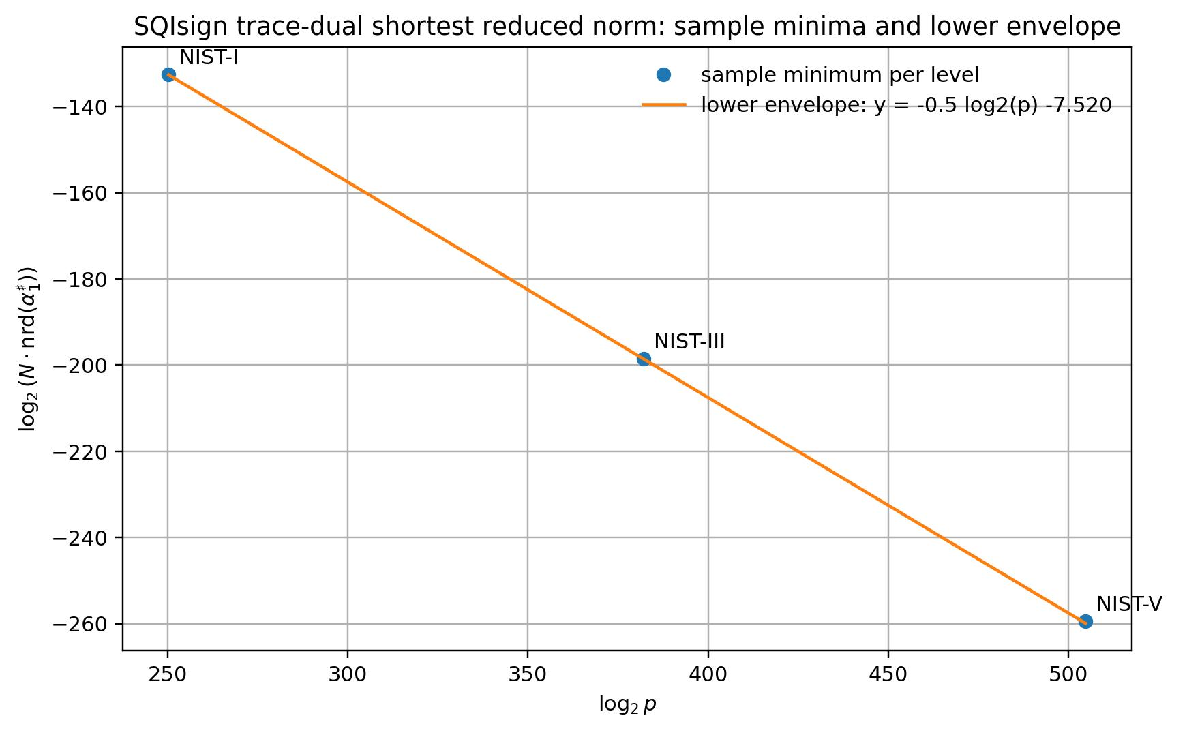
\includegraphics[width=\textwidth]{Figures/sqisign_trace_dual_transference_plot.pdf}
    \caption{Minimum over \(10{,}000\) samples of
    \(\log_2(D_{\mathrm{mix}}\operatorname{nrd}(\alpha_1^\#))\) for each NIST
    security level, where \(\alpha_1^\#\) is a shortest vector of the
    trace-dual lattice.}
    \label{fig:dual-norm}
\end{figure}


\section{Bound on IdealToIsogeny}
\label{sec:idealtoisogeny}

We now revisit the integer-size bound for
Algorithm~\ref{alg:IdealToIsogeny}.  The dominant arithmetic in this procedure
comes from the ideal operations used to prepare suitable short representatives.
In the previous analysis, this contribution was bounded using a coarse
worst-case estimate for ideal multiplication.  This was sufficient for the
correctness and asymptotic structure of the algorithm, since the remaining steps
were already bounded by the same dominant term.  However, after refining the
analysis of ideal multiplication, the same improvement can be propagated through
the subroutines used by \textsf{IdealToIsogeny}.

The first step is to update the bound for
Algorithm~\ref{alg:SuitableIdeals}.  This algorithm computes a reduced basis of
the input ideal and then searches for two short elements whose normalized norms
satisfy a Bezout relation modulo a power of two.  The search phase itself does
not introduce the largest integers: as in the previous analysis, the maximum
size occurs during the ideal multiplication required to compute the reduced
basis.  Therefore, replacing the old ideal multiplication estimate by
Lemma~\ref{lem:idealmult-bound} immediately yields a tighter bound for
\textsf{SuitableIdeals}.

\begin{algorithm}
\caption{SuitableIdeals$(I)$.}\label{alg:SuitableIdeals}
  \begin{algorithmic}[1]
    \Statex \textbf{Input:} A left $\mathcal{O}_0$-ideal $I$, a bound $d=\Theta(\sqrt{p})$.
    \Statex \textbf{Output:} $\beta_1,\beta_2\in I$ and $u,v\in\mathbb{N}^*$ and $f\le e$ such that $\gcd(u q_I(\beta_1),v q_I(\beta_2))=1$ and $u q_I(\beta_1)+v q_I(\beta_2)=2^f$.
    \State Compute a Minkowski reduced basis $(\alpha_1,\dots,\alpha_4)$ of $I$.
    \State Let $B_j\leftarrow \left\lfloor \frac{1}{4}\sqrt{\frac{d}{q_I(\alpha_j)}}\right\rfloor$ for $j\in[1;4]$.
    \State Sample $x_j\in [-B_j;B_j]^4$ for $j\in[1;4]$ and initialize $L\leftarrow [(x_1,\dots,x_4)]$.
    \For{$(y_1,\dots,y_4)\in [-B_1;B_1]\times\cdots\times[-B_4;B_4]$}
      \For{$(x_1,\dots,x_4)\in L$}
        \State $\beta_1\leftarrow \sum_{j=1}^4 x_j\alpha_j$ and $\beta_2\leftarrow \sum_{j=1}^4 y_j\alpha_j$.
        \State $d_1\leftarrow q_I(\beta_1),\ d_2\leftarrow q_I(\beta_2)$.
        \If{$d_1\equiv 1\pmod{2}$ and $d_2\equiv 1\pmod{2}$ and $\gcd(d_1,d_2)=1$}
          \State $u\leftarrow 2^{e} d_1^{-1}\bmod d_2$.
          \State $v\leftarrow \frac{2^{e}-u d_1}{d_2}$.
          \If{$v>0$}
            \State $e'\leftarrow \min(\nu_2(u),\nu_2(v))$, $u\leftarrow u/2^{e'}$, $v\leftarrow v/2^{e'}$, and $f\leftarrow e-e'$.
            \State \textbf{return} $\beta_1,\beta_2,u,v,f$.
          \Else
            \State Append $(y_1,\dots,y_4)$ to $L$.
          \EndIf
        \EndIf
      \EndFor
    \EndFor
  \end{algorithmic}
\end{algorithm}

The following lemma records the resulting refined bound.  Compared with the
previous accounting, the algorithm is unchanged; only the size analysis is
updated.  The improvement comes from using the sharper bound for the intermediate
ideal product appearing in the computation of the Minkowski reduced basis.

\begin{lemma}
During the execution of Algorithm~\ref{alg:SuitableIdeals}, the maximum size of integers is less than \[\frac{1024p^2}{\pi^4}\log{p} \cdot \nrd(I).\]
\end{lemma}

\begin{proof}
To compute a Minkowski reduced basis, one forms an ideal $\bar{J_t}I$ and its Gram matrix, then computes LLL-reduced basis~\cite{AAA+25}, where $J_t$ is the SQIsign parameter ideal.
By the proof of~\cite[Lemma~6]{KLKL25}, the maximum size of integers occurs by the ideal multiplication in Line~1.
Then, by Lemma~\ref{lem:idealmult-bound}, Lemma~\ref{lem:denombound}, and the fact that $\nrd(\bar{J_t}) < (\log{p})^2$, (See~\cite[Appendix~E]{KLKL25}.) we have the maximum size less than
\[
    \frac{1024p^2}{\pi^4}\log{p} \cdot \nrd(I).
\]
\end{proof}
We next propagate this refined estimate to
Algorithm~\ref{alg:IdealToIsogeny}.

\begin{algorithm}
\caption{IdealToIsogeny($I$)}\label{alg:IdealToIsogeny}
\begin{algorithmic}[1]
\Statex \textbf{Input:} A left $\mathcal{O}_0$-ideal $I$.
\Statex \textbf{Output:} The codomain $E_I$ of $\varphi_I$, $\varphi_I(P_0)$, and $\varphi_I(Q_0)$.
\State $u,v,e,s,t,\beta_1,\beta_2 \gets {\textsf{SuitableIdeals}}(I)$
\State $d_1 \gets \mathrm{nrd}(\beta_1)/\mathrm{nrd}(\overline{J_s}I)$
\State $d_2 \gets \mathrm{nrd}(\beta_2)/\mathrm{nrd}(\overline{J_t}I)$ \hfill {// $ud_1 + vd_2 = 2^e$, with $\gcd(ud_1,vd_2)=1$}
\State $E_u,\varphi_u(P_s), \varphi_u(Q_s) \gets {\textsf{FixedDegreeIsogeny}}(s,u)$ \hfill {// $\varphi_u: E_s \to E_u$ is an isogeny of degree $u$}
\State $E_v,\varphi_v(P_t), \varphi_v(Q_t) \gets {\textsf{FixedDegreeIsogeny}}(t,v)$ \hfill {// $\varphi_v: E_t \to E_v$ is an isogeny of degree $v$}
\State $[P,Q]^T \gets \left[\frac{1}{\mathrm{nrd}(I)\mathrm{nrd}(J_t)}\right] \mathbf{M}_{\beta_1} \mathbf{M}_{\beta_2} [\varphi_v(P_t), \varphi_v(Q_t)]^T$
\State $K_P \gets [2^{f-e}]([d_1]\varphi_u(P_s), P)$
\State $K_Q \gets [2^{f-e}]([d_1]\varphi_u(Q_s), Q)$
\State $E \times E', [(P,P'),(Q,Q')] \gets {\textsf{Isogeny22Chain}}(K_P, K_Q, [(\varphi_u(P_s), 0_{E_v}), (\varphi_u(Q_s), 0_{E_v})])$
\If{$e_{2f}(P,Q) = e_{2f}(P_s, Q_s)^{u^2 d_1}$} \hfill {// We identify the right curve $E_I$ by ensuring it is $d_1$-isogeneous to $E_0$}
    \State $E_I \gets E$, $P_I \gets P$, and $Q_I \gets Q$
\Else
    \State $E_I \gets E'$, $P_I \gets P'$, and $Q_I \gets Q'$
    \State $[P_I,Q_I]^T \gets \left[\frac{1}{ud_1}\right]\mathbf{M}_{\beta_1}[P_I,Q_I]^T$
\EndIf
\State \textbf{return} $E_I, (P_I, Q_I)$
\end{algorithmic}
\end{algorithm}

The improved bound for ideal multiplication, once inserted into \textsf{SuitableIdeals}, also gives the refined bound for the full \textsf{IdealToIsogeny} procedure.

\begin{lemma}
\label{lem:IdealToIsogeny-bound}
During the execution of Algorithm~\ref{alg:IdealToIsogeny}, the maximum size of integers is less than \[\frac{1024p^2}{\pi^4}\log{p} \cdot \nrd(I).\]
\end{lemma}

\begin{proof}
By following the same process of the proof of~\cite[Lemma~7]{KLKL25}, we have the same bound with Algorithm~\ref{alg:SuitableIdeals}.
\end{proof}


% \section{Implementation}


\begin{algorithm}
\caption{\textsf{LazySizeReduce}$(\kappa,\zeta,(b_1,\dots,b_d),G,\bar r,\bar\mu)$~\cite[Figure~5]{NS09}}
\label{alg:lazy-size-reduction}
\begin{algorithmic}[1]
  \Statex \textbf{Input:} An index $\kappa$, vectors
  $(b_{\zeta+1},\dots,b_\kappa)$, their Gram matrix $G$, floating-point numbers
  $\bar r_{i,j}$ and $\bar\mu_{i,j}$ for $\zeta+1\le j\le i<\kappa$,
  and fp-precision $\ell+1=53$.
  \Statex \textbf{Output:} Updated $b_\kappa$, $G$, and floating-point numbers
  $\bar r_{\kappa,j}$, $\bar\mu_{\kappa,j}$, and
  $\bar s^{(\kappa)}_j$ for $\zeta+1\le j\le \kappa$.

  \State $\bar\eta \gets \diamond(\diamond(0.55)+1/2)/2$.
  \State Compute the $\bar r_{\kappa,j}$'s, $\bar\mu_{\kappa,j}$'s, and
  $\bar s^{(\kappa)}_j$'s with steps 2--7 of the CFA with ``$i=\kappa$''
  for the vectors $b_{\zeta+1},\dots,b_\kappa$.
  \If{$\max_{\zeta+1\le j<\kappa} |\bar\mu_{\kappa,j}| \le \bar\eta$}
    \State \Return $(b_\kappa,G,\bar r_{\kappa,*},\bar\mu_{\kappa,*},\bar s^{(\kappa)}_*)$.
  \Else
    \For{$i=\kappa-1$ \textbf{down to} $\zeta+1$}
      \State $X_i \gets \lfloor \bar\mu_{\kappa,i}\rceil$.
      \For{$j=\zeta+1$ \textbf{to} $i-1$}
        \State $\bar\mu_{\kappa,j}\gets
        \diamond\!\left(\bar\mu_{\kappa,j}
        -\diamond(X_i\bar\mu_{i,j})\right)$.
      \EndFor
    \EndFor
    \State $b_\kappa \gets b_\kappa-\sum_{i=\zeta+1}^{\kappa-1}X_i b_i$,
    and update $G$ accordingly.
    \State \textbf{go to} line 2.
  \EndIf
\end{algorithmic}
\end{algorithm}

% \begin{algorithm}
% \caption{\textsf{ML2}$(b_1,\dots,b_d)$~\cite[Figure~9]{NS09}}
% \label{alg:ML2}
% \begin{algorithmic}[1]
%   \Statex \textbf{Input:} Nonzero vectors
%   $(b_1,\dots,b_d)\subset \mathbb{Z}^4$ generating a rank-$4$ lattice, and
%   fp-precision $\ell+1=53$.
%   \Statex \textbf{Output:} An $L^3$-reduced basis $(b'_1,\dots,b'_4)$.

%   \State Compute exactly $G=G(b_1,\dots,b_d)$.
%   \State $\bar\delta\gets \diamond(\diamond(3/4)+1)/2,\quad
%   \bar r_{1,1}\gets \diamond(\langle b_1,b_1\rangle),\quad
%   \kappa\gets 2,\quad \zeta\gets 0$.
%   \While{$\kappa\le d$}
%     \State $(b_\kappa,G,\bar r_{\kappa,*},\bar\mu_{\kappa,*},
%     \bar s^{(\kappa)}_*) \gets
%     \textsf{LazySizeReduce}(\kappa,\zeta,(b_1,\dots,b_d),G,\bar r,\bar\mu)$.
%     \State $\kappa'\gets \kappa$.
%     \While{$\kappa\ge \zeta+2$ \textbf{and}
%     $\diamond(\bar\delta\cdot \bar r_{\kappa-1,\kappa-1})
%     \ge \bar s^{(\kappa')}_{\kappa-1}$}
%       \State $\kappa\gets \kappa-1$.
%     \EndWhile
%     \For{$i=\zeta+1$ \textbf{to} $\kappa-1$}
%       \State $\bar\mu_{\kappa,i}\gets \bar\mu_{\kappa',i},\quad
%       \bar r_{\kappa,i}\gets \bar r_{\kappa',i}$.
%     \EndFor
%     \State $\bar r_{\kappa,\kappa}\gets \bar s^{(\kappa')}_\kappa$.
%     \State Insert $b_{\kappa'}$ right before $b_\kappa$ and update $G$ accordingly.
%     \If{$b_\kappa=0$}
%       \State $\zeta\gets \zeta+1$.
%     \EndIf
%     \State $\kappa\gets \max(\zeta+2,\kappa+1)$.
%   \EndWhile
%   \State \Return $(b_{\zeta+1},\dots,b_d)$.
% \end{algorithmic}
% \end{algorithm}

\begin{remark}
We restrict our setting to full-rank lattices in dimension $4$, hence
$k=\dim L=4$.
\cite[Figure~9, Theorem~10]{NS09} states its correctness with respect to the lattice rank $k=\dim L$ under the valid-pair condition
\[
  \frac14 < \delta < 1,
  \qquad
  \frac12 < \eta < \sqrt{\delta}.
\]
The choice $\eta=0.55$ is not merely arbitrary within the admissible interval; it is the exact value paired with $\delta=0.75$ in Section~3.4, Figure~7 of~\cite{NS09}.
Moreover, by~\cite[Figure~7]{NS09}, for $(\delta,\eta)=(0.75,0.55)$, double precision with $\ell=52$ is valid up to dimension $11$.
\end{remark}

% \begin{lemma}[Integer-size bound for \textsf{ML2}]
% \label{lem:ML2-bound}
% During the execution of Algorithm~\ref{alg:ML2}, the maximum size of integers is less than $\max_{1\le i\le d} || b_i ||^2$.
% \end{lemma}

\begin{proof}
The exact integer objects in Algorithm~\ref{alg:ML2} are the vectors $b_i$, or
equivalently the exact integral Gram matrix $G$. The quantities
$\bar r_{i,j}$, $\bar\mu_{i,j}$, $\bar s^{(\kappa)}_j$, and $\bar\delta$ are
fixed-precision floating-point numbers, and the indices $\kappa,\zeta$ do not
affect the integer-size bound.

We check the only steps that can affect exact integer data.

\smallskip
\noindent\textbf{(1) Initialization.}
In line~1, the algorithm computes
\[
  G_{i,j}=\langle b_i,b_j\rangle .
\]
By Cauchy--Schwarz,
\[
  |G_{i,j}|
  \le \|b_i\|\,\|b_j\|.
\]

\smallskip
\noindent\textbf{(2) Lazy size-reduction.}
Line~4 calls Algorithm~\ref{alg:lazy-size-reduction}. By
Lemma~\ref{lem:lazy-size-reduction-bound}, this subroutine does not increase
the size of any exact integer object beyond $B_{\rm in}$.

\smallskip
\noindent\textbf{(3) Insertion and remaining updates.}
Lines~5--12 only compare or copy floating-point quantities. Line~13 inserts
$b_{\kappa'}$ right before $b_\kappa$ and updates $G$ accordingly; this is just
a permutation of the current vectors and of the corresponding rows and columns
of $G$, so it creates no new integer magnitude. Lines~14--17 only test whether
$b_\kappa=0$ and update the indices $\zeta$ and $\kappa$.

Therefore every iteration of Algorithm~\ref{alg:ML2} preserves the invariant
that all exact integer objects are bounded by $B_{\rm in}$. Since the invariant
holds after initialization, it holds throughout the algorithm. Hence the exact
integer size in Algorithm~\ref{alg:ML2} is bounded by
\[
  \boxed{
  \max_{1\le i\le d}\|b_i\|^2
  } .
\]
\end{proof}

\begin{lemma}[Integer-size bound for \textsf{LazySizeReduce}]
\label{lem:lazy-size-reduction-bound}
Let
\[
  B_{\rm in}:=\max_{1\le i\le d}\|b_i\|^2
\]
be the initial input bound of Algorithm~\ref{alg:ML2}. Assume that before a
call to Algorithm~\ref{alg:lazy-size-reduction}, every exact integer object
currently stored by the algorithm, namely the vector representation or
equivalently the exact Gram-matrix representation, is bounded by $B_{\rm in}$.
Then the returned objects
\[
  b_\kappa,\qquad G,\qquad
  \bar r_{\kappa,*},\quad \bar\mu_{\kappa,*},\quad
  \bar s^{(\kappa)}_*
\]
do not increase the exact integer size beyond $B_{\rm in}$.
\end{lemma}

\begin{proof}
Algorithm~\ref{alg:lazy-size-reduction} manipulates two types of data: exact
integer data, namely $b_\kappa$ and the Gram matrix $G$, and fixed-precision
floating-point data, namely $\bar r$, $\bar\mu$, $\bar s$, and $\bar\eta$.
The floating-point quantities do not contribute to the integer-size bound.

Line~1 only assigns the floating-point value $\bar\eta$. Line~2 computes the
floating-point GSO quantities by the CFA procedure, using $G$ only as exact
input data and producing only rounded floating-point values. Hence lines~1--4
do not create any new exact integer magnitude.

The only nontrivial exact integer update occurs in lines~6--11, where
\[
  X_i\gets \lfloor \bar\mu_{\kappa,i}\rceil,
  \qquad
  b_\kappa\gets b_\kappa-\sum_{i=\zeta+1}^{\kappa-1}X_i b_i,
\]
and the exact Gram matrix $G$ is updated accordingly. This is precisely the
SizeReduce operation analyzed in~\cite{KLKL25}. By the SizeReduce integer-size
bound, this update does not increase the fixed exact-integer budget: after the
update, the reduced vector $b_\kappa$, or equivalently the updated row and
column of $G$, is again represented within the bound $B_{\rm in}$. All other
rows and columns of $G$ are unchanged.

Finally, line~12 only repeats the same procedure. Therefore, by induction over
the repetitions of Algorithm~\ref{alg:lazy-size-reduction}, the subroutine
returns without increasing the exact integer size beyond $B_{\rm in}$.
\end{proof}


% \section{Source codes for experiments}
\label{sec:code}

\subsection{Source code for Appendix~\ref{subsec:exp-basis}}
\label{subsec:code-basis}

\begin{lstlisting}[language=Python, caption={Experiment for the reduced norm of basis elements before ideal multiplication}, label={lst:sage_init}]

\end{lstlisting}

\subsection{Source code for Appendix~\ref{subsec:exp-dual}}
\label{subsec:code-dual}

\end{document}
